\documentclass[oneside, 12pt]{memoir}
\usepackage{verbatim}
\usepackage[labelsep=period, font=singlespacing, skip=12pt, format=hang, justification=RaggedRight, singlelinecheck=false]{caption}
\usepackage[T1]{fontenc}
\usepackage{times}
\usepackage{indentfirst}
\usepackage{thesis}
\usepackage{frontmattercontents}
\usepackage{listings}
\usepackage{graphicx}
\usepackage{hyperref}
\usepackage{layouts}
\usepackage{subfig}
\usepackage{algorithm2e}
\usepackage{amsmath}

\graphicspath{{./images/}}

\lstset{ %
xleftmargin=.2in,
xrightmargin=.1in,
language=Python,                	% choose the language of the code
basicstyle=\footnotesize,       % the size of the fonts that are used for the code
numbers=left,                   % where to put the line-numbers
numberstyle=\footnotesize,      % the size of the fonts that are used for the line-numbers
stepnumber=2,                   % the step between two line-numbers. If it's 1 each line 
                                % will be numbered                                                         
numbersep=5pt,                  % how far the line-numbers are from the code
showspaces=false,               % show spaces adding particular underscores
showstringspaces=false,         % underline spaces within strings
showtabs=false,                 % show tabs within strings adding particular underscores
frame=single,	                % adds a frame around the code
tabsize=2,	                	% sets default tabsize to 2 spaces
captionpos=b,                   % sets the caption-position to bottom
breaklines=true,                % sets automatic line breaking
breakatwhitespace=false,        % sets if automatic breaks should only happen at whitespace
title=\lstname,                 % show the filename of files included with \lstinputlisting;
                                % also try caption instead of title
escapeinside={\%*}{*)},         % if you want to add a comment within your code
morekeywords={*,...}            % if you want to add more keywords to the set
}


\checkandfixthelayout
\begin{document} 
	\setdoctype{Polemic}
	\masters 
	
	
\settitle{Modeling Mobile Web Characteristics for Energy Optimized Delivery}
\setauthor{Troy Johnson}

\setdefdate{September 2014}
\setgraddate{December, 2015}

\setchair{Dr. Patrick Seeling, Ph.D.}
\setmembers{Dr. Patrick Kinnicutt, Ph.D. \\ Dr. Michael Stinson, Ph.D.}


\newcommand{\titlepage}{{
\clearpage
\thispagestyle{empty}

\begin{SingleSpace}
\centering
\cmutitle \\
\vspace{1.42in} 
\cmuauthor \\
\vspace{1.42in}
A thesis submitted in partial fulfillment of\\
the requirements for the degree of\\
Master of Science \\
\vspace{2.333in}
Department of Computer Science \\
\vspace{2in}
Central Michigan University\\
Mount Pleasant, Michigan \\
September 2014\\
\end{SingleSpace}
\clearpage}}


\newcommand{\signaturepage}{{
\clearpage
\thispagestyle{plain}
{\centering
Accepted by the Faculty of the College of Graduate Studies,\\
Central Michigan University, in partial fulfillment of\\
the requirements for the master's degree\\}
\vspace{12pt}
{\noindent
Thesis Committee:\\}
\setlength{\tabcolsep}{0mm}
\begin{tabular}{{@{}l @{\hspace{10mm}}l}}
\rule{92mm}{.3pt}  &  Dr. Patrick Seeling \\
\rule{92mm}{.3pt}  &  Dr. Patrick Kinnicutt \\
\rule{92mm}{.3pt}  &  Dr. Michael Stinson \\
Date: \rule{81mm}{.3pt} & \\
\rule{92mm}{.3pt}  &  Dean \\ 
Date: \rule{81mm}{.3pt} & \parbox[tl]{2in}{\vspace*{-32pt} College of Graduate Studies} \\
\end{tabular}\\

{\noindent
Committee:\\
 
}
\clearpage}}

\newcommand{\acknowledgementspage}{{%
\clearpage
\thispagestyle{plain}

{\centering
ACKNOWLEDGMENTS \\}
Thanks to Dr. Seeling, Dr. Kinniccutt, Dr. Stinson, for ....This work was sponsored by an Early Career Grant from the Office of Research and Sponsored Programs at Central Michigan University. I also would like to wish thanks to A. Sampson and R. Kohvakka for their assistance in the development of the testbed measurement environment.
%\end{Spacing}
\clearpage}}


\newcommand{\abstractpage}{{
\clearpage
\thispagestyle{plain}

{\centering
ABSTRACT \\
\begin{SingleSpace}
\cmutitle \end{SingleSpace}
by Troy Johnson\\}

As mobile traffic and data consumption continue to rise, there is a growing need to investigate increased energy efficiency and optimizations to reduce the bandwidth when browsing the mobile web. To determine the reduction in energy consumption of mobile devices, there is also a need for a way to measure the energy consumption of mobile devices. By investigating the composition and characteristics of mobile web pages, statistical models can be derived for describing the characteristics of a typical mobile web page, such as the individual response sizes and expiration ages of responses that mobile browsers request for web pages. HTTP Archive will be a great source of data that may be utilized to derive models for describing the mobile web. Additionally, this pool of data is updated on a bimonthly basis, providing a constantly updated pool of data to update the developed models with and validate them. These models can then in turn be used to provide more accurate results when estimating the possible energy and bandwidth savings of optimizations by using these models for generating artificial web pages that will contain characteristics that closely resemble those characteristics often found on the actual mobile web.  Investigating the models and data further, they can be extended to create prediction models that will describe the growing mobile web for future years. With these models in place, they can be applied to projects for optimizing energy and bandwidth consumption on mobile devices, such as the possible energy and bandwidth savings that can result from cache forwarding between desktop computers and mobile devices. To measure the possible energy consumption savings from these projects, a low cost test bed for measuring the power consumption of mobile devices can be employed as a baseline. The measurement data ,experimentally determined, can then be used for follow-up performance analyses. 
\clearpage}}

	

\frontmatter
\setulmarginsandblock{0.75in}{1.25in}{*}
\titlepage
\clearpage
\pagebreak
\begin{Spacing}{2}
\acknowledgementspage
\clearpage
\pagebreak
\abstractpage
\clearpage
\pagebreak
\tableofcontents*
\clearpage
\pagebreak
\listoffigures
\clearpage
\pagebreak
\pagestyle{plain}
\checkandfixthelayout
\mainmatter
\counterwithout{figure}{chapter}
\addtocontents{toc}{\noindent CHAPTER \par}
\setulmarginsandblock{0.75in}{1.25in}{*} 

\chapter{INTRODUCTION}

\subsection{HTTP Archive}
HTTP Archive is an online repository of web performance information containing information on both desktop and mobile versions of websites. Information gather includes all the details about the responses each webpage makes such as the response sizes, expiration age, HTTP Archive gathers their data using a private instance of WebPageTest [CITATION????]. 

%Notes: Add more description in demonstration section
%Pull more specifics from the powepoint, also more
%description on the proxy overhead paper
\chapter{An Inexpensive Testbed for Mobile Device Power Measurement} 
\label{ch:testbed}


\section*{Introduction}
%addcontentsline add section to table of contents
\addcontentsline{toc}{section}{Introduction}

Over the last few decades, there has been an enormous increase in the ubiquity of mobile devices. With this increase, has also come the increase in demand for data-driven services and Cisco, Inc. predicts this demand to continue \cite{VNI14} into the foreseeable future. The battery consumption of mobile devices represents a limiting bottleneck and thus  power optimizations suggestions have been suggested \cite{Qian:2012:PTM:2187836.2187844} to reduce energy consumption on mobile devices. Software-based energy profilers do exist \cite{DAmato:2011:EAE:2419622.2419929}, however they are not always feasible for implementing in a straightforward manner or desirable due to rapid development cycles. To overcome these barriers, a real world test bed can be implemented  to perform measurements for the power consumptions on mobile devices to obtain a real life gauge for power estimations of optimizations. In this chapter, I will discuss the development and set up of a testbed for this purpose.

\addcontentsline{toc}{section}{Hardware Configuration}
\section*{Hardware Configuration}

The main component in this testbed is the mobile device.
This can be realized by using a smartphone and replacing the
battery with connectors to a power supply; alternatively one
of the common development board packages, such as
Pandaboard (see www.pandaboard.org) or Wandboard (see
www.wandboard.org) packages. Development boards and smartphones can be utilized together with the
Android operating system, which provides log output via USB
to the measurement control device, which can be a regular PC
or another development board with Android debugging
support. The mobile device is then networked with a wireless access point, which allows for wired and wireless evaluations.
The switchable power supply has an external serial or USB
port to communicate the current and power in small time
intervals to the control device. A BK Precision
1696 switchable power supply is utilized, as it offers fine granularity in power, current, and time intervals. While other equipment, such as an Arduino with custom circuits, were used in other measurement approaches, these power supplies are common lab equipment and offer overall robust features.

\addcontentsline{toc}{section}{Software Configuration}
\section*{Software Configuration}
The software components are comprised of several Python scripts that execute the Android Debugging Bridge (ADB) and capture the output either to a local file or allow sending of the output to a remote receiver, as illustrated in  Figure \ref{fig:testbed_setup}. These scripts allow for easy customization on the locally connected control device or at a remote location, e.g., filtering by specific events in the log. Similarly, a locally executing script captures the output from the power supply and is enabled to forward the data to a remote location as well.

\begin{figure}
\centering
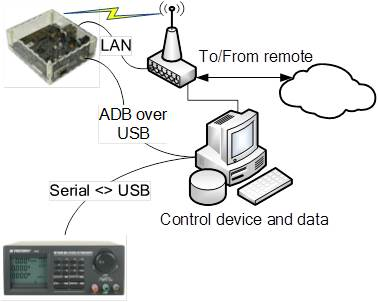
\includegraphics[scale=1,keepaspectratio,width=\columnwidth]{testbed_setup}
\caption{Illustration of measurement testbed.}
\label{fig:testbed_setup}
\end{figure}

\addcontentsline{toc}{section}{Demonstration Description}
\section*{Demonstration Description}
To demonstrate the usefulness of this testbed, two different aspects of the measurement setup were utilized using an example Android application that performs web requests (wired and wirelessly). This application makes requests to a local proxy server, either serially or in parallel, and the proxy server goes out and fetches what the phone requested.  The workflow for the application can be seen in figure \ref{fig:testapp_workflow}. Both, wired and wireless access scenarios were exhibited for accessing a remote web service and retrieving results in order to demonstrate the functionality of the testbed. With these demonstrations, real time visualizations of the data about power consumption were created and stored on log files on a remote computer where they can be readily parsed for automatic evaluation of application power consumption on the mobile device.

\begin{figure}
\centering
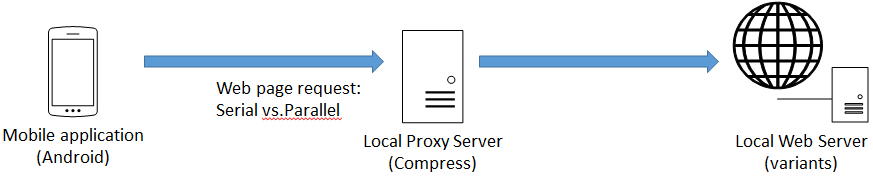
\includegraphics[scale=1,keepaspectratio,width=\columnwidth]{testapp_workflow}
\caption{Workflow of mobile application tested on testbed.}
\label{fig:testapp_workflow}
\end{figure}

%Notes:Talk about what exactly a proxy server is
\chapter{Power Consumption Overhead for Proxy Services on Mobile Device Platforms}

Current predictions by Cisco, Inc. show that the amount of data that users consume has increased significantly and will continue to increase into the foreseeable future \cite{VNI14}. Previous studies have shown that the network interfaces of mobile devices consume much of the limited battery life \cite{Carroll:2010:APC:1855840.1855861}. Thus, heavy research efforts have been poured into studying the possibilities of energy efficient mobile data delivery. Some research avenues have middleware that acts as an on-device proxy service to realize benefits or enable new interaction paradigms, such as display networks \cite{6174992} or mobile content sharing \cite{Seeling:2014:OES:2671189.2671194},\cite{6692468}. To determine whether or not local proxy servers result in a large overhead in terms of power consumption and time delays, the measurement framework testbed described in Chapter \ref{ch:testbed} can be implemented to determine what kind of overheads can be expected from utilizing local proxy servers.

\addcontentsline{toc}{section}{Methodology and Metrics}
\section*{Methodology and Metrics}

\addcontentsline{toc}{subsection}{Measurement Setup}
\subsection*{Measurement Setup}
To determine energy consumption, a set up similar to the one descibed in Chapter \ref{ch:testbed} is utlized. At the core of the setup, a Pandaboard ES mobile
software development platform is utilized, which features a Texas Instruments OMAP 4460 dual core ARM Cortex-A9 processor with
1 GB of DDR2 RAM, SMSC 10/100 Mbps Ethernet port, and
LS Research WLAN/Bluetooth wireless module, next to other
components. (Please refer to http://www.pandaboard.org for
more details. The open-source Android distribution
(version 4.1.2, ‘Jelly Bean’)  is used as the operating system software for the mobile device.
An illustration of the overall measurement setup can be seen in Figure \ref{fig:proxy_setup}. The
Pandaboard is powered by a BK Precision 1696 switchable
power supply, which features serial port access to read out
voltage and ampere values over time. The power
supply is connected to a Linux desktop computer serial port which timestamps
the values obtained over time to measure the power consumption
incurred by the Pandaboard. The Pandaboard is connected
through a 1 Gbps maximum speed Ethernet campus network,
which eliminates potential bottlenecks. For wireless measurements,
an externally connected WLAN antenna is utilized to
connect to the campus network through a dedicated WLAN access point, again eliminating potential bottlenecks for the
amounts of data considered throughout. It's also important to note
that a combination of input devices and an external monitor
were connected as well.
On the server side, a locally hosted virtual
machine next to Internet-routed web requests is utilized. The local server employs the Debian Linux distribution as its' operating system
with the Apache2 HTTP server and the popular Video Lan
Client (VLC) as the media streaming application. A pre-encoded
video sequence of the popular open-source movie Tears
of Steel (see http://www.tearsofsteel.org for more information) is streamed utilizing HTML5 video streaming. The video-only sequence
was transcoded offline into a resolution of 864 × 480 at 24
frames per second in the Theora video codec and encapsulated
using the OGG container format, both commonly utilized for
HTTP video streaming “on the web” and suitable for mobile
playout. The resulting video bit stream has a duration of 12
minutes, 14 seconds and an average bit rate of 1.42 Mbps.
The bit rate in turn falls well within range of the network
bandwidth capacity.


\addcontentsline{toc}{subsection}{Mobile SOCKSv5 Proxy Server}
\subsection*{Mobile SOCKSv5 Proxy Server}
Several implementations of the SOCKSv5 standard 
exist to date \cite{rfc1928}, which allow utilization of a remotely hosted
standard-conforming SOCKSv5 proxy server (typically from
a desktop computer through an organizational server). Mobile
implementations, however, are less frequent. One example
of an implementation for the Android operating system is
the anonymity generating Orbot application (see http://www.
torproject.us for more details), which routes traffic into the TOR network and contains “proxification” methods for applications as well (i.e., transparently forcing the usage of the proxy through, e.g., modifications of the iptables firewall). A basic Android service application was generated that is based on the jSOCKS proxy server implementation \cite{kouzoubov2011}, which is open source
(entirely written in JAVA) and does not require any
privileges, such as root level system access. As the service is executed within the Dalvik VM utilized on Android devices, it incurs a minimal computational overhead when compared to native applications. This approach, however, is commonplace to allow broadest application compatibility and encouraged for developers of the platform.

%Double check all equatons same as in paper
\addcontentsline{toc}{subsection}{Performance Metrics}
\subsection*{Performance Metrics}
In the following, we briefly outline the metrics used to evaluate the performance of either scheme. Initially, we capture the reported voltage level \textit{v(tl)} [V] and the current \textit{i(tl)} [A] as reported by the power supply and timestamped at time \textit{tl}
on the connected desktop computer. We similarly calculate
the instant power consumption as \textit{p(tl) = v(tl) * i(tl)} [W].
As the reported values are instantaneous snapshots in time
from \textit{l = 0} at \textit{t(l) = 0} (denoting the first measurement) to
\textit{l = L}, which happened at \textit{t(l) = T} (whereby \textit{T} denotes
the last measurement), we calculate the time passed between
consecutive measurement instances as $t(l) = t(l) - t_{l-1}$. To
determine the energy that was used in the \textit{l} - th measurement
period, we calculate $e(l) = t(l) * w(t_l)$ [J]. We denote the
energy that was used in a measurement period up to \textit{t(l)} as

\begin{equation}
o=\frac{\overline{E}_{Proxy} - \overline{E}_{Direct}}{\overline{E}_{Direct}},
\end{equation}
\newline

\begin{figure}
\centering
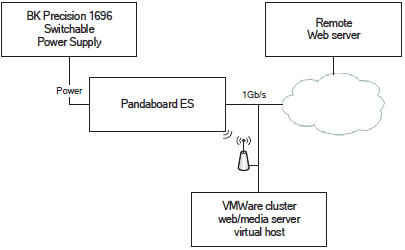
\includegraphics[scale=1,keepaspectratio]{proxy_setup}
\caption{Overview of the measurement setup}
\label{fig:proxy_setup}
\end{figure}

\addcontentsline{toc}{section}{Performance Evaluation For Web Requests}
\subsection*{Performance Evaluation For Web Request}
To perform a representative evaluation of frequent HTTP
web requests, web requests for Google’s home page were utilized.
The goal of this particular measurement scenario is to evaluate
the performance impact of frequent requests through the local
proxy server, which has to perform the additional connection
tasks each time a request is made. A direct
measurement application for Android was developed, which will request http://www.google.com without further resolving any
HTTP objects within. Individual requests are followed by a
sleep period of 2 seconds for both, direct requests and requests
through the mobile SOCKSv5 proxy service. As requests are
made without utilizing a browser, no caching is involved
client-side.

\addcontentsline{toc}{subsection}{Fixed Network}
\subsection*{Fixed Network}
In the fixed network scenario, the Pandaboard is connected
through wired Ethernet to the campus network while performing
the web requests. The requests typically coincide
with high power consumption levels, as illustrated in Figure \ref{fig:proxy_energy_cons_socks}
for an exemplary 100 web requests with both configurations.
We observe that both approaches exhibit an initial “spike”
behavior and an otherwise low level (with some general noise
due to overall device activities). There is no immediately
visible trend for the momentary power consumptions, as in
both approaches, there are several bursty periods of slightly
elevated consumptions on top of the actual web requests.
Next, we evaluate the total (compounded) energy consumption
that is observed when performing these requests for a
certain period of time. We illustrate 100 subsequent requests
directly and through the mobile proxy server in Figure \ref{fig:proxy_comp_energy_cons}.
Initially, it is observed that despite the short-term fluctuations,
there is a linear increase in the energy consumed
while using either approach. More significantly, there is no
immediately noticeable significant difference between the
approaches, which is indicated by the almost indistinguishable
values in the plot. Lastly, comparing the overhead between
the approaches numerically in Table \ref{tab:requests_summary}, where the
300 highest levels of energy consumption measured for periods
of placing 300 requests were analyzed. It's also notable that the direct approach
results in a higher average level of energy consumption (albeit
with a larger variability), whereas the proxy-based approach
yields a lower average and variability of energy usage values
determined. Overall, this results in an overhead of o =
−0.0563, which presents an initially counter-intuitive result.
(Differently worded, by utilizing the mobile proxy server
consuming additional CPU cycles, potential energy savings
of 5.6\% could be realized without requiring any additional
modifications.) Taking into account that partially significant
variability exists due to some outliers in the total duration
(as some measurement points can exhibit significant delays or
coincide with other unrelated system activities), both approaches are very similar.

\begin{figure}
\centering
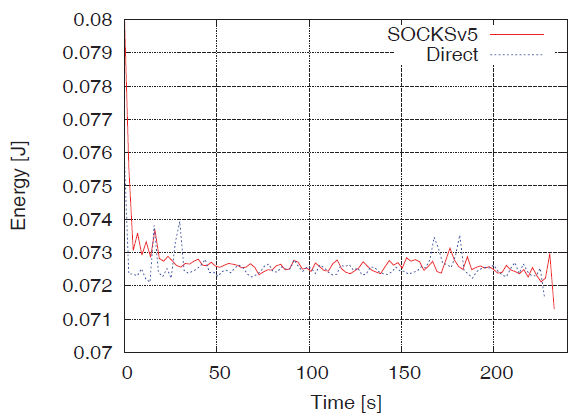
\includegraphics[scale=1,keepaspectratio]{proxy_energy_cons_socks}
\caption{Energy consumption while performing 100 web requests directly or through a mobile SOCKSv5 service, smoothed over time.}
\label{fig:proxy_energy_cons_socks}
\end{figure}

\begin{figure}
\centering
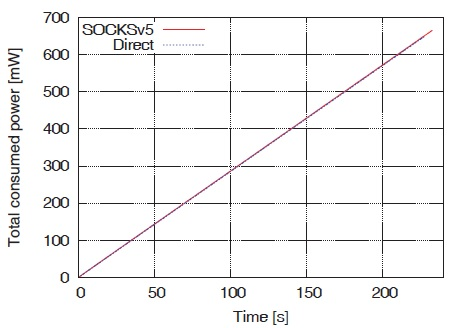
\includegraphics[scale=1,keepaspectratio]{proxy_comp_energy_cons}
\caption{Compounded energy consumption for performing 100 web requests directly or through a mobile SOCKSv5 service.}
\label{fig:proxy_comp_energy_cons}
\end{figure}

\begin{table}[h]
\begin{tabular}{|c|c|c|c|c|}
\hline
 Interface & Approach  & Average[J]  & Standard Deviation [J] & Confidence Interval (99 \%)  \\ \hline
 LAN & Direct & 0.0912 & 0.0139 & 0.0021 \\ \hline
 LAN & Proxy & 0.0860 & 0.0062 & 0.0009 \\ \hline
 WLAN & Direct & 0.0900 & 0.0125 & 0.0019 \\ \hline
 WLAN & Proxy & 0.0902 & 0.0089 & 0.0013 \\ \hline
\end{tabular}
\caption{Summary values for 300 direct and proxy-routed web requests over traditional ethernet and wireless LAN networks.}
\label{tab:requests_summary}
\end{table}

\addcontentsline{toc}{subsection}{Wireless Network}
\subsection*{Wireless Network}
Shifting the evaluation to HTTP requests made over the
wireless network interface, we present our results in Table \ref{tab:requests_summary}.
(We note that a graphical evaluation would yield results similar
to those presented in Figures \ref{fig:proxy_energy_cons_socks} and \ref{fig:proxy_comp_energy_cons}.) We initially note that
both approaches are very close with respect to their measured
average energy consumption, resulting standard deviations,
and narrow confidence intervals. \newline
Comparing these results with those obtained for the Ethernet
scenario, which outlines the base case without active wireless
communications overheads, we do not note a significant difference
in the average energy usage for the individual web
requests.

\addcontentsline{toc}{section}{Impact of Web Request Variations}
\subsection*{Impact of Web Request Variations}
Motivated by the closeness of requests, the next step is to more
closely evaluate the impact of the web request size over a
wireless LAN on the overall power consumption. To limit
the impact that external networks can have (such as different
delays), the direct performance comparison is performed within
the on-campus VM environment illustrated in Figure \ref{fig:proxy_setup}. A
dedicated virtual machine uses the Apache2 web server and
hosts a Python script that generates a requested number of
bytes, additionally eliminating potential caching impacts. 100 repeated measurements are performed for each different web request size and significant outliers are deleted.

\addcontentsline{toc}{subsection}{Power Consumption}
\subsection*{Power Consumption}

\begin{figure}
\centering
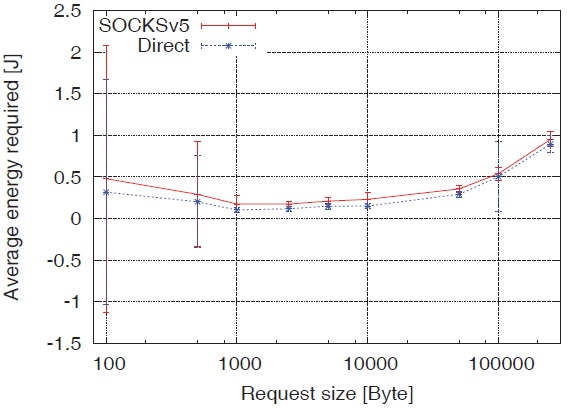
\includegraphics[scale=1,keepaspectratio]{energy_cons_direct_vs_socks}
\caption{Average energy consumption and standard deviation for requesting different amounts of data from a local server using a direct or mobile SOCKSv5 proxy server.}
\label{fig:energy_cons_direct_vs_socks}
\end{figure}

\begin{figure}
\centering
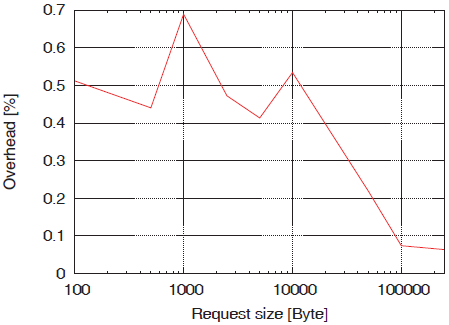
\includegraphics[scale=1,keepaspectratio]{energy_cons_overhead}
\caption{Average energy consumption overhead for requesting different
amounts of data from a local server}
\label{fig:energy_cons_overhead}
\end{figure}

The average energy used per different request size is illustrated in in Figure \ref*{fig:energy_cons_direct_vs_socks}. It's observed that the mobile SOCKSv5 proxy approach always incurs a penalty
over the direct connection, which is readily explained by the
additional local processing overhead on the device. Furthermore,
it can be noted that both depicted connection methods follow
a “slump”-like behavior. Taking the overall variability of
measurements into account, until the amount of requested data
approaches the single packet payload region, the lowest energy
usage is recorded. This initial behavior can be explained
by the overhead to establish the initial server connection,
which is dominant for the small request size regions. With
a further increase of the payload to very large sizes, the
number of required transmissions drastically increases, which
now accounts for the majority of the energy consumption
(rather than the initial connection setup). This increase in the
number of packets is now causing longer periods of energy expensive
network activities, causing the rise in energy consumption
illustrated. The overall absolute difference between
the employment of a mobile proxy and direct connection,
however, remains fairly constant, which indicates that the
processing overhead for local packet processing prior delivery
to an application is rather negligible.
Next, the overhead incurred by the mobile
proxy server (as in Equation 1) in Figure \ref{fig:energy_cons_overhead}.Initially,
an overall “hump”-like behavior is observable which decreases as
the request sizes increase. Part of this behavior is explained
by the rather large variability (which isn't illustrated
here for clarity) in the regions of smaller request sizes. The overall diminishing overhead is explainable by the increase in the web request sizes with the actual overhead in the
processing and local loop-back data connections for the proxy
service. As the proxy service requires an initial connection
setup before performing the pass-through connection from the
remote server, additional time and processing resources are
required before the connection can be fully passed through
the proxy. Both resources incur processing and delay penalties
which in turn have negative power consumption impacts.
Larger request sizes result in increased numbers of packets
to transmit, which “smoothes” the fixed setup overhead over
more packets, which results in the decreasing overhead. At
250 kB of requested data, an observable reduction occurs to just below
six percent. Overall, that based on these measurements, it's observed that the implementation of a mobile proxy server directly on a
mobile device does not result in considerable additional power
demands for larger-sized web requests, which are common
today.

\addcontentsline{toc}{section}{Delay Difference}
\subsection*{Delay Difference}
With most interactive settings, the overhead in terms of
additional delays can have a negative impact on user utility
or perceived quality of service. In networked mobile settings,
increased delays additionally have a negative battery impact
through the direct correlation between the two.
The average delay differences between the proxy and the direct
connections for different request sizes is illustrated in Figure \ref{fig:time_difference_requests}. Initially,
there is a fairly steady level of added average delays to the
mobile proxy service in the region of 25 ms with higher levels of standard deviation occurring where the larger amounts
of data requested; an overall maximum of about 37 ms can
be noted for requesting 250 kB of data. The variability for
the delays is a combination of the script producing the larger
chunks of data with now slightly increased variability, as well
as the increased number of packets sent for each approach
incurring an additional network delay variation.
Overall, it can be concluded that the observed low level of additional
delay represents the fairly constant overhead of setting
up the proxy service on the mobile device and processing the
initial connection requests.

\begin{figure}
\centering
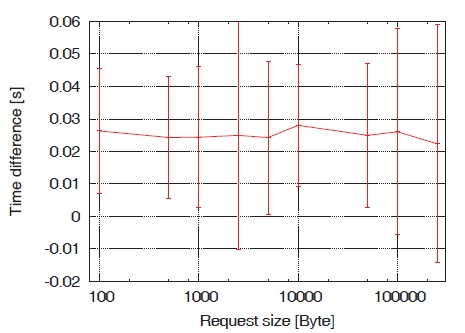
\includegraphics[scale=1,keepaspectratio]{time_difference_requests}
\caption{Average time difference and standard deviation between the direct and the proxy approach for requesting different amounts of data from a local server.}
\label{fig:time_difference_requests}
\end{figure}

\addcontentsline{toc}{section}{Media Streaming}
\subsection*{Media Streaming}
The next step is to evaluate the impact of a long duration
connection through the mobile SOCKSv5 server, in contrast
to the previous evaluation of frequent connection requests.
Here, a continuous data stream needs to be forwarded to a
local application, with the initial setup overhead becoming
negligible. The playback of the web video on the Pandaboard
is performed using the Firefox for Android web browser. For
measurements of the incurred proxy overhead, the browser
is reconfigured to utilize the local SOCKSv5 proxy service,
similar to the previous web request scenarios. The HTML5
video is in turn displayed on the browser for the entire
duration.

\begin{figure}
\centering
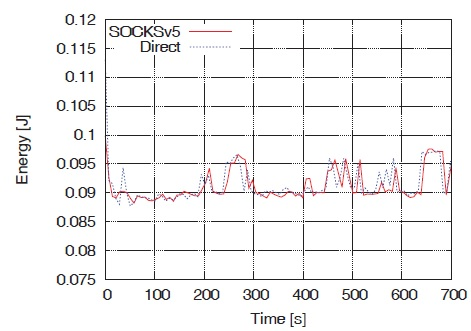
\includegraphics[scale=1,keepaspectratio]{video_streaming_cons_socks}
\caption{Energy consumption while performing the video streaming of the
Tears of Steel open-source video sequence directly and through a mobile
SOCKSv5 proxy server, smoothed over time.}
\label{fig:video_streaming_cons_socks}
\end{figure}

\addcontentsline{toc}{section}{Fixed Network}
\subsection*{Fixed Network}
The sampled power consumption for video
streaming over a wired Ethernet network is illustrated in Figure \ref{fig:video_streaming_cons_socks}. Observing the graph, we can
see that most of the measured power consumption values
fall into a range between 3.25 W and 3.75 W for both
approaches. Both approaches additionally exhibit overall periods
of heightened power consumption, e.g., from about
250s to about 290s. This time frame coincides with a fast
camera movement following an actor (very high level of
background content change, motion) and represents a more
challenging video decoding task, in turn leading to higher
power consumption. Comparatively, however, it's also observable that no
significant differences exist between the two approaches. The aggregated
energy consumption resulting from media streaming
results in a linear behavior, which additionally is almost
indistinguishable between the two approaches as observed
for the prior web requests scenario. As indicated by the
comparable energy consumption over time in Figure \ref{fig:video_streaming_cons_socks}, the
additional video decoding power requirements let the overall
power consumption differences remain minor. We in turn omit
a visual representation that closely resembles Figure \ref{fig:proxy_comp_energy_cons} due
to space constraints. The aggregated performance
values for this scenario in Table \ref{tab:agg_perf_results}. NEED TO CHANGE THIS TO TABLE FORMAT IN LATEX INSTEAD OF PICTURE) Looking at the table, I note that the average
energy used is very similar for either approach, with slightly
elevated values for the direct approach. Taking the standard
deviation and the very narrow 99\% confidence intervals into
account, we note that the proxy-based streaming incurs no
significant penalties. Comparing this streaming example to the
individual web requests, I note that overall, the proxy-based
approach now is at the same overall level that I observed
for the direct case.

\begin{figure}
\centering
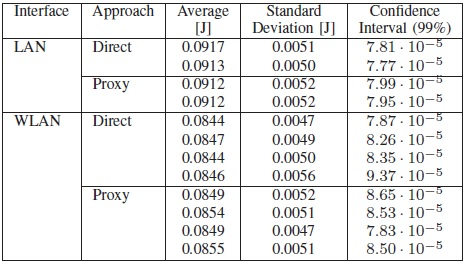
\includegraphics[scale=1,keepaspectratio]{agg_perf_results}
\caption{Summary values for HTML5 video streaming of the open-source Tears of Steel movie (video-only) over an ethernet and a wireless network.}
\label{tab:agg_perf_results}
\end{figure}

\addcontentsline{toc}{section}{Wireless Network}
\subsection*{Wireless Network}
As in the previous web request scenario, I additionally
investigate the alternative approach whereby the video streaming
is now utilizing a local wireless network.  The
measurement results in Table \ref{tab:agg_perf_results} for equal numbers of measurement
points. (Also note that for means of better comparison,
the number of measurement points are limited to be equal.) I
note that the overall averages are fairly close and furthermore
characterized by relatively narrow confidence intervals. The
resulting overhead, when comparing the averages of the direct
and proxy-based video streaming is 0.0081, or less than one
percent. Comparing the overall WLAN levels to the wired
measurements, I note a decrease in the overall power consumption.
This behavior is explained with the full availability of
all network interfaces, whereby the employed operating system
seems unable to properly put all different interfaces into a nopower
state.
Overall, I conclude that the introduction of the mobile
proxy server has only limited negative impacts on the power
consumption of about one percent when streaming multimedia
due to the significantly higher impact of the decoding processes
on the energy consumption and the negligible packet
processing overheads.



\addcontentsline{toc}{section}{Conclusions and Future Work}
\subsection*{Conclusions and Future Work}
I approximated the energy consumption overhead of
mobile optimization frameworks through a mobile SOCKSv5
proxy server as a low-end baseline. The selected implementation
is based on JAVA and performs all network traffic
forwarding on the application layer within the Dalvik VM for
Android devices. I found that the overall usage of a proxy
service on the mobile device in a web request scenario does
not incur any significant power consumption penalties. For
HTML5 video streaming (continuous packet processing), I
note an overhead of about one percent. I determined that any
existing overhead is relatively constant and explained through
the initial communication setup overheads, rather than ondevice
processing overheads, which were found to be approximately one
percent. A basic optimization framework would in turn only
need to overcome this very low overhead to enable energy
savings potentials.In future research avenues, I plan to investigate further energy savings potentials based on mobile device proxying,
in combination with caching and application layer content
awareness in tandem with a remote server.
\chapter{Web Cache Object Forwarding From Desktop to Mobile for Energy Consumption Optimizations}

\section*{Introduction}
\addcontentsline{toc}{section}{Introduction}

With the beginning of the 21st century, networking support for wirelessly connected mobile user devices has fueled a continuous increase in the demand for mobile data.
Web requests now originate in a majority from wirelessly connected user devices -- a trend that Cisco, Inc. predicts to continue in the foreseeable future~\cite{VNI14}.
Simultaneously, the overall user behavior and demand for more rich media inclusion into web pages has increased the overall amount of data that is required to be transmitted per page, see, e.g., \cite{IhPa11,BuMaSe13}.
Caching on the client side has been effectively used in the past and was, together with increased numbers of parallel object downloads, able to decrease wait times for desktop clients as reported in \cite{IhPa11}.
A first view of mobile web page characteristics (which were found to exhibit lower complexity than regular desktop browser versions) and non-landing pages (which were found to be less complex than landing pages) was evaluated by the authors of~\cite{BuMaSe13}.
Moreover, a significant body of research has emerged that focuses on content delivery optimizations to mobile devices.

Typically, these optimization approaches are targeting on-device optimizations or off--device cloud--based improvements.
For mobile applications, for example, significant energy savings were found to be attainable when grouping application requests so as to avoid prolonged cellular network interface activity, see, e.g., \cite{BaBaVe09,QiWaGaHuGe12}.
Other approaches optimize the delivery to mobile devices through proxies and cloud-based data anticipation and traffic shaping, see, e.g., \cite{XiHuSaYl11}.

For web data, typically caching is used to limit the amount of data that has to be transfered to requesting clients.
In prior works focusing on mobile web page delivery optimizations, such as \cite{SaIs02}, energy optimization has been a key element, due to the limiting restrictions for mobile clients.
One particular area for optimization is the pre--fetching of web page objects combined with caching (which allows to download data before usage), such as presented in~\cite{ShKuDaWa05} with about 10 \% energy savings.
More recently, these approaches were combined with user connectivity predictions, see, e.g., \cite{ThChWo13}.

\begin{figure}
\centering
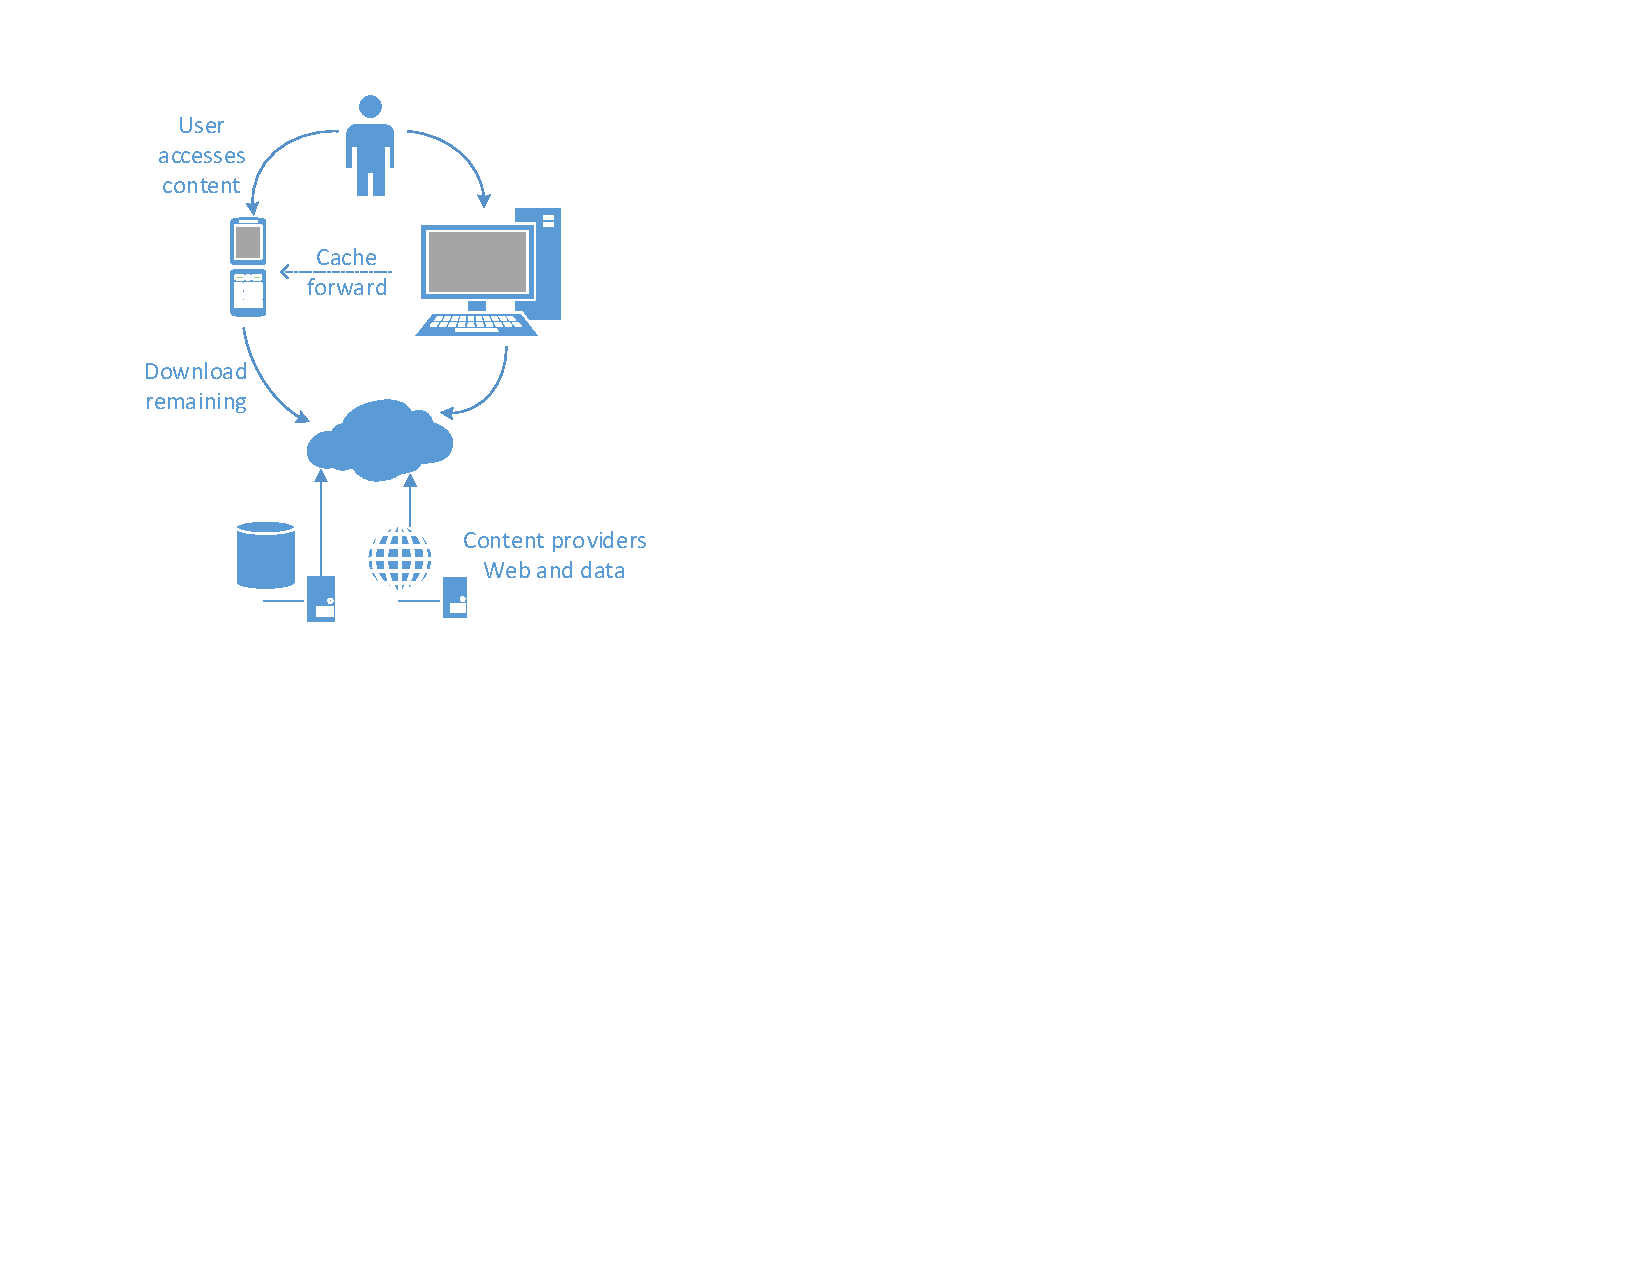
\includegraphics[scale=1,keepaspectratio]{cache_forwarding_setup}
	\caption{Screenshot of rendered web page from WebPageSpeedTest.org. As illustrated, the main textual and pictorial content items are flanked by background and interactive advertisements.}
\label{fig:cache_forwarding_setup}
\end{figure}

We propose to utilize a basic cache forwarding method that can be utilized by users to synchronize from, e.g., a desktop computer, to their mobile device, e.g., a smartphone.
We illustrate this approach in Figure~\ref{fig:cache_forwarding_setup}, which contains the desktop and a mobile device. 
As most devices are charged over night, or are at least stationary within local area network ranges, we propose to utilize this general idle period to allow direct forwarding of cached objects.
We presume that browser clients will have a shared information source in the cloud that allows the identification of visited web pages, an approach most browser clients take to date.
In turn, clients are enabled to identify web page objects that are identical between the different device display modalities, i.e., identical web objects delivered when requesting a desktop/mobile versions of a web page.
The thus transmitted objects, in turn, reside locally within the mobile device cache and do not require an energy--expensive mobile download through cellular interfaces. 
We note that the reverse of this approach is possible as well.
To support our approach, we gather data through the publicly accessible \url{WebpageSpeedTest.org} website as well as the \url{httparchive.org} archive of a large dataset of performance evaluations for popular web pages; we refer the interested reader to~\cite{Me13} for a more detailed discussion.

\section*{Individual Example}
\addcontentsline{toc}{section}{Introduction}
\label{s:example}
In this section, we outline an individual example for the German news web page ``Der Spiegel,'' accessible at \url{http://www.spiegel.de}.
This web page serves as an example for a rich media and advertising material containing web presence that is frequently updated.
On February 12, 2014, we performed a speed test online using ($i$) Internet Explorer 9 as the browser instance for a desktop client, ($ii$) Chrome as the mobile browser on a Google Nexus 5 instance, and ($iii$) Safari for an iPhone 4 instance provided by \url{WebpageSpeedTest.org} (both mobile clients were traffic shaped to 3G connection emulations).
An example screenshot of the web page as rendered is provided in Figure~\ref{fig:screens}.
\begin{figure}
\centering
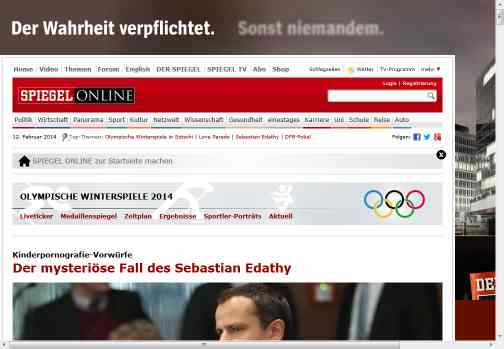
\includegraphics[scale=1,keepaspectratio,width=\columnwidth]{1screen}
	\caption{Screenshot of rendered web page from WebPageSpeedTest.org. As illustrated, the main textual and pictorial content items are flanked by background and interactive advertisements.}
\label{fig:screens}
\end{figure}

As illustrated, the web page exhibits a significant amount of objects that are required for advertisements, visual items (images, layout), and scripting.

We evaluate the reported data as follows. 
For each display modality and browser client, we gather the individual web objects requested and the response sizes and headers for caching information (for HTTP response codes 200 only, as we are not interested in redirects).
We denote the number of all objects returned for a request modality (i.e., Internet Explorer for the desktop client example and iPhone or Nexus 5 for mobile counterparts) as $N$, their average size as $\overline{X}$, the standard deviation of their sizes as ${\sigma}_{X}$, and the Coefficient of Variation (CoV) of the returned object sizes as $\mathrm{CoV}_{X}$. 
As in the HTTP specification, the \emph{max--age} directive overrides others, so we initially consider that directive for the cache longevity of the individual objects. 
If no explicit information is found, we consider the response header's \emph{expires} information, which provides a secondary cache lifetime. 
If both are not found, or if the \emph{expires} date is in the past or right at the request time, we set the cache lifetime to zero. 
Similar to the notation for the object sizes, we denote the expiration time characteristics as $\overline{T}$, $\sigma_{T}$, and $\mathrm{CoV}_{T}$, respectively.

\subsection*{Data Description}
\addcontentsline{toc}{subsection}{Data Description}

We provide an initial high-level overview of the web page characteristics for \url{http://www.spiegel.de} as requested by the different clients in Table~\ref{tab:spiegel}.
\begin{table}
\centering
\caption{High-level overview of different client web page statistics for http://www.spiegel.de}
\label{tab:spiegel}
\begin{tabular}{|l|r|r|r|}
	\hline
	Statistic          & IE Deskt. &    iPhone &   Nexus 5 \\ \hline
	$N$                &       154 &       132 &       145 \\ \hline\hline
	$\overline{X}$     &  10402.77 &   8846.39 &  10201.63 \\ \hline
	$\sigma$           &  19103.19 &  13438.05 &  25684.58 \\ \hline
	$\mathrm{CoV}_{X}$ &      1.84 &      1.52 &      2.52 \\ \hline\hline
	$\overline{T}$     & 106285.14 & 114780.69 & 114818.28 \\ \hline
	$\sigma_{T}$       & 125080.27 & 125576.65 & 126090.90 \\ \hline
	$\mathrm{CoV}_{T}$ &      1.18 &      1.09 &      1.10 \\ \hline
\end{tabular}
\end{table}

We initially observe that the desktop version (with Internet Explorer 9 as requesting browser client) exhibits the highest number of objects, followed by the mobile Chrome/Android and Safari mobile/iOS versions.
Interestingly, there is only a minor difference in the number of objects between these versions.
Next, we observe that the trend for the average number of bytes is aligned with the number of elements. 
In total, the mobile Chrome version is almost on par with the desktop one (at 92~\% of total data); only the Safari mobile version seems optimized (at 72~\% of total data).
The standard deviation and Coefficient of Variation (CoV) amongst individual element sizes are highest for the mobile Chrome version, indicating more significant size differences than for the safari version (which is one unit lower), while the desktop version falls into the middle.

Next, we evaluate the elements' caching properties on a high level as presented in Table~\ref{tab:spiegel} as well. 
Overall, we note that the highest average caching time is observed for the mobile Chrome access with the Nexus 5 device, trailed immediately by the iOS access and (with distance) by the desktop browser.
We note that the overall variability in terms of expiration times amongst elements is fairly low and comparable, as indicated by CoV values around 1.1.

\subsection*{Evaluation of Local Cache Forwarding}
\addcontentsline{toc}{subsection}{Evaluation of Local Cache Forwarding}
We now shift the view to the possibility for identical objects to be re--utilized locally to avoid additional download penalties in time and energy consumption.
Simultaneous with a web page request, a local broadcast could ``ask'' for the cached elements for a website to be delivered locally from participating clients. 
Alternatively, cellular provisioning methods, such as in LTE--A, could initiate the device--to--device local exchange as well.
Once the request is received, the local coordination can take place, which inherently results in the forwarding of elements that are the same across browser instances and which have a future cache lifetime expiration.

We filter out elements that are not similar amongst the different requesting devices, which results in 82 objects with the same URL and size combination. 
In other words, just above half of the objects constituting the web page under consideration are identical between different clients.

While we note an identical cache lifetime for most of these objects, a slight increase is notable from the Desktop over Safari to Chrome clients.  
Next, we remove items that exhibit a cache lifetime of zero for any of the three requesting clients, resulting in 59 objects.
These remaining objects display a reduced average cache lifetime for the mobile browsers, whereby mobile Chrome exhibits the shortest.
In turn, we choose the iOS Safari mobile as our exemplary base for calculations. 
We utilize the approximations for energy consumptions presented in~\cite{PeFiWi11} to determine the amount of energy required if local data forwarding can be performed using either Bluetooth or WLAN technologies. 
We illustrate the energy consumption as function of time in Figure~\ref{fig:ios_time_energy}.
\begin{figure}
\centering
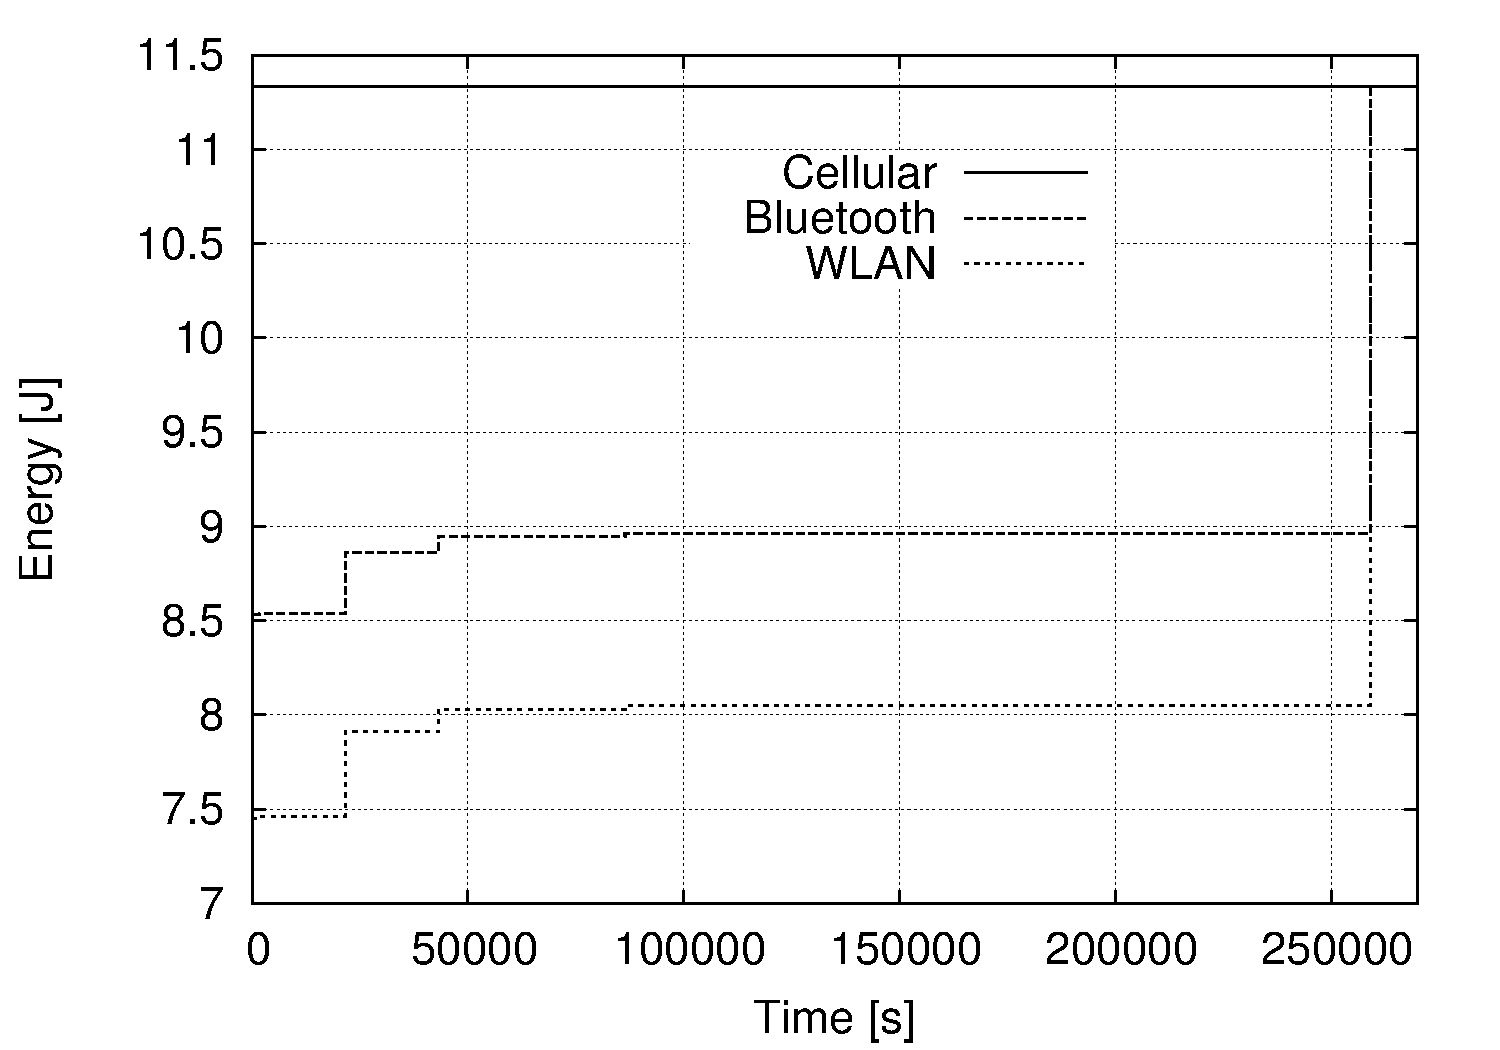
\includegraphics[scale=1,keepaspectratio,width=\textwidth]{energy_ios_time}
		\caption{Energy required to download web page data via cellular connection or through combination with partial local exchange with Bluetooth/WLAN.}
\label{fig:ios_time_energy}
\end{figure}

The complete download energy for exclusive use of cellular is the upper limit on energy spent downloading the data associated with the web page. 
The Bluetooth and WLAN data exchanges with other local clients both follow the same underlying trend with increasing energy required to transmit all data as time progresses from the last access point in time (due to cache expirations).

We illustrate the relative amount of data/items within the cache in addition to the attainable savings in Figure~\ref{fig:rel_ios_time} as a function of delayed access time. 
\begin{figure}
\centering
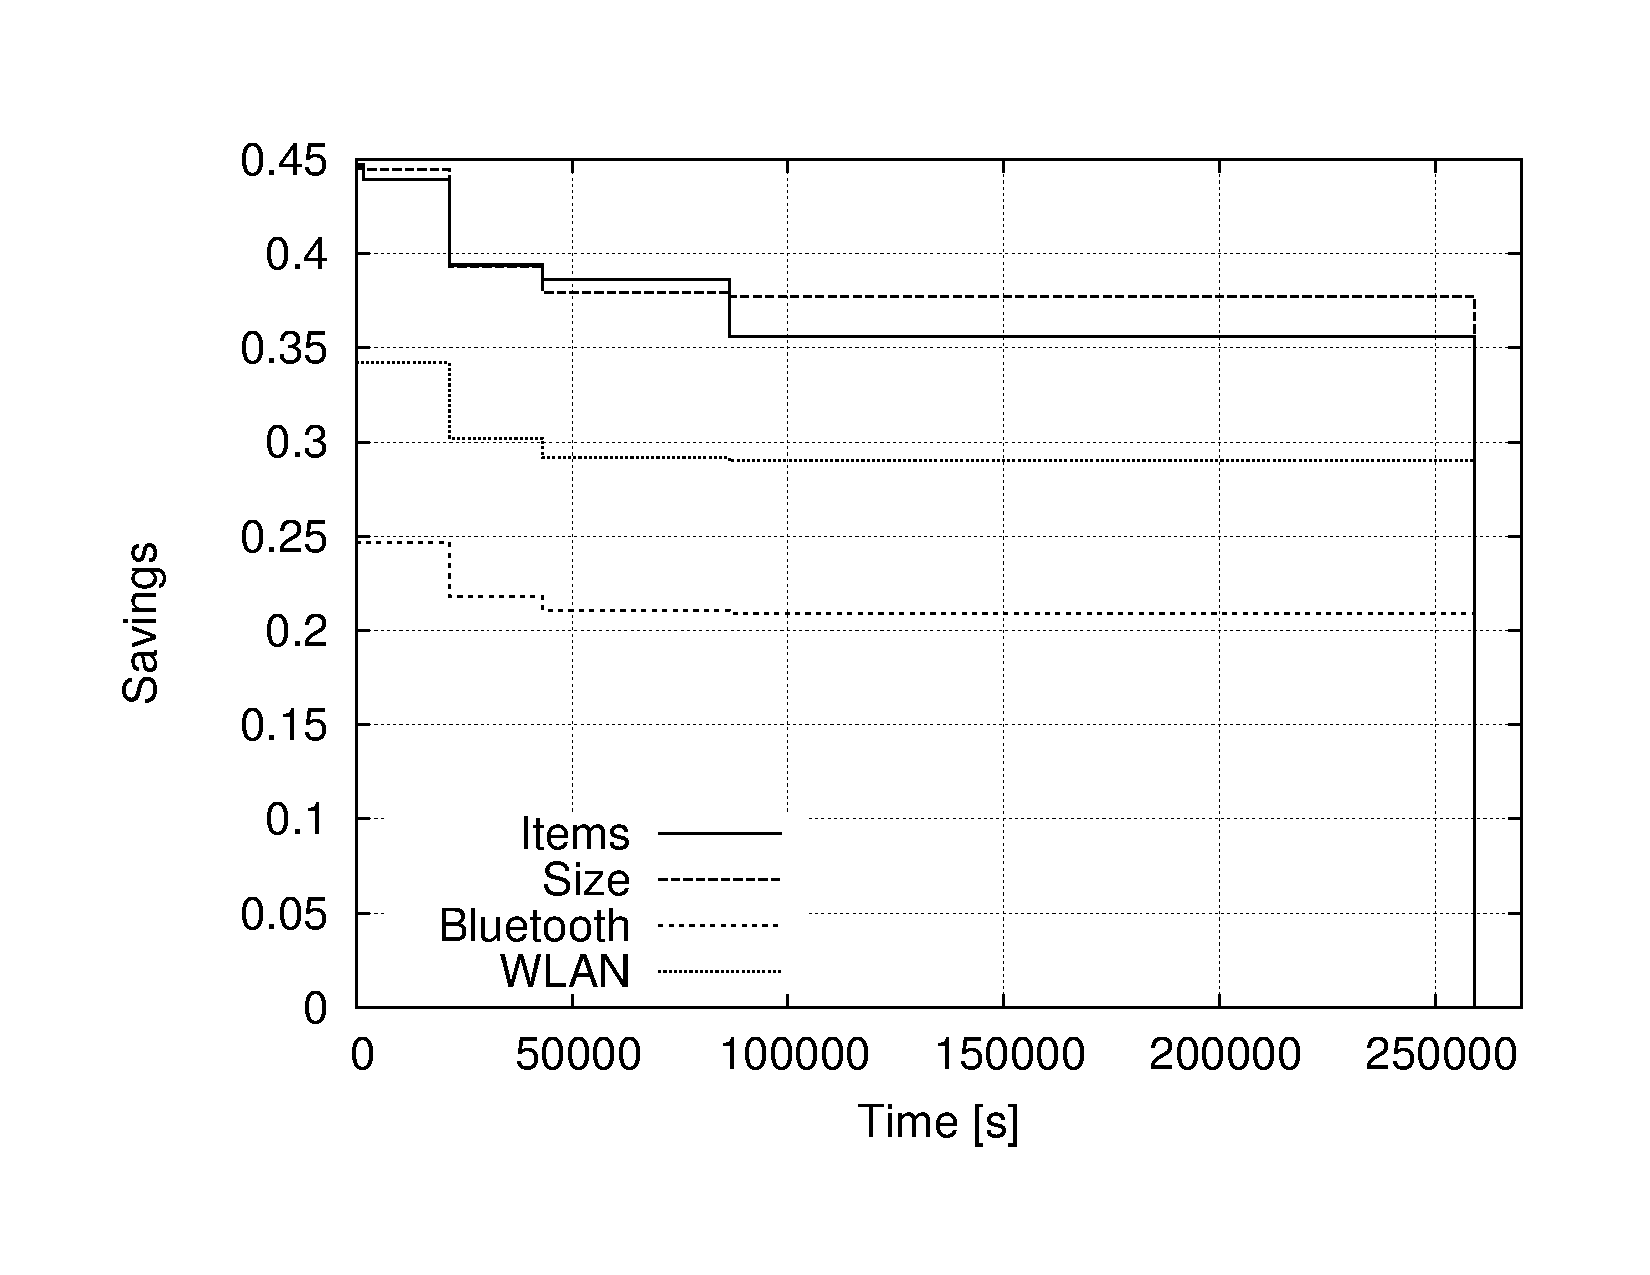
\includegraphics[scale=1,keepaspectratio,width=\columnwidth]{rel_ios_time}
	\caption{Relative number of items and data amounts in cache and savings resulting from local data exchange with a desktop client.}
\label{fig:rel_ios_time}
\end{figure}

We observe that a significant amount of the overall data can be cached (and would in turn be suitable for localized forwarding).
We additionally observe that even for longer durations up to multiple days, significant amounts of data remain in the cache.
Combining the forwarding from locally cooperating clients, e.g., user-owned desktop computer in the same network through either Bluetooth or WLAN technologies, we utilize the approximations outlined in~\cite{Se13} to derive the relative gains of our approach in terms of energy consumption. 
Specifically, we compare our approach (combining locally forwarded cached objects and cellular downloads of the remainder) with the regular download of all objects through the cellular network interface. 
We note that significant savings above 20 \% are attainable with our approach, even if the filling of the device's cache is performed wirelessly as well.

\section*{Large Dataset Performance Evaluation}
\addcontentsline{toc}{section}{Large Dataset Performance Evaluation}
\label{s:large}
We now evaluate our proposed approach through simulations based on a large dataset of landing web pages of popular websites.
For this purpose, we retrieved the publicly available web page response details from \emph{httparchive.org} and created a subsequent dataset for October 1st, 2013.

\subsection{Dataset Description}
\addcontentsline{toc}{subsection}{Dataset Description}
The dataset we utilize for the performance evaluation contains the individual web responses for the most popular websites of fixed (Internet Explorer for the desktop) and mobile (iOS for iPhone 4) websites, ranked through the Alexa popularity index.
Furthermore, the dataset contains the individual response details, including cache expiration times and sizes. 

Similar to the individual web page example, we provide an overall description of the response sizes and maximum expiration ages in Table~\ref{tab:dataset}.
\begin{table*}
\small
\centering
\caption{Overview of the large dataset characteristics for all pages and response objects with a focus on the cache lifetime.}
\label{tab:dataset}
\begin{tabularx}{\columnwidth}{|X||X|X|X|X||X|X|X|X|}

	\hline
	Category                         & \multicolumn{4}{|c||}{Desktop (IE)}                       & \multicolumn{4}{|c|}{Mobile (iOS)}                      \\
	                                 & $\sum X_i $ &   $N$    & $\sigma(X_i)$ & $\overline{X_i}$ & $\sum X_i $ &  $N$   & $\sigma(X_i)$ & $\overline{X_i}$ \\
	                                 &    [MB]     &          &     [kB]      &       [kB]       &    [MB]     &        &     [kB]      &       [kB]       \\ \hline\hline
	expAge $<$ 30 Seconds            &  238490.28  & 15670679 &    1698.59    &      15.22       &   1355.24   & 122598 &    582.98     &      11.05       \\ \hline
	30 $\le$ expAge $<$ 1 Minute     &   170.94    &  29130   &     27.38     &       5.87       &    12.68    &  898   &     70.38     &      14.12       \\ \hline
	1 Minute $\le$ expAge $<$ 1 Hour &  15192.40   &  797450  &    270.06     &      19.05       &   282.36    & 15854  &    226.62     &      17.81       \\ \hline
	1 Hour $\le$ expAge $<$ 12 hours &  29798.68   & 1186947  &    751.45     &      25.11       &   244.14    & 17424  &    209.84     &      14.01       \\ \hline
	12 hours $\le$ expAge $<$ 1 day  &   6188.57   &  358998  &    227.63     &      17.24       &    91.37    &  5952  &     91.37     &      15.35       \\ \hline
	1 day $\le$ expAge               &  195784.64  & 9888147  &    1337.36    &      19.80       &   2122.96   & 126629 &    750.51     &      16.77       \\ \hline\hline
	Average                          &  80937.59   & 4655225  &    718.75     &      17.39       &   684.79    & 48226  &    321.95     &      14.20       \\ \hline
\end{tabularx}
\end{table*}
We note that the overall average response size as result of desktop requests (when batched into the outlined time frames) is around 17 kB, with the largest average sizes occurring between one and twelve hours.
Mostly, we note that the majority of objects exhibit a short expiration time between zero and 30 seconds.
For the responses to mobile devices, we note that the majority of objects are in the same short time span and the long time span of more than one day.
The highest average response sizes, however, are observed between one hour and half a day, in difference to the desktop counterpart.
For more details of the differences between fixed and mobile web pages, we refer to~\cite{JoSe14Commag}.

We illustrate the cumulative distribution for the desktop and mobile client response expiration ages in Figure~\ref{fig:comp_cpd}.
\begin{figure}
\centering
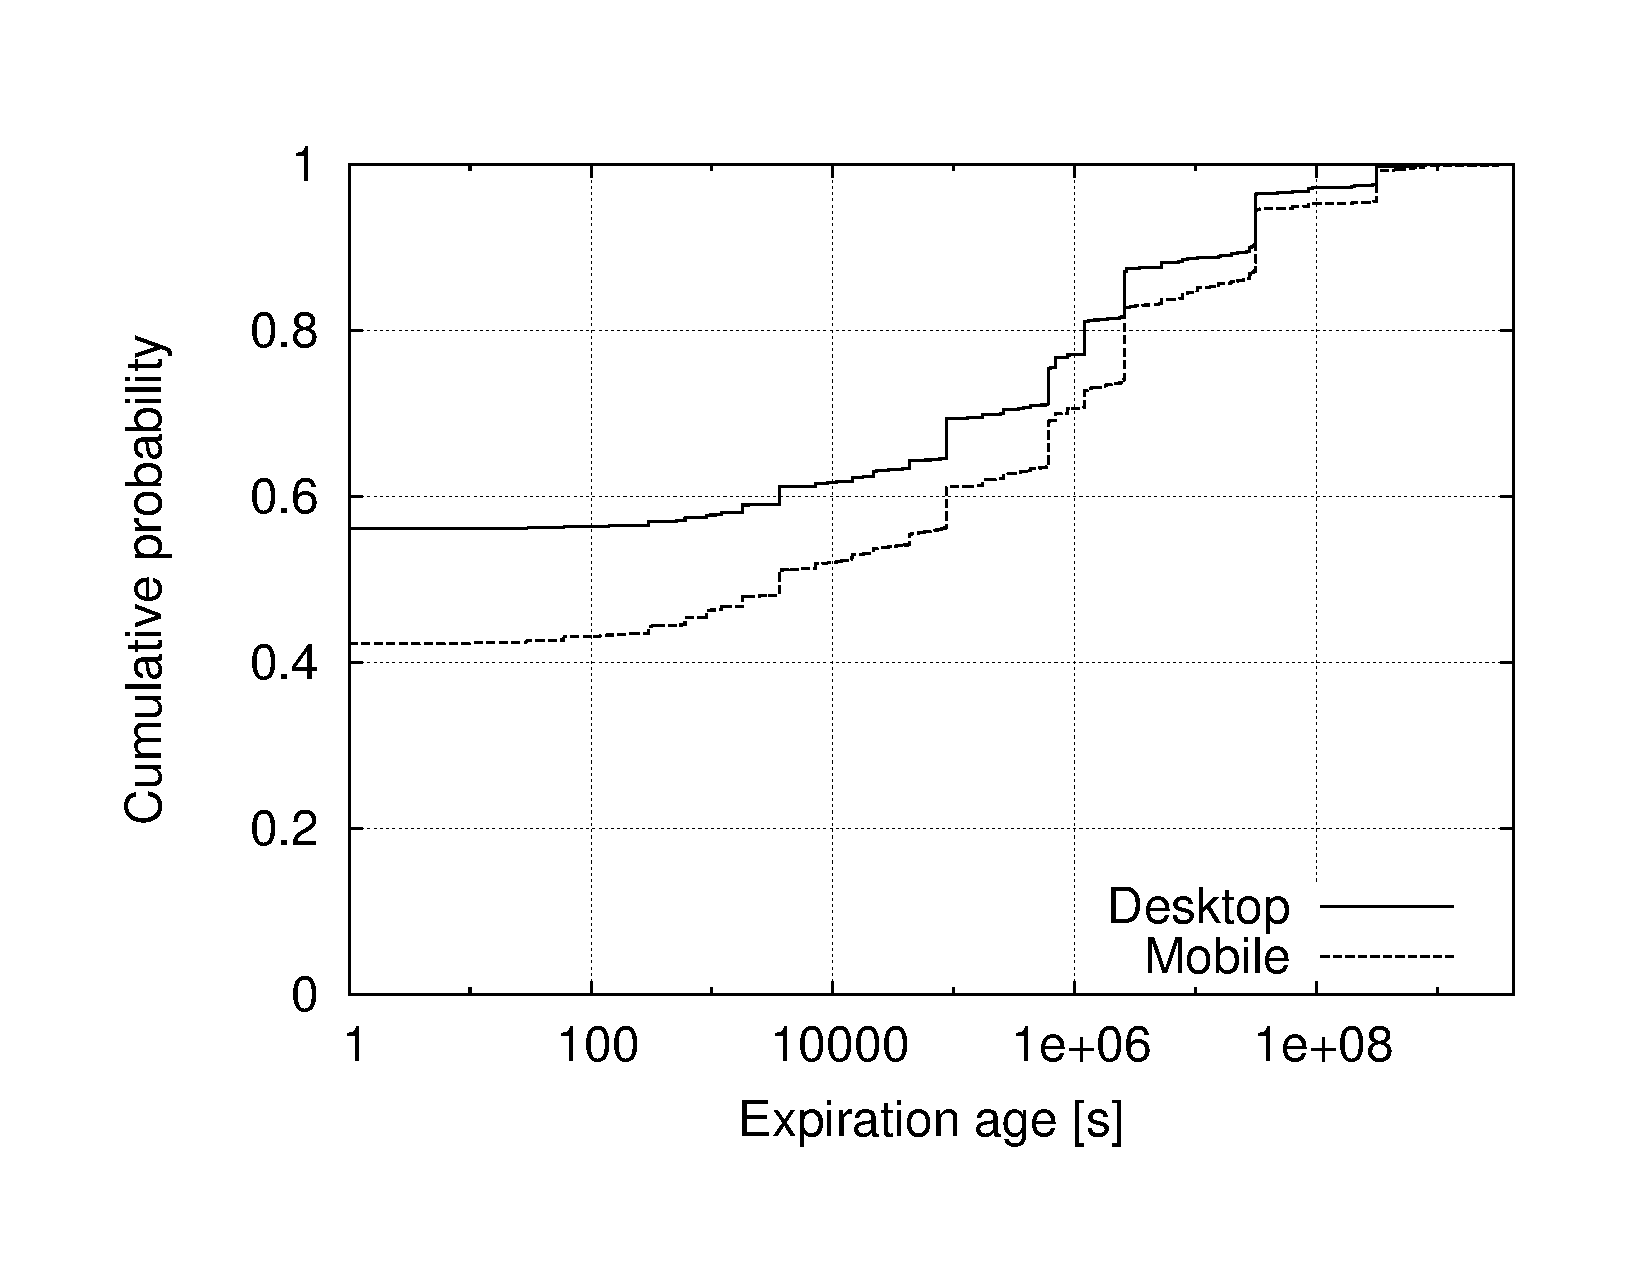
\includegraphics[scale=1,keepaspectratio,width=\columnwidth]{comp_cpd}
	\caption{Cumulative probability of expiration times for desktop and mobile responses.}
\label{fig:comp_cpd}
\end{figure}

We observe that a significant portion ($>40$ \%) of responses from web servers exhibits an immediate expiration and would, in turn, require an immediate retrieval by clients.
The cumulative expiration probability is higher for responses to desktop clients, which can be attributed to the typically more abundant bandwidth (and less optimization requirements) in contrast to a mobile setting (where web content developers might be more considerate of limitations).
In addition, we perform matching of request to mirror the individual example with a direction from desktop to mobile client. 

\subsection{Simulation Model Description}
\addcontentsline{toc}{subsection}{Simulation Model Description}
We evaluate the effectiveness of our approach through simulation, which we perform as follows.
For the time period of one week, we randomly select a web page from the mobile dataset and separate the data that is required to be downloaded and the data that is still available in cache due to the maximum expiration age of the individual objects. 
We subsequently wait for a random amount of time before repeating the procedure.

Initially, we sort all landing web pages $l, l=0,\ldots,L$ from the 
dataset based on their popularity ranking.
To simulate the popularity of web pages, it was found that the Zipf distribution effectively describes the popularity of individual requests.
We chose to utilize the non-modified Zipf distribution for our simulation purposes, noting that additional modifications to the distribution exist that can further enhance it, see, e.g., \cite{KrTeSh06}.
For the total number of web pages $L$, we derive the probability of page $l$ being selected in turn as
\begin{equation}
p(l)=\frac{l^{-\alpha}}{\zeta(l)},
\end{equation}
where $\zeta(\cdot)$ denotes the Zeta function. 
We furthermore set $\alpha=0.85$ as an average choice in common ranges utilized for this parameter.

Once the individual mobile web page $l$ was randomly chosen, we compare it to its desktop counterpart, with $\left\{ d,m \right\}$ denoting the request modality.
As each page $l$ exhibits a time-sensitive number of responses, we denote them as $r^{\left\{ d,m \right\}}(l,t)$ and each page exhibits $R^{\left\{ d,m \right\}}(l,t=0)$ in total.
Let $t_c(r^{\left\{ d,m \right\}}(l))$ denote the expiration or max-age directive received with the response at $r^{\left\{ d,m \right\}}(l,t=0)$.
The number of objects or responses to be retrieved at time $t$ in turn are given as 
\begin{equation}
R^{\left\{ d,m \right\}}(l,t) = \sum_{r^{\left\{ d,m \right\}}(l,0)} \left[ t_c(r^{\left\{ d,m \right\}}(l)) \ge t \right]
\end{equation}
where $\left[ \cdot \right] $ denotes the Iverson Bracket.
In the following, we abbreviate to $t_c$ for readability when in direct context.

We furthermore denote the size of the individual response retrieved at time $t$ as 
\begin{equation}
x_{r}^{\left\{ d,m \right\}}(l,t) = x_{r}^{\left\{ d,m \right\}}(l,0) \cdot \left[ t_c \ge t \right].
\end{equation}
The total size of objects or responses retrieved at simulation time $t$ thus is given as 
\begin{equation}
X^{\left\{ d,m \right\}}(l,t) =\sum_{r^{\left\{ d,m \right\}}(l,0)} x_{r}^{\left\{ d,m \right\}}(l,t).
\end{equation}


For performance evaluation purposes, we simulate the user behavior similar to the process outlined in~\cite{AnCoGrPa03}, whereby we randomly draw the time between requests $t_u$ as Pareto distributed using
\begin{equation}
p(t_u)=\beta k^\beta t_u^{-(\beta+1)},
\end{equation}
 with $\beta=1.5$, $k=30$.
We assume that no delays are accrued due to instantaneous cache retrievals or downloads. 
Using time index $i$, we thus derive $t_{i+1}=t_i + t_u$.
We continue the simulation until $t_{i+1} = t \ge T =  640800$ [s], i.e., one week.
To maintain tractability, we bundle the presented results into bins of 3600 seconds, i.e., one hour, through averaging.

\section*{Performance Evaluation Results}
\addcontentsline{toc}{section}{Performance Evaluation Results}
\label{s:results}

We present our results for the individual responses or web objects and the total number of bytes.
We note that through approximations, such as the ones described in Section~\ref{s:example}, an inference of energy consumption would be possible as well.
We perform the simulations with an average $\alpha=0.85$ for the utilized Zipf distribution and repeat each week-long evaluation 2000 times.
Initially, we present the total number of responses and bytes that would not require a download (i.e., would reside in the mobile cache) as a function of time in figures \ref{fig:simr_abs_reqs} and \ref{fig:simr_abs_byte}.

\begin{figure}
	\centering
	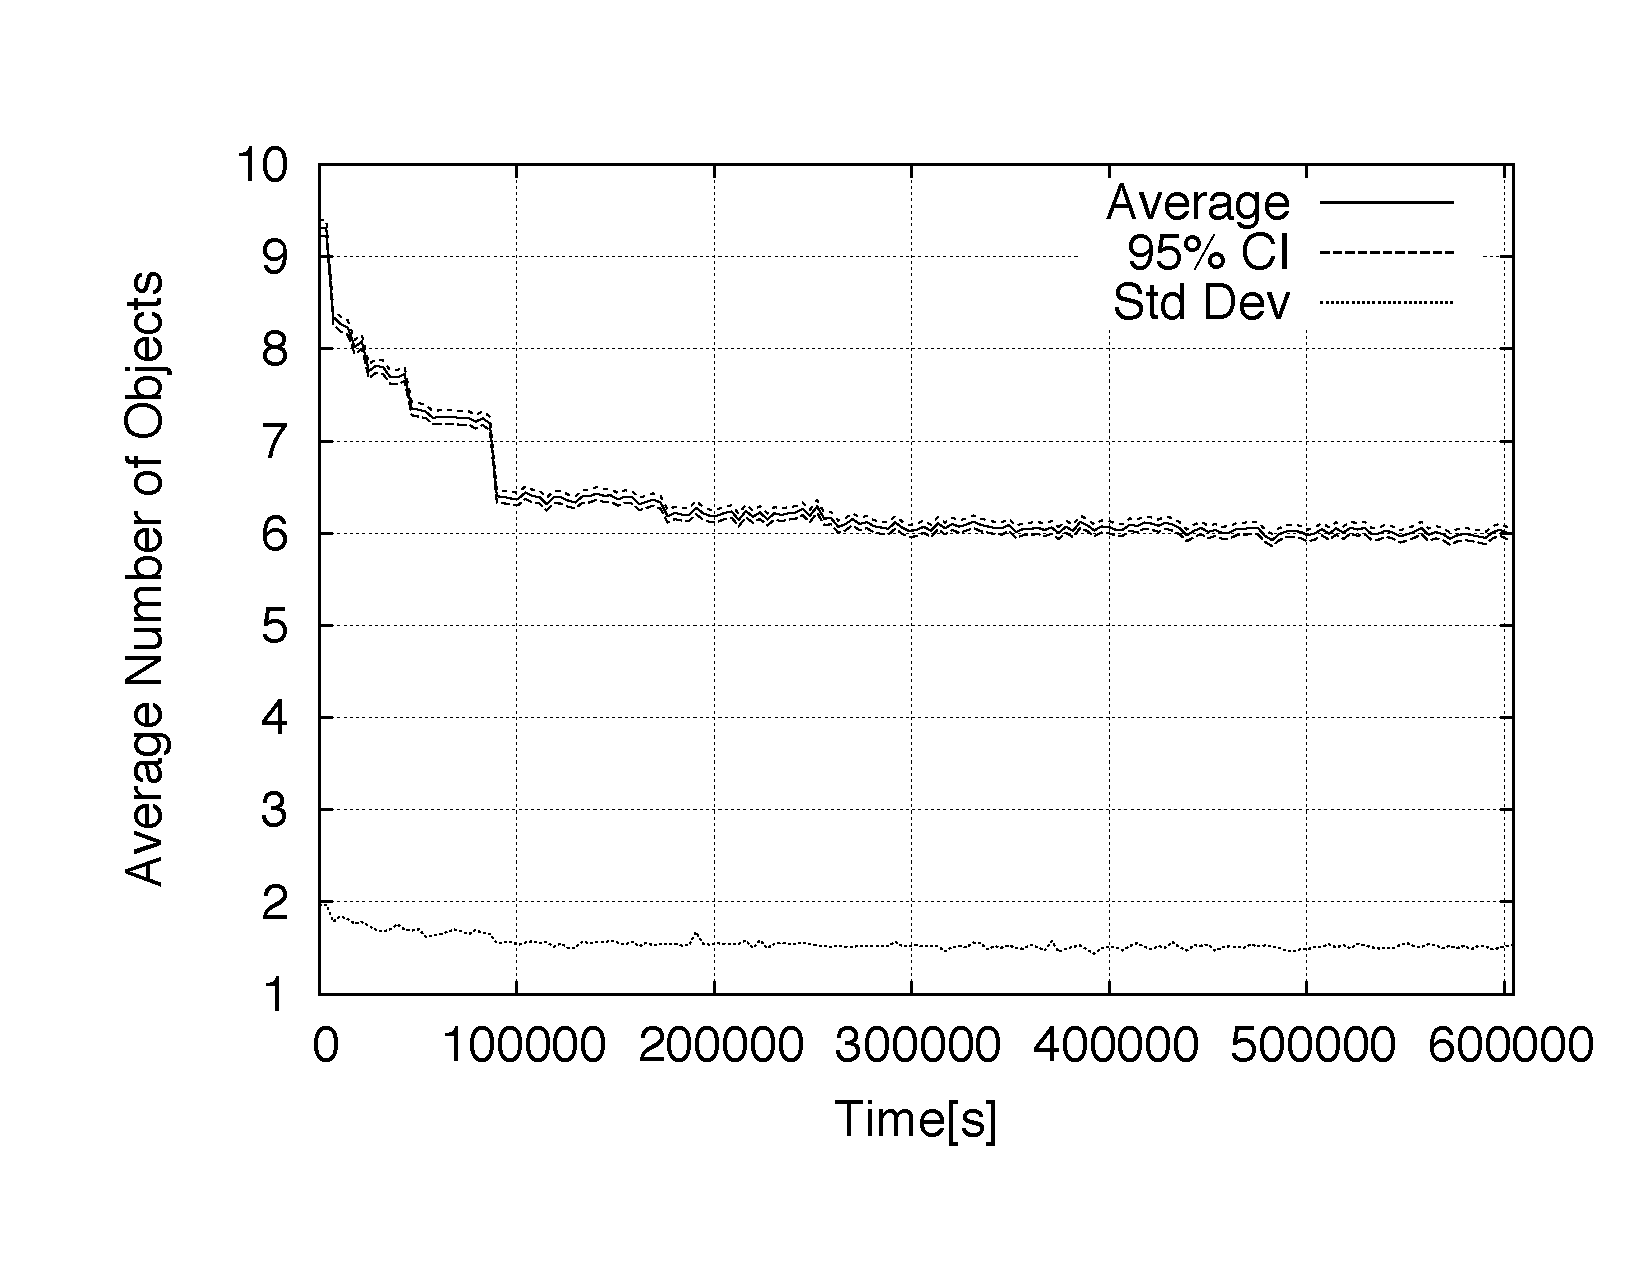
\includegraphics[width=\columnwidth]{Fig6-a}
	\caption{Simulation results for the number of responses that are in the transfered mobile device cache as averages in 1-hour bins..}
	 \label{fig:simr_abs_reqs}
\end{figure}

\begin{figure}
	\centering
	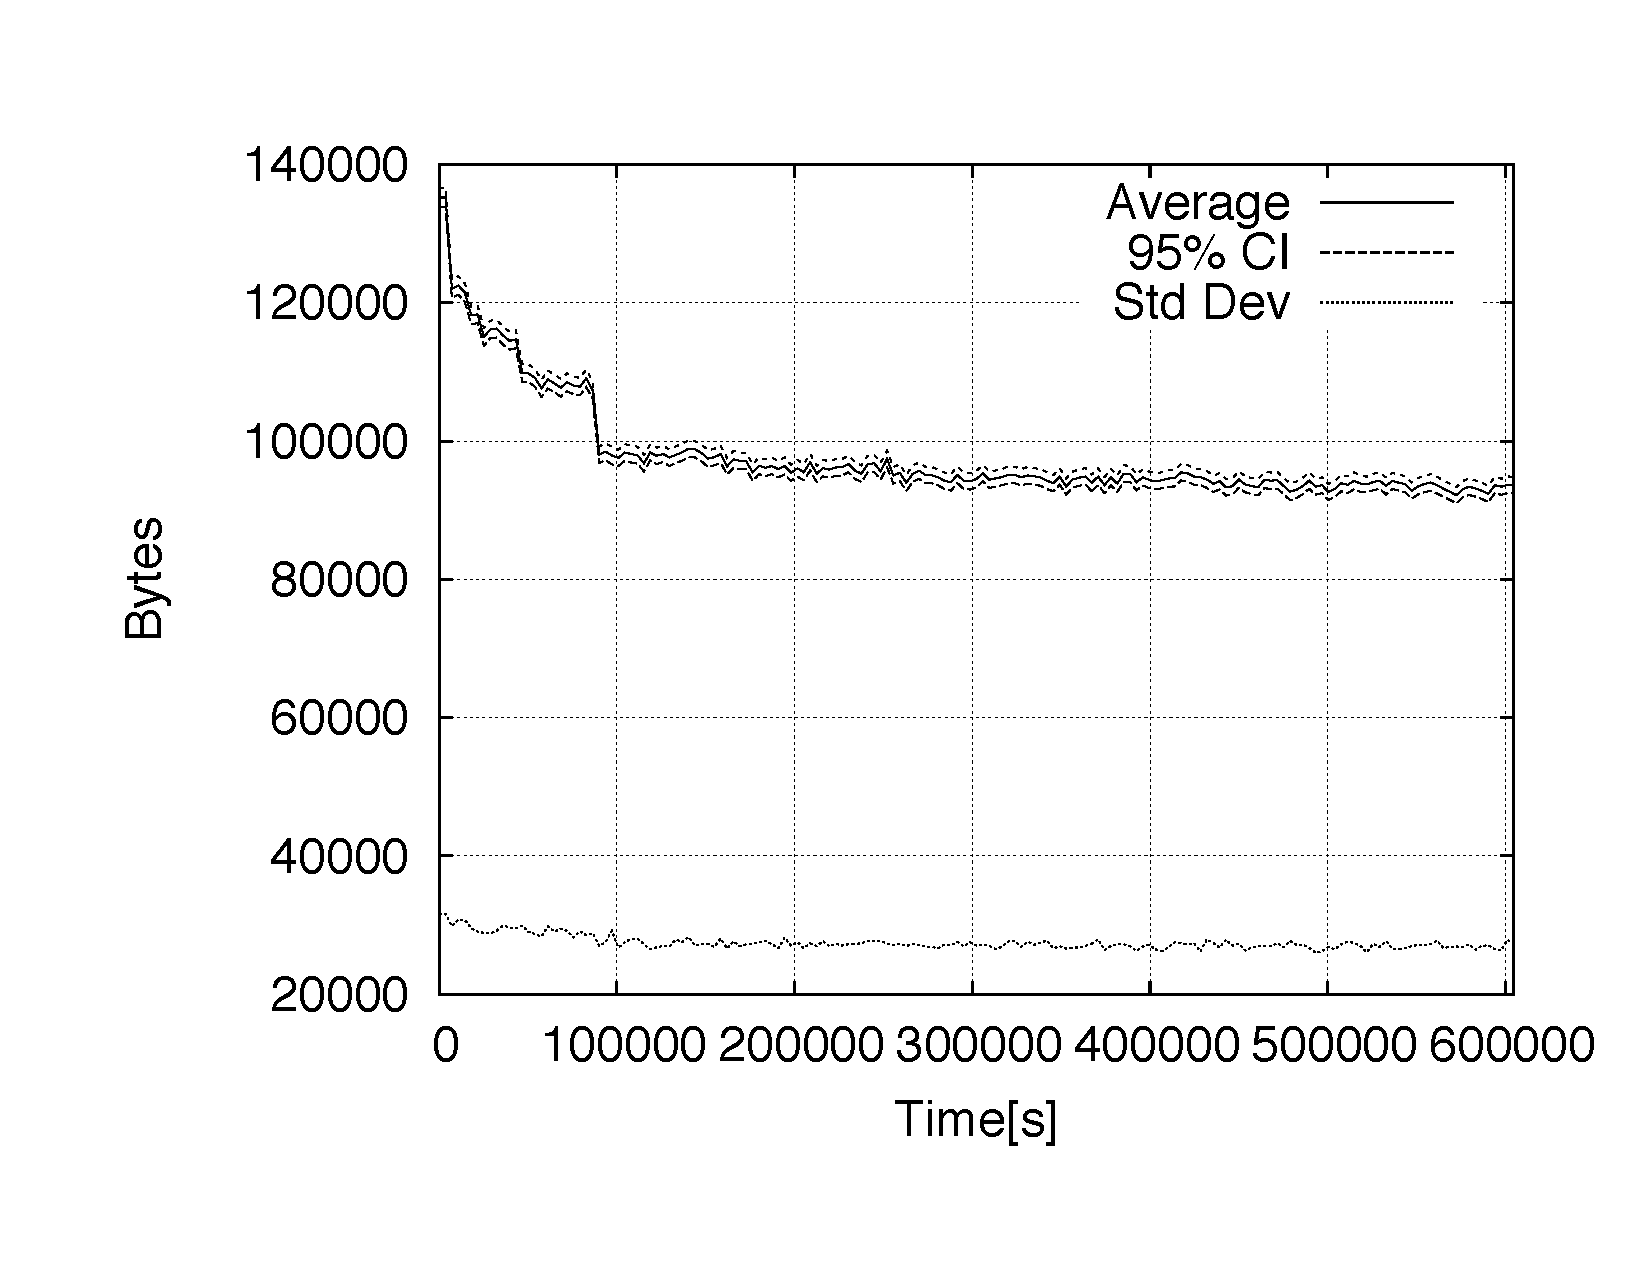
\includegraphics[width=\columnwidth]{Fig6-b}
	\caption{Simulation results for the attained savings for the number of bytes by transferring to the mobile device cache in 1-hour bins.}
	 \label{fig:simr_abs_byte}
\end{figure}

We note an immediate decrease in the number of requests, which is mirrored by the number of bytes as well (indicating a linear relationship as observed in, e.g., \cite{JoSe14Commag}).
We furthermore observe that the initial decline levels out at the simulation time of around one day, and  remains steady afterwards.
This indicates that within the simulation period of one week, initially a large number of items is non--shared between devices or exhibits no significant cache lifetime. 
In a following group of objects, cache lifetimes increase logarithmically, which leads to the exponential decline we observe here.
The narrow confidence intervals and low level of standard deviation indicate that the presented results are stable within simulation confines.

Next, we present how these findings translate into attainable savings with respect to requests for objects and bytes in figures \ref{fig:simr_sav_reqs} and \ref{fig:simr_sav_byte} in relationship to the total web page data without caching.

\begin{figure}
	\centering
	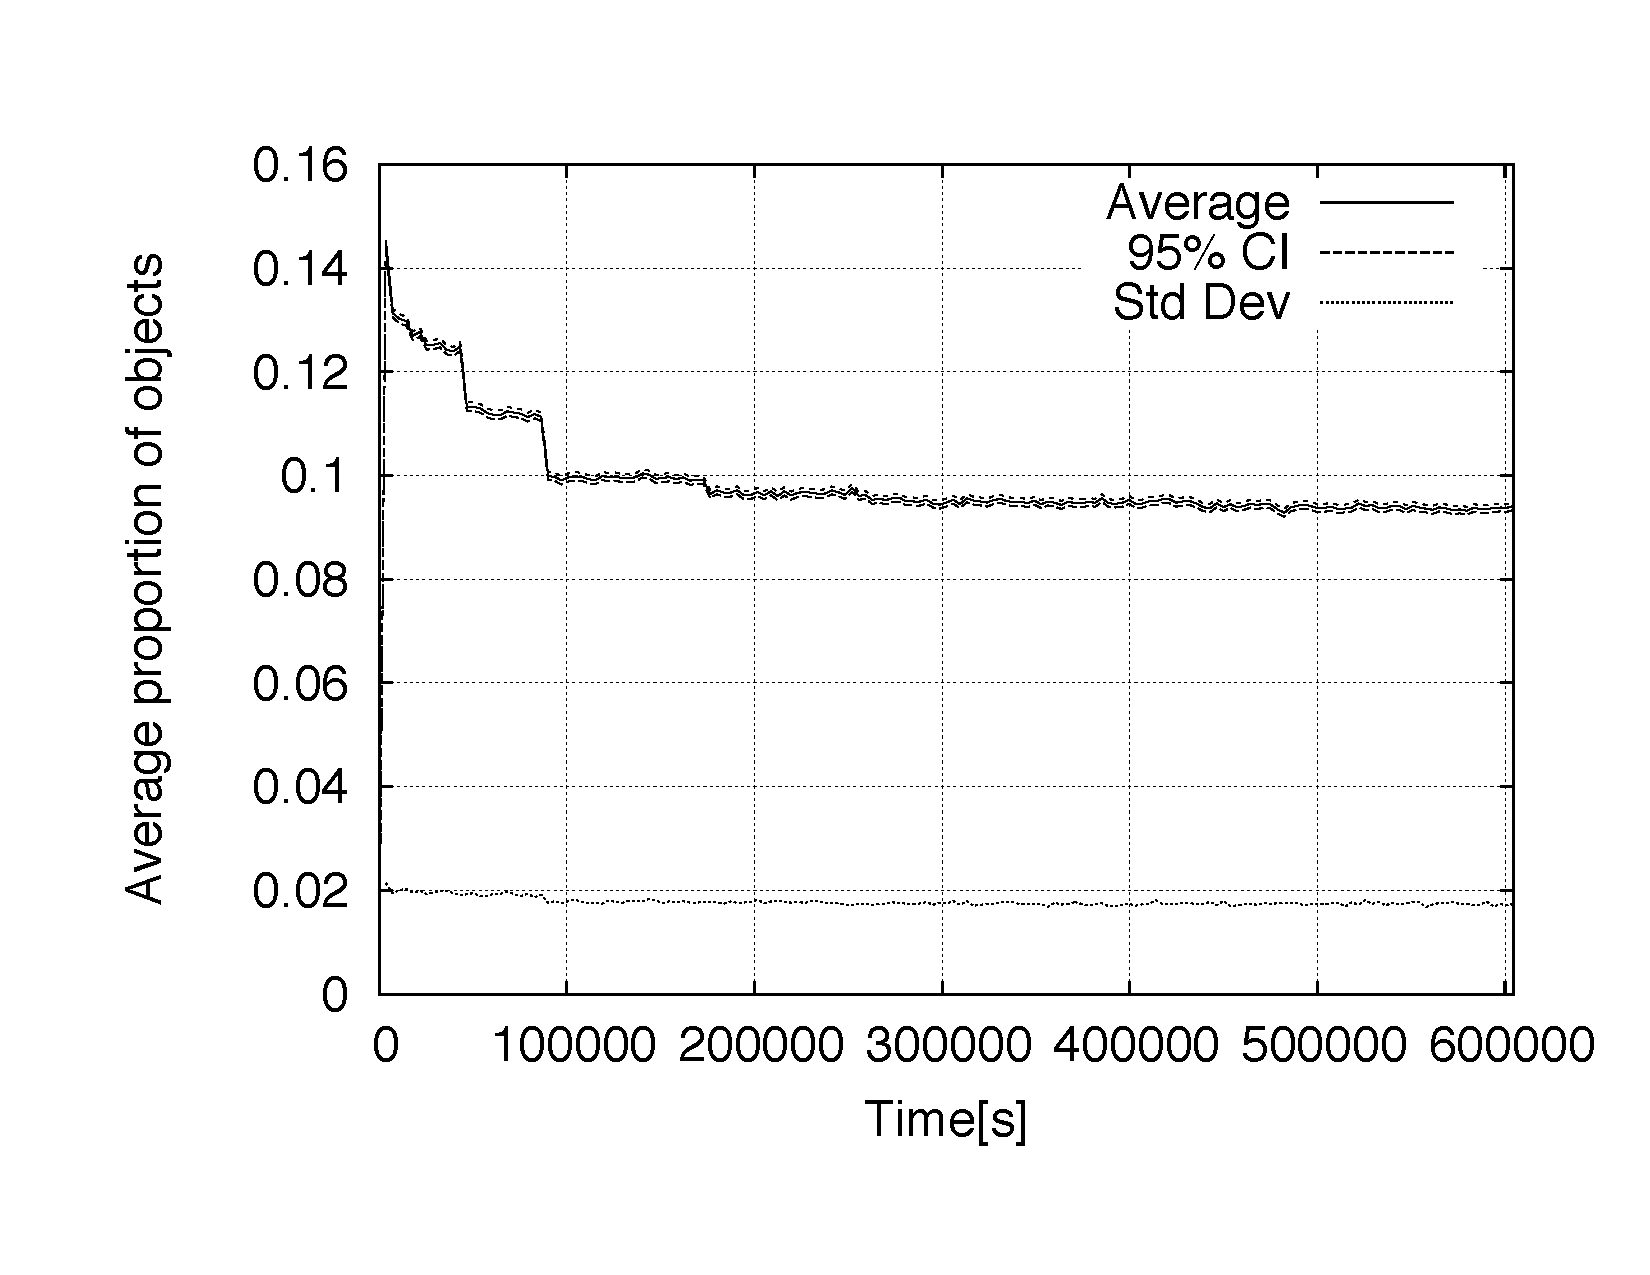
\includegraphics[width=\columnwidth]{Fig7-a}
	\caption{Simulation results for the attained savings for the number of requests by transferring to the mobile device cache in 1-hour bins.}
	 \label{fig:simr_sav_reqs}
\end{figure}

\begin{figure}
	\centering
	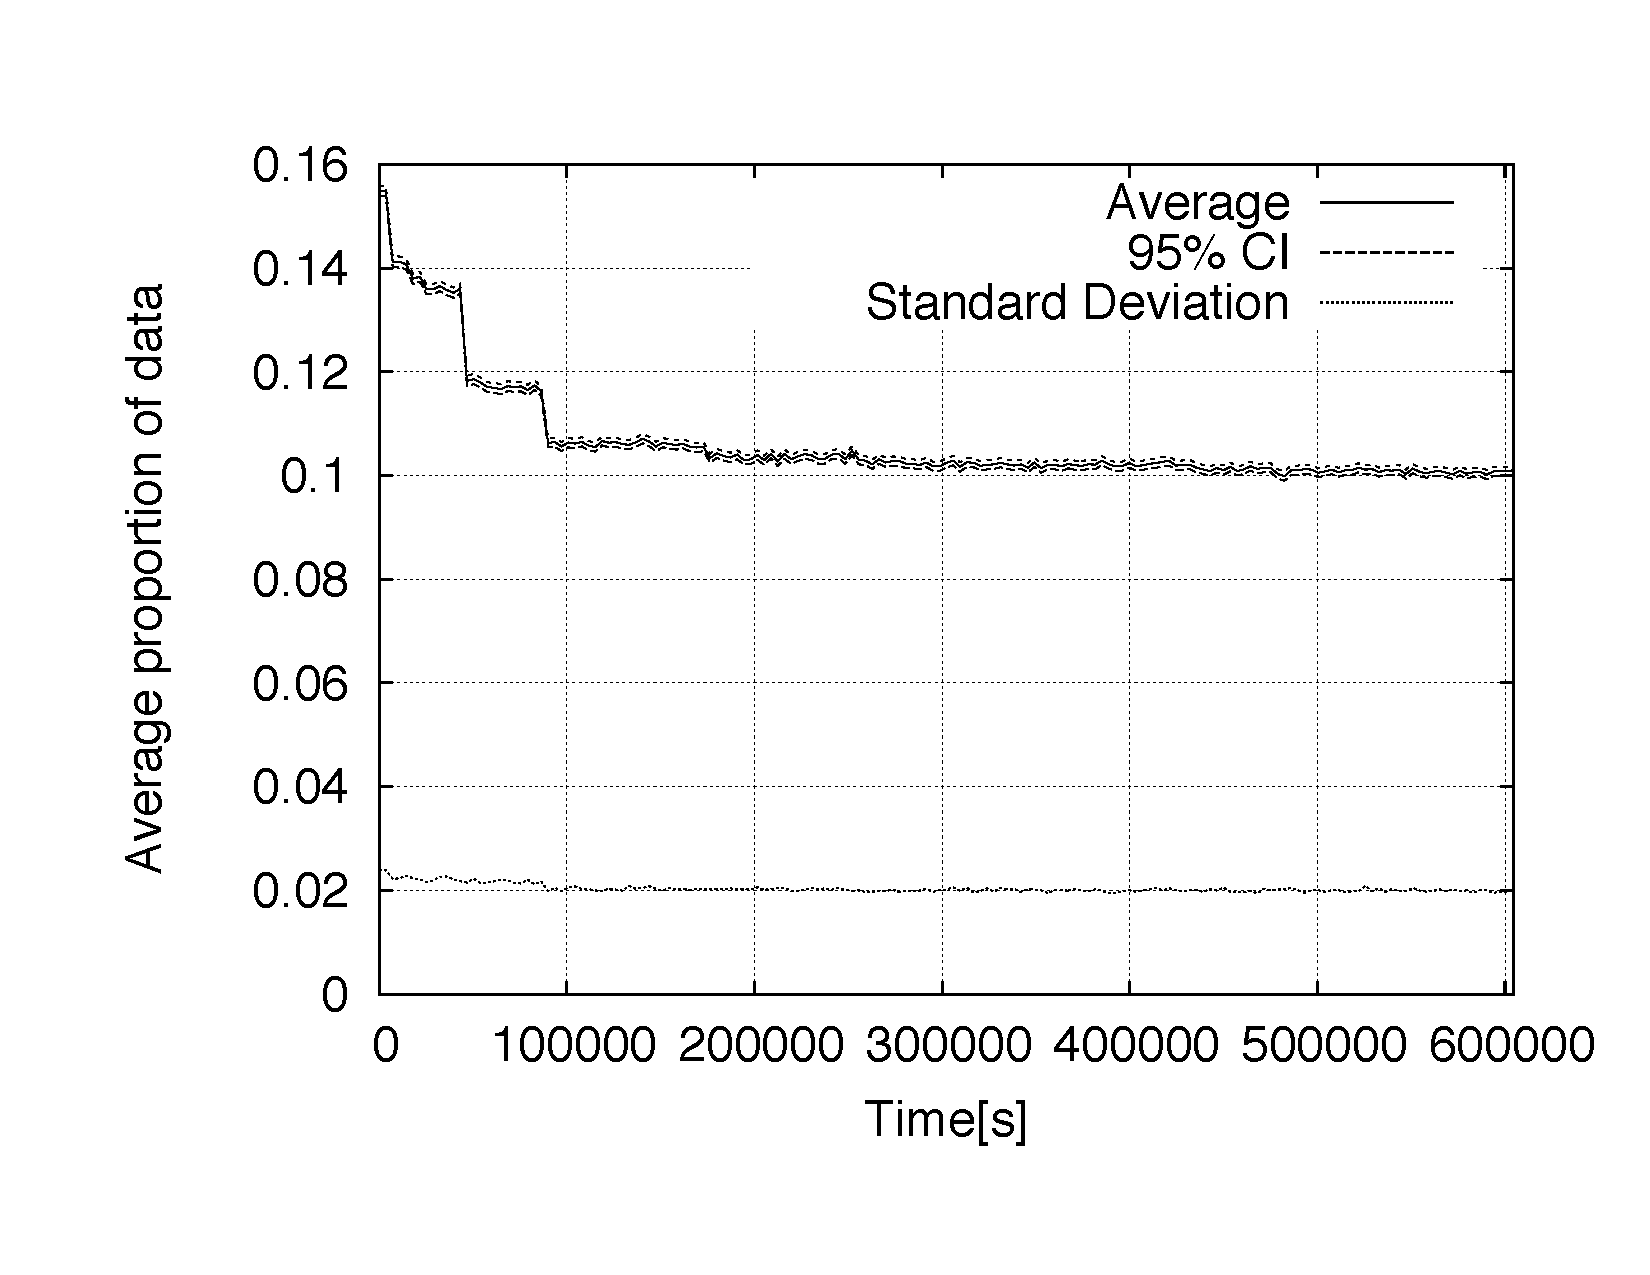
\includegraphics[width=\columnwidth]{Fig7-b}
	\caption{Simulation results for the attained savings for the number of bytes by transferring to the mobile device cache in 1-hour bins.}
	 \label{fig:simr_sav_byte}
\end{figure}

We initially note a declining trend similar to the one observed for the cached items in figures \ref{fig:simr_abs_byte} and \ref{fig:simr_abs_reqs}, but with more distinct ``jumps'' observable at half-day and day times of the simulation.
Overall, we note that almost 15 \% savings for objects and bytes decline to around 10 \% after the boundaries of a day (whereby objects exhibit lower levels and bytes exhibit higher levels).

To evaluate the impact of different web page popularity distributions, we present an evaluation of different $\alpha$ for the Zipf distribution in Figure~\ref{fig:sim3}, each with 500 simulation repetitions for $0.65 \le \alpha \le 1.05$.

We limit our comparison to bytes due to space constraints, noting that results obtained for objects are similar.
\begin{figure}[]
	\centering
	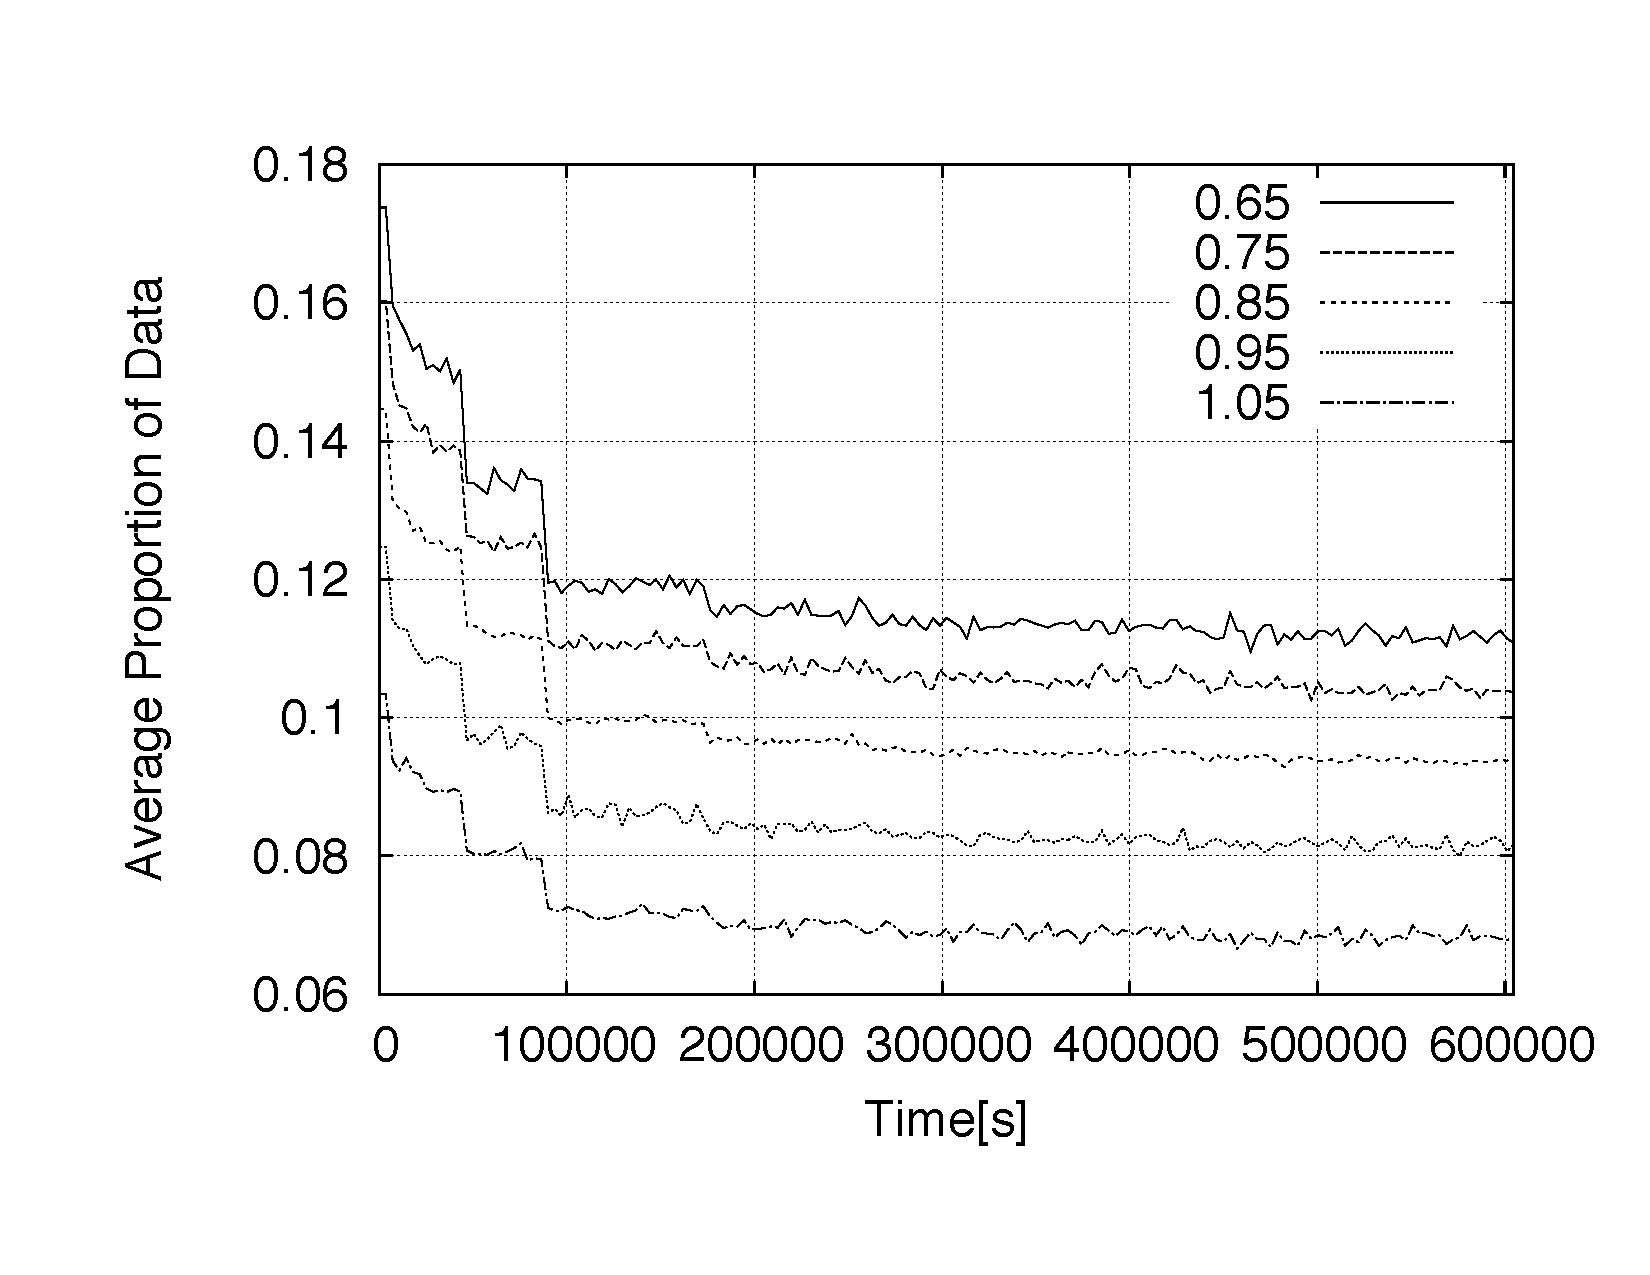
\includegraphics[width=\columnwidth]{Fig8}
	\caption{Average proportions of data in mobile cache for different Zipf distribution parameters $\alpha$.}
	\label{fig:sim3}
\end{figure}
We observe that all levels of $\alpha$ exhibit the same underlying trends, with slight and non-linear differences between levels.
We conclude that the distribution of web page popularity and the composition thereof has an overall impact on the long-term level of savings that can be attained.

Overall, we find a significant reduction in the required downloads for mobile clients that can be directly attributed to lower energy consumption levels and potential download latencies (and even costs for the mobile user through saved data transmissions).
Furthermore, this approach does not require sophisticated live evaluations, but only relies on cache forwarding to the mobile device.

\section*{Overnight Caching}
\addcontentsline{toc}{section}{Overnight Caching}

As an additional project, the possible power savings achievable through pre-caching contents of websites. Typically, most people tend to plug their mobile devices into a power source over night while they are sleeping. Also, many people tend to have Wi-Fi access in their homes, which can be accessible by the phone while the user is sleeping. Due to this, during the night or early morning, when a user is usually still sleeping, would be a great time for a mobile phone to go out and pre-cache the webpages a user visited the previous day since users are more likely to visit these same sites again the next day. By performing the pre-caching at night, the user would have the advantage of a power source and a Wi-Fi connection so they don’t drain their battery or data plan. As a result, they may also have faster load times throughout the day when they try to access the webpages since the webpages will already be cached locally on their mobile devices. This can also result in power savings since many of the items on the webpages may already be cached, so the mobile devices won’t have to make as many requests to go out and fetch as many of the required objects for a web page.

\subsection*{Simulation Set Up}
\addcontentsline{toc}{subsection}{Simulation Set Up}
To determine the overall potential savings we will simulate a 24 hour browsing session for a user. The two behavioral attributes of the user that we incorporate into the simulation model are the user think time and the webpage visited. User think time is the time in between page requests that a user spends viewing a web page before navigating to another webpage. The user think time is determined similarly to the process outlined in [4]. The user think time follows a Pareto distribution with $\beta$ = 1.5 and k = 30. Website popularity was shown in [5] to follow a zipf distribution with $\alpha$ = 0.85. So, to determine what webpage the user visits, an integer will be drawn from a zipf distribution with $\alpha$ = 0.85 and the webpage with the corresponding page rank will be the webpage that we simulate the user navigating to. The overall algorithm for simulating a 24 hour user browsing session can be seen below in algorithm \ref{alg:overnight_caching}.

\begin{algorithm}[H]
\label{alg:overnight_caching}
 \While{time < 86400 (1 day)}{
  Select webpage based on zipf distribution\;
  \If{expAge > time //Item hasn't expired}{
   AccumulateSavings()\;
   }
   time += Pareto($\beta$ = 1.5,k=30)\;
 }
 \caption{Algorithm for calculating savings and simulating a 24 hour user browsing session}
\end{algorithm}

\subsection*{Overall Cache Lifetime Behavior}
\addcontentsline{toc}{subsection}{Overall Cache Lifetime Behavior}

The overall lifetime of cache objects from mobile sites is shown in Figure \ref{fig:overall_bytes_over_24_hours}. Figure \ref{fig:overall_bytes_over_24_hours} depicts the total bytes remaining in cache over a 24 hour period. Roughly 35\% of bytes expire in cache almost immediately. Subsequently, there are also noticeable drops at periods of one hour, four hours, and twelve hours before slowly starting to level off to about 52\% of bytes remaining in cache after 24 hours. Figure \ref{fig:overall_responses_over_24_hours} depicts the total responses remaining in the mobile device’s cache over a 24 hour period. There is also a steep initial drop to about 55\% after the responses with an expiration age of zero expire. There are subsequent noticeable drops at periods of one hour, four hours, six hours, and twelve hours, before starting a steady decline to about 45\% of responses remaining in cache at the end of the 24 hour period.

\begin{figure}[]
	\centering
	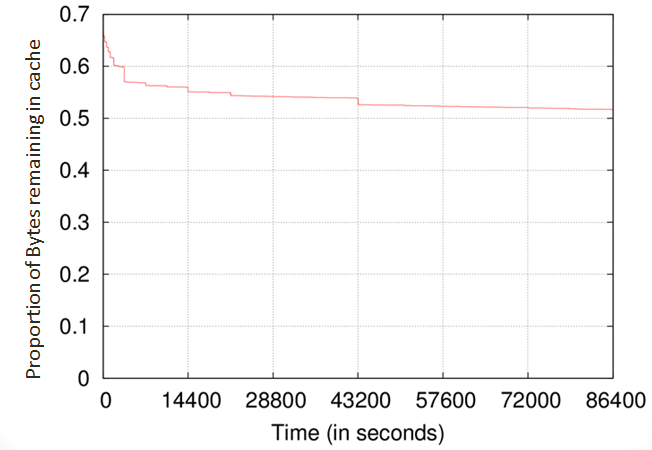
\includegraphics[width=\columnwidth]{overall_bytes_over_24_hours}
	\caption{The proportion of bytes remaining in cache over a 24 hour period.}
	\label{fig:overall_bytes_over_24_hours}
\end{figure}

\begin{figure}[]
	\centering
	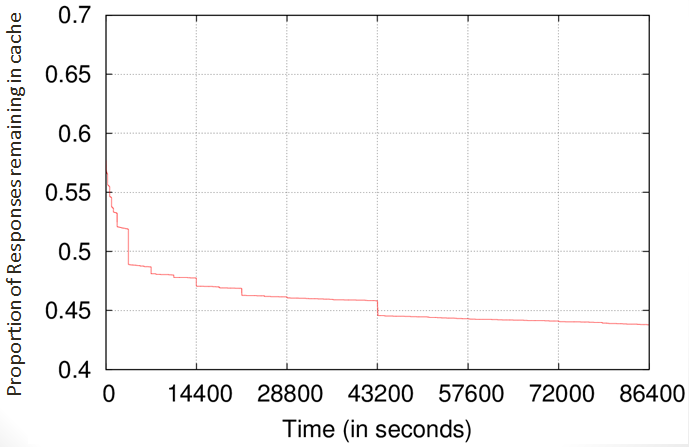
\includegraphics[width=\columnwidth]{overall_responses_over_24_hours}
	\caption{The proportion of HTTP responses remaining in cache over a 24 hour period.}
	\label{fig:overall_responses_over_24_hours}
\end{figure}

\subsection*{Results}
\addcontentsline{toc}{subsection}{Results}
We ran the simulation for two-thousand rounds to determine the possible savings along with their confidence intervals. The overall savings for a 24 hour period determined from our simulations seen be seen in Figure \ref{fig:simulated_bytes_remaining_in_cache_24_hours} and Figure \ref{fig:simulated_responses_remaining_in_cache_24_hours} along with their confidence intervals. In Figure \ref{fig:simulated_bytes_remaining_in_cache_24_hours}, after the initial drop from cache items with expiration ages of zero, the amount of bytes remaining in cache starts out at 43\% and starts to level off at about 35\% by the end of the day. The most significant visible drops occur at the two hour and twelve hour periods with other smaller noticeable drops throughout the day. Figure \ref{fig:simulated_responses_remaining_in_cache_24_hours} depicts the total proportion of responses remaining in cache over a 24 hour period along with the 95\% confidence intervals. After the initial drop from cache items with expiration ages of zero, the proportion of responses remaining in cache starts out at about 37\% and levels off to about 30\% by the end of the day. As expected, the most visible drops are in similar locations as Figure \ref{fig:simulated_bytes_remaining_in_cache_24_hours}, at the two hour and twelve hour periods with other smaller noticeable drops throughout the day.

\begin{figure}[]
	\centering
	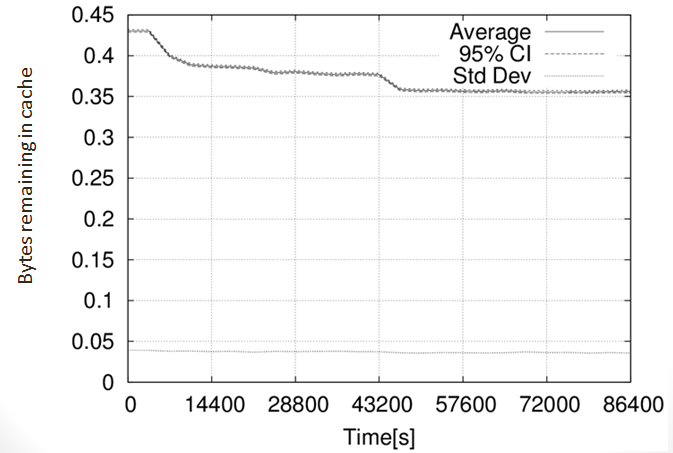
\includegraphics[width=\columnwidth]{simulated_bytes_remaining_in_cache_24_hours}
	\caption{The proportion of bytes remaining in cache over a 24 hour period using our simulation model.}
	\label{fig:simulated_bytes_remaining_in_cache_24_hours}
\end{figure}

\begin{figure}[]
	\centering
	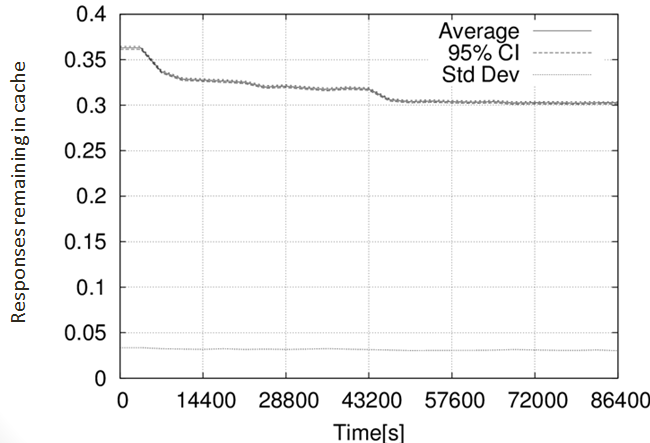
\includegraphics[width=\columnwidth]{simulated_responses_remaining_in_cache_24_hours}
	\caption{The proportion of HTTP responses remaining in cache over a 24 hour period using our simulation model.}
	\label{fig:simulated_responses_remaining_in_cache_24_hours}
\end{figure}

\section*{Conclusion}
Performance Evaluation Results
\label{s:conc}
We exemplarily evaluated the content of modern web pages and the identical objects that can be found when requesting the same web page from different devices with different display modalities, such as desktop and smartphone.
Assuming mobile users visit the same pages on their mobile device that they visit on their desktop computer as well, we simulated the access of landing web pages and evaluated the potential for cache forwarding.
Our basic approach is able to save upward of 7.5 \% of mobile request or bytes even for very distant time horizons.
In the more typical daily time range, our approach can yield almost linearly decreasing savings stating at about 14 \%, without requiring any sophisticated prediction mechanisms, but only a direct cache transfer.
We note that similarly, exchanges between mobile and fixed devices belonging to a user are possible, including keeping a cloud-based reference of pages that a user visits (similar to Google Chrome's synchronization features).
\chapter{Desktop and Mobile Web Page Comparison: Characteristics, Trends, and Implications}

\section*{Introduction}
\addcontentsline{toc}{section}{Introduction}

The broad proliferation of web-based services and the trend to outsource formerly server-based and/or locally maintained services into ``the cloud'' have significantly altered the manner of web page designs and compositions.
As the nature that underlies a typical web page changed over time, so have their characteristics and resulting implications for the networks that transport them.
In turn, a plethora of popular applications and interactions that are performed by users are enabled by using web-based services and have fueled the growth of Internet traffic.

Popular past web characteristics, model usages, and performance analysis approaches, see, e.g., \cite{BaCr98} or, more recently, \cite{LiZhZhChGr10}, do  not necessarily reflect the current state of the World Wide Web anymore.
While Cisco, Inc. predicts that video will account for the largest portion of networked traffic (and its growth) in the near future~\cite{Ci13}, consumer-based web traffic is forecasted to exponentially increase during the same time frame as well, putting an overall burden on access networks.

Longitudinal studies have recently emerged that target capturing the dynamic behavior of the World Wide Web over time, such as \cite{CaAlPa10}.
In~\cite{IhPa11}, the authors investigate five years (2006-2010) of fixed web site traffic captured through a proxy system and found significant impacts as a result of interactions.
Furthermore, they note that the overall loading time of web pages has been reduced due to higher levels of caching and an increase in concurrent connections made by desktop browsers.
Similarly, the complexity of web sites was evaluated in~\cite{BuMaSe11,BuMaSe13}. The authors found that the number of objects that were loaded (independent from their relative location) has the highest impact on web page load times.
Interestingly, the authors additionally found that for their dataset, ($i$) non-landing pages tended to be less complex and ($ii$) mobile web pages tended to be of lesser complexity.


The broad proliferation of mobile devices that can connect to Internet-based services has given rise to considerable amounts of data that are exchanged with web-based services. 
Several predictions indicate that there will be a continuous increase in the demand for mobile data, see, e.g. \cite{Ci13}, and that access to web-based services will soon be mainly performed through mobile devices.
While the outlined recent studies and ongoing works mainly investigate the traditional desktop-based web access, the emergence of mobile web access gives rise to a new set of problems that are direct derivatives of the characteristics of mobile devices.
In a recent overview of the battery impact that different web page elements have on the power consumption of mobile devices, Java Script and CSS were identified as the main contributors to the power consumption during rendering, see~\cite{ThAgNiBoSi12}.
In addition to the complexity of web pages, their composition can have a direct impact on the web-related performance of mobile devices.

Our contribution fills the currently existing gap of an in-depth evaluation of the trends that emerge for desktop and mobile client versions of web pages, for which we cover the time period from mid-2011 to the end of 2013.
We demonstrate the similarities and disparities of the current fixed and mobile web and outline overall notable characteristics and trends that web page developers as well as networking researchers and practitioners should consider in their respective optimization efforts.

The remainder of this paper is organized as follows. 
In the next section, we describe the underlying dataset from httparchive.org and how we processed it.
Subsequently, we compare the characteristics for desktop and mobile clients with respect to web page objects, sizes, and caching in Section~\ref{s:compare}.
We discuss the results and implications in Section~\ref{s:discuss} before we conclude in Section~\ref{s:conc}.



\section*{Data Set and Pre-Processing}
\addcontentsline{toc}{section}{Data Set and Pre-Processing}
\label{s:dataset}
In this paper, we utilize the \url{httparchive.org}~\cite{ht13} publicly available dataset of captured web performance metrics. 
As an industry-supported project, its goal is to provide ``a permanent repository of web performance information such as size of pages, failed requests, and technologies utilized.''
The overall starting points are the initial client view statistics, i.e., non-cached web page views, that are gathered by the httparchive.org projects at the beginning and in the middle of each month.
We illustrate the overall process in Figure~\ref{fig:setup}.
\begin{figure}
	\centering
	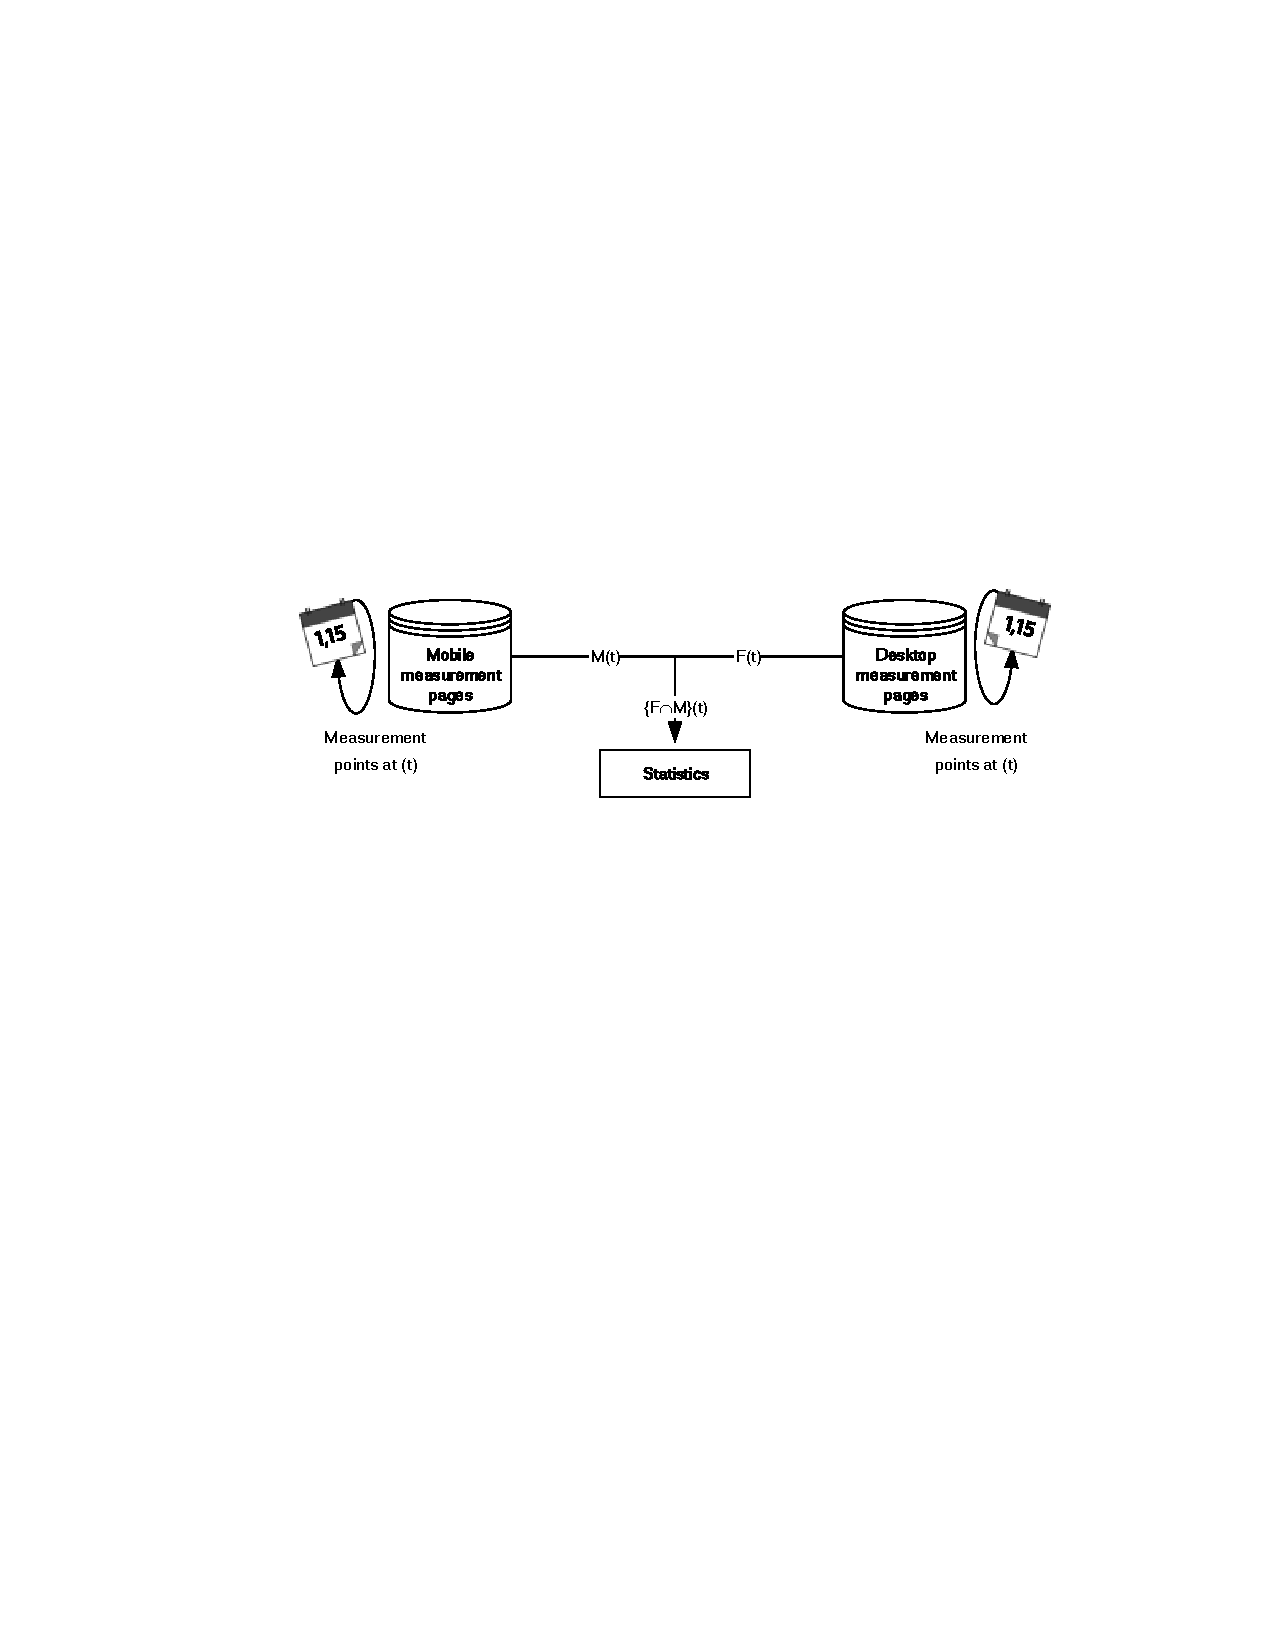
\includegraphics[width=.45\textwidth]{setup}
	\caption{Approach for gathering the general statistics evaluated in this contribution: based on the original archives, we compare the fixed and mobile web pages contained in each bi-monthly measurement and evaluate only those that can be found in desktop and mobile web page requests to allow for a direct comparison.}
	\label{fig:setup}
\end{figure}
As with any project that has to evolve over time to account for changes in technologies, some underlying measurement setups have to change over time as well.
In the remainder of this section, we describe the initial gathering and processing of this dataset in greater detail.


\subsection*{General Notes}
\addcontentsline{toc}{subsection}{General Notes}
As we utilize the measurements over a significant amount of time from June 1, 2011 to December 15, 2013, we initially note that some of the underlying measurement configurations have changed over time, which includes multiple facets, such as Unique Resource Locators (URLs), browser versions, connection speeds, or incorporation of `lazy loading' of resources.
We reason that overall, however, the changes made were reflecting industry trends as well as personal connectivity trends (such as modified access network speeds) and can be seen as representative of the typical connection scenarios for the World Wide Web.
We refer the interested reader to the online documentation of the \url{httparchive.org} project for more details pertaining to the measurement setup used and detailed information about changes.

\subsection*{Web Page Selection and Processing}
\addcontentsline{toc}{subsection}{Web Page Selection and Processing}
We select the available page statistics for both desktop (fixed) and mobile web pages over the range of more than two years; the available points in time are at the beginning and the middle of each month.
This results in a total of 62 datasets each for fixed and mobile web clients, respectively.
The evaluation by the httparchive.org project used the Apple iPhone's built-in browser client for mobile requests and the Microsoft Internet Explorer browser client for desktop requests (represented by different user agent strings in the HTTP requests sent).
We initially determine all web sites that are common for both archives, i.e., web sites that for each measurement time were evaluated for both, fixed and mobile clients, to allow for a comparative evaluation of their described metrics.
This results in a fair comparison at each individual measurement point, but yields an initial reduction of the total number of web pages that we compare. We note, however, that there are more than 900 pages in the initial (smallest) set. 
For each of the measurement times, we subsequently aggregate the measured web page characteristics over all web sites that were selected in a particular client role -- as a result, we derive a representative average snapshot of the characteristics that make up ``the web'' as accessed using different web clients over time.
In addition to the time-varying selection of web pages, we compare the web pages that are found for desktop and mobile clients throughout the longitudinal evaluation time period, which results in a smaller subset of 46 web pages.


\subsection*{Time Variability of the Dataset}
\addcontentsline{toc}{subsection}{Time Variability of the Dataset}
The underlying dataset that we utilize has undergone changes over time. 
Specifically, the base URLs that comprise the original dataset from httparchive.org (i.e., before we match fixed and mobile pages at each measurement point) were changed, namely ($i$) by switching to the Alexa top 1000000 web sites in November 2011 and ($ii$) by increasing the number of URLs evaluated in September 2012, see~\cite{ht13}. Other changes that were performed are more network-level oriented and should have a lesser impact on the static results we report here.
To evaluate how these changes impact the diversity of values encountered in the dataset over time, we employ the entropy of the Theil population, which is itself based on the Theil index~\cite{Th72}.

Specifically, we evaluate the number of web requests and the total number of bytes for each request type over time, as we are more interested in the overall quality of the selected data subset (i.e., statistics for pages that can be found in both datasets).
We illustrate the result as function of time in Figure~\ref{fig:theil}, whereby we initially note that higher values represent a higher diversity of the underlying dataset (Theil population).
\begin{figure}[t]
	\centering
	\subfloat[Number of requests per page]{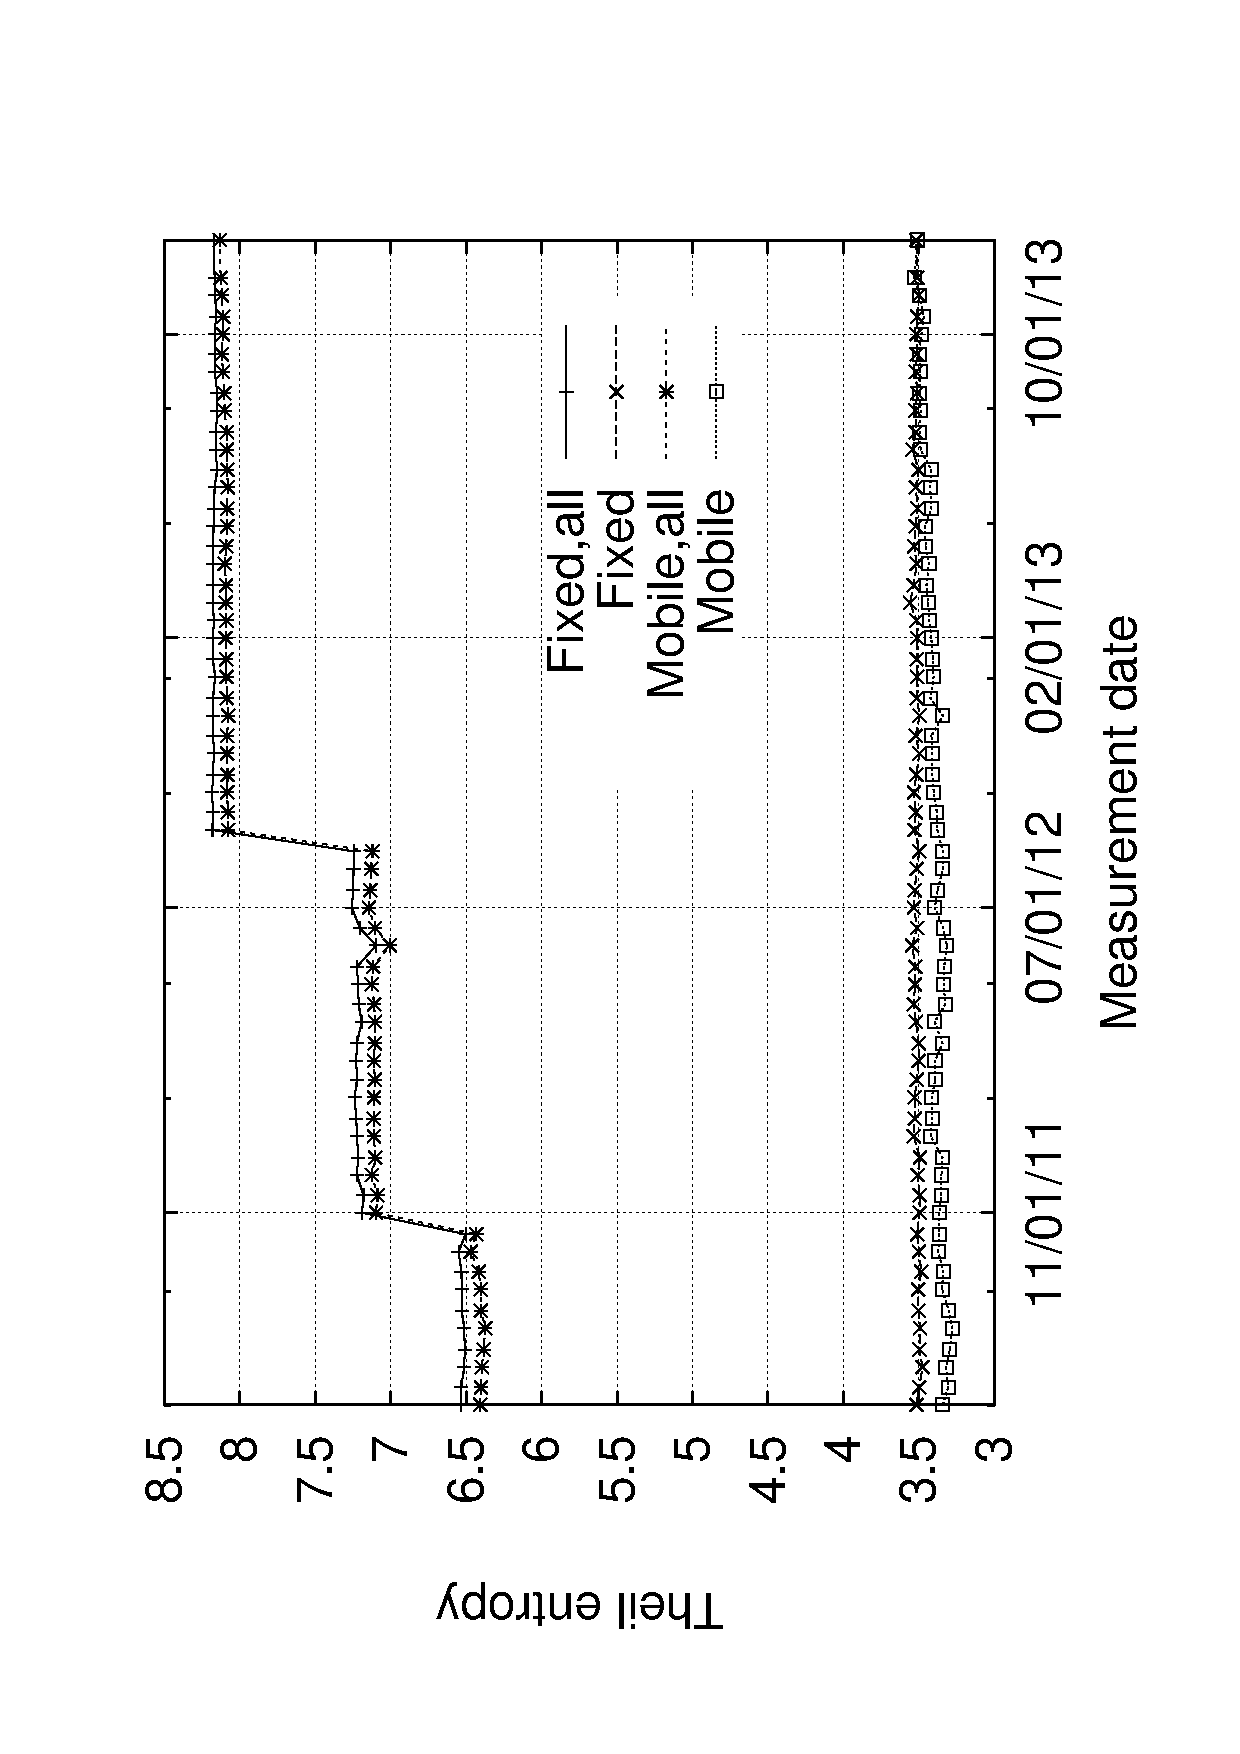
\includegraphics[width=.45\textwidth]{theil_reqs}}\qquad
	\subfloat[Number of bytes per page]{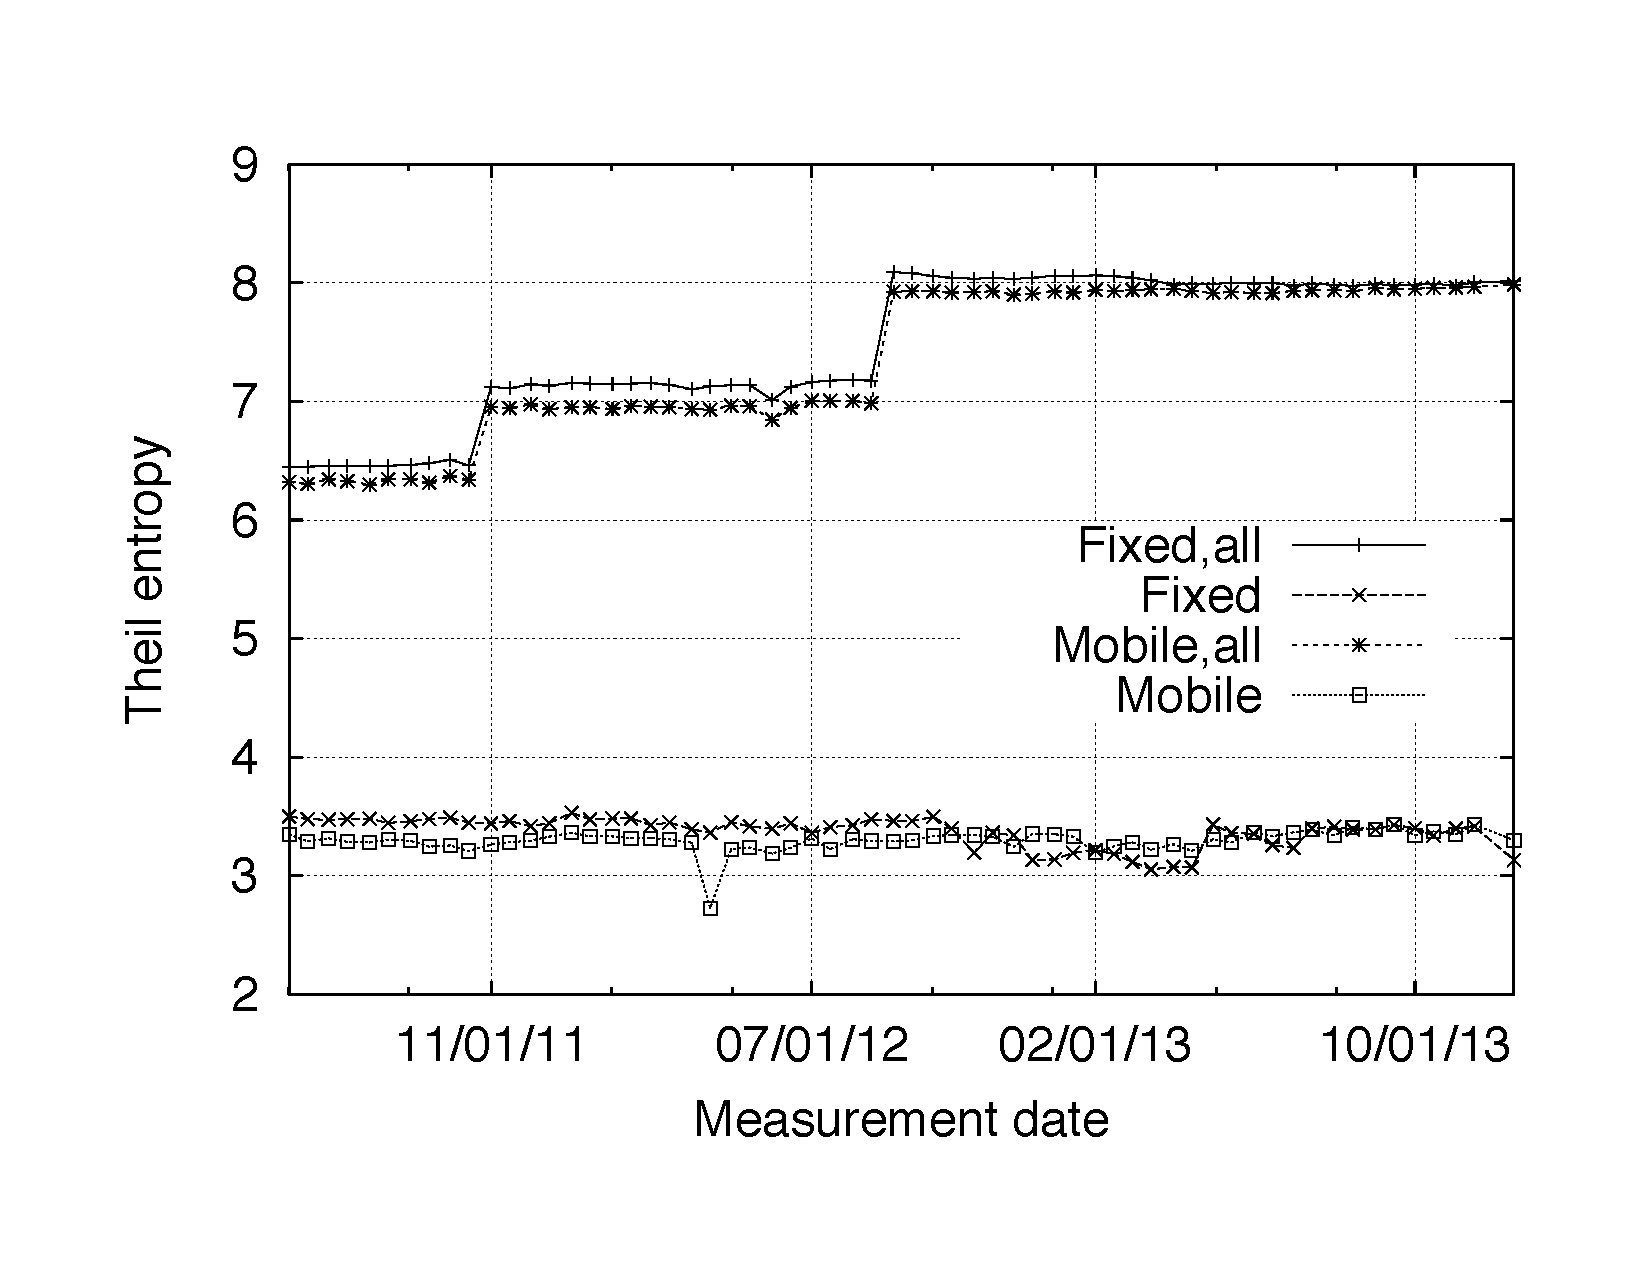
\includegraphics[width=.45\textwidth]{theil_bytes}}
	\caption{Theil entropy for the number of objects requested and the number of bytes for web pages present in the httparchive.org's desktop and mobile client data files for all pages at each measurement point (all) and the subset of continuously included pages.}
	\label{fig:theil}
\end{figure}
We observe that the entropy curves for each of the selected features (requests, bytes) are fairly close for each of the two modes (fixed, mobile), with significant ``jumps,'' i.e., changes of their overall level, at two distinct measurement points for the larger dataset.
These ``jumps'' occur at times where the underlying number and source set of the httparchive.org base URLs were changed, as outlined above.
We note that these changes, however, affect all client modes and type of characteristics evaluated in a similar manner by significantly increasing the diversity of measurement results, which is immediately visible from Figure~\ref{fig:theil}.
For the smaller subset, we observe a more steady behavior, with only small deviations and outliers over the entire measurement time period.
Overall, we note that the Theil entropy levels for the desktop client values are slightly higher than their mobile client counterparts; however, they remain within close range.
This closeness in the calculated Theil entropy additionally motivates us to focus on the overall averages of the values we compare in the remainder of this paper.


\section*{Comparison of Desktop and Mobile Web Page Characteristics}
\addcontentsline{toc}{section}{Comparison of Desktop and Mobile Web Page Characteristics}
\label{s:compare}
In this section, we compare the average values we obtained from the joint httparchive.org datasets for the desktop and mobile web client versions of the same set of web pages requested, as given by their URLs.

\subsection*{Average Number of Web Site Objects}
\addcontentsline{toc}{subsection}{Average Number of Web Site Objects}
\label{ss:objects}
Initially, we investigate the average number of objects requested when accessing a web page for the first time and illustrate the results in Figure~\ref{fig:requests} for both client types and all web pages compared to the subset present throughout all measurement points.
\begin{figure}
\centering
	\subfloat[Average requests for desktop and mobile client versions.]{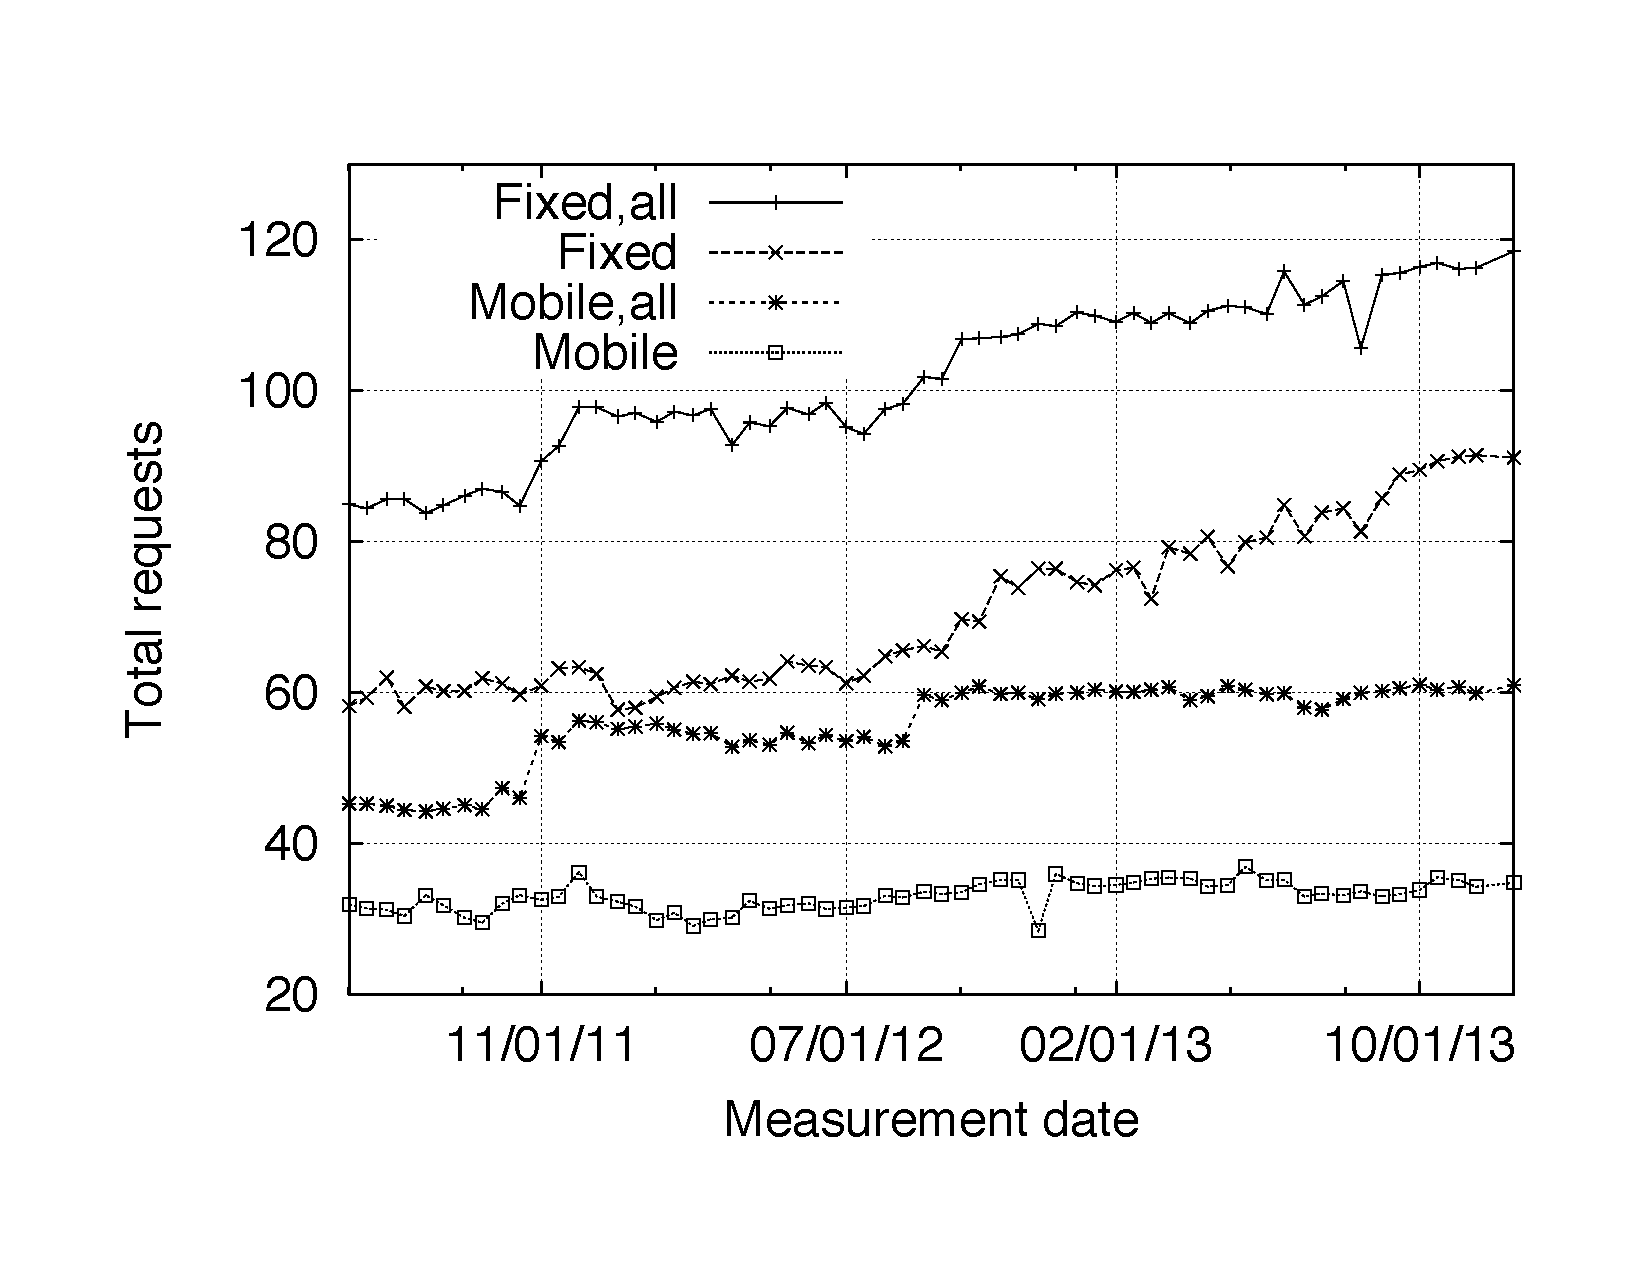
\includegraphics[width=.45\textwidth]{totalRequests_all}}\\ 
	\subfloat[Categorized requests for desktop client (all pages).]{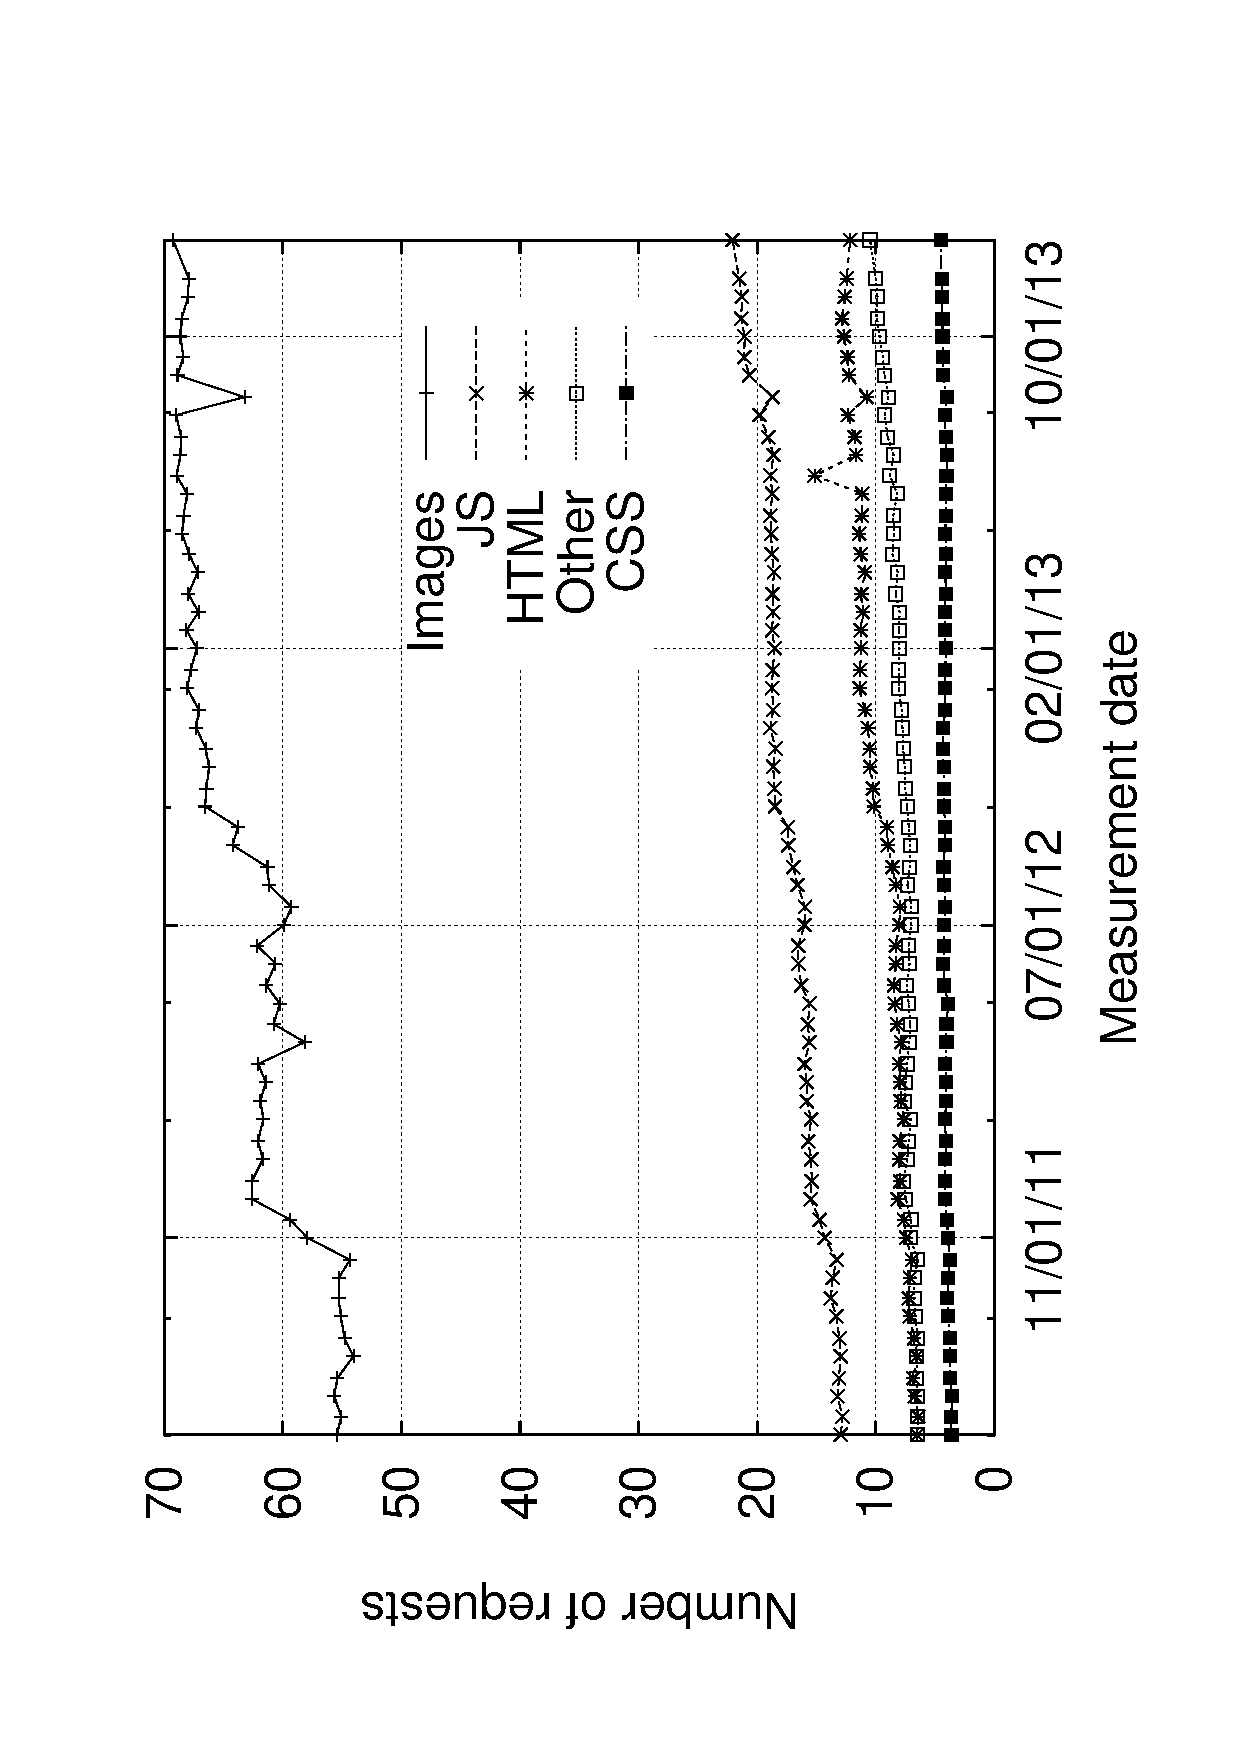
\includegraphics[width=.45\textwidth]{req_by_type_fixed_all}}\qquad
	\subfloat[Categorized requests for mobile client (all pages)]{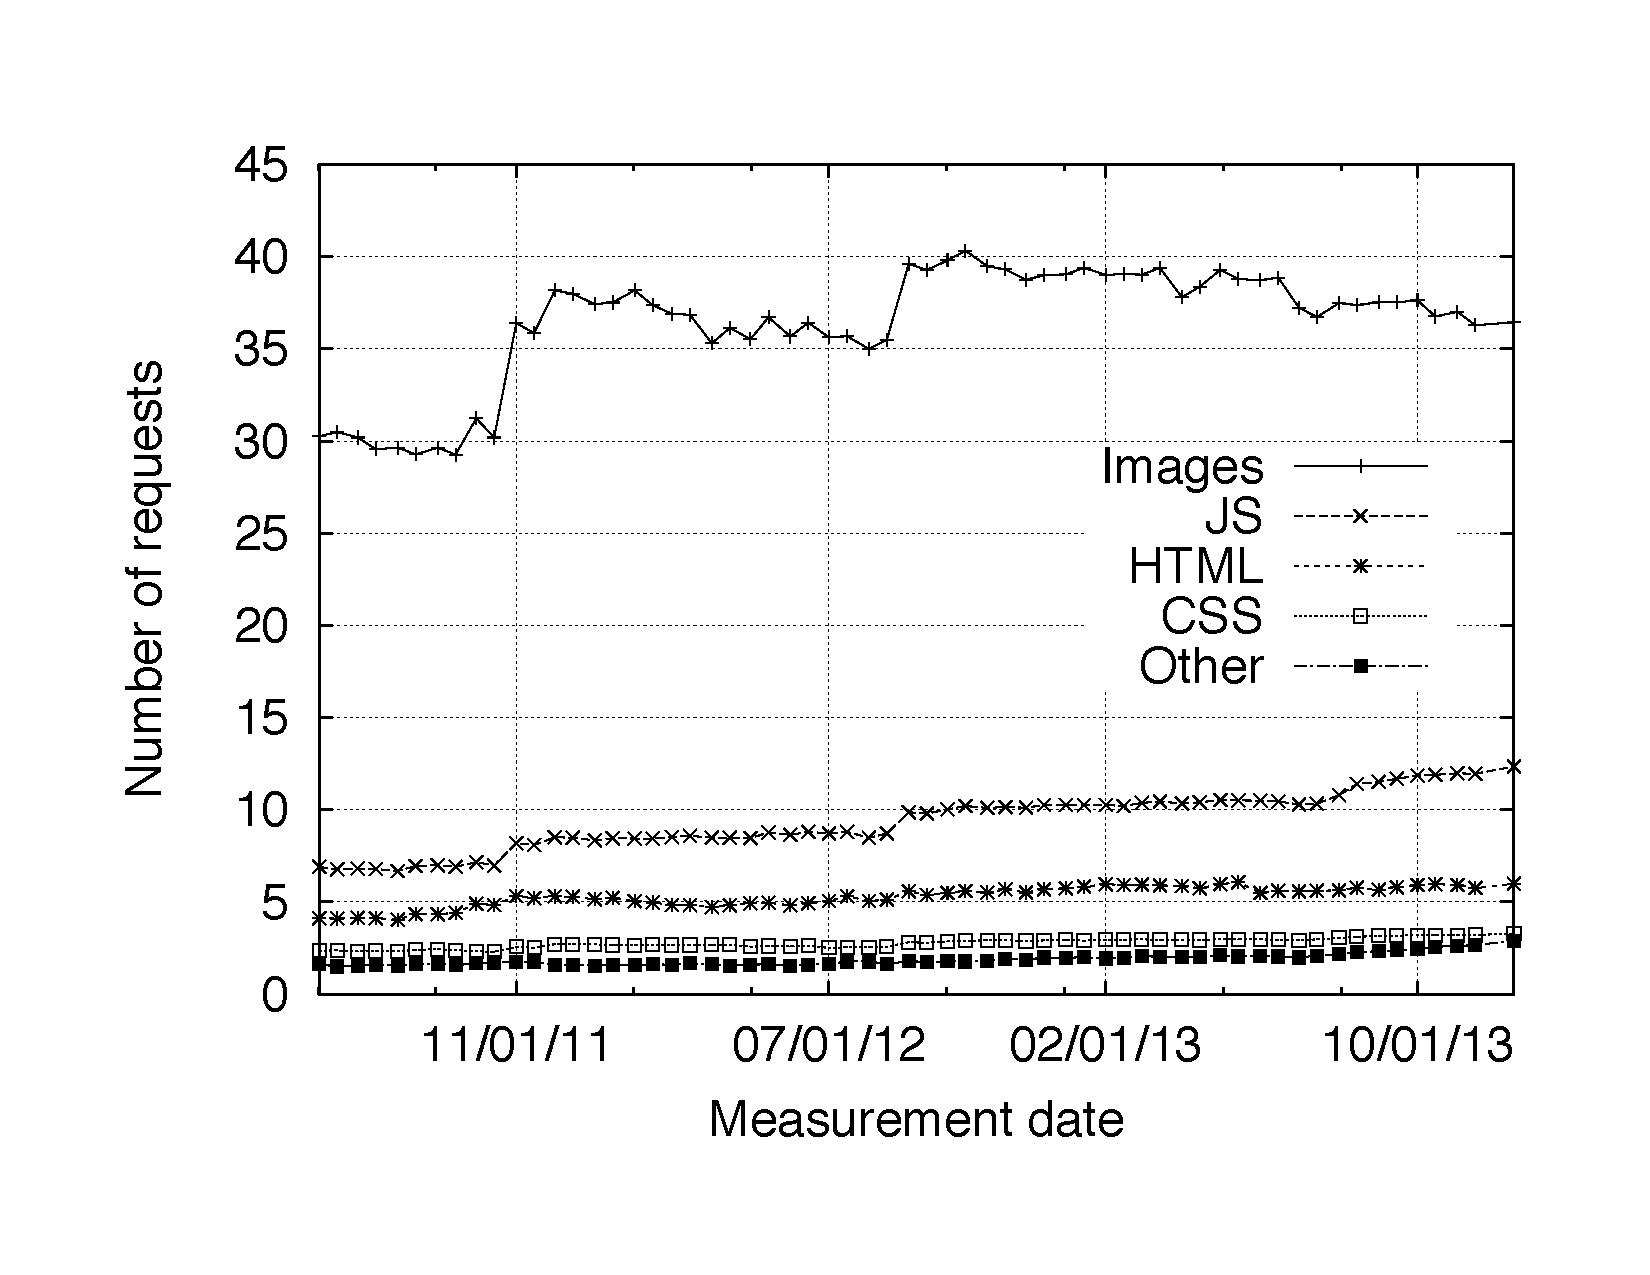
\includegraphics[width=.45\textwidth]{req_by_type_mobile_all}}\qquad
\caption{Average total number of requests for objects constituting a web page in desktop and mobile versions and decomposition into  HTML, CSS, Java Script, Images, and Other object categories.\label{fig:requests}}
\end{figure}
We initially note that the desktop versions exhibit a significantly larger number of requested objects in comparison to the mobile counterparts.
We additionally observe an overall continuous increase, which tends to have slight ``jumps'' in certain time frames (more pronounced for mobile client requests). 
These slight increases are in line with the earlier observations concerning changes to the underlying web pages constituting the measurement points in time. While significant variability between individual measurement points can be noted,  the overall trend remains steady and slowly growing.


Most notably, we witness the increase to over 100 requests on average per web page requested by a desktop client and its continued growth since the second half of 2012.
Within the same time period in 2012, the mobile web request counterpart rose to over 60 requests, with a steadily trend thereafter. 
We compare these trends for all web pages at each measurement point with the continuously present subset in Figure~\ref{fig:requests}~(a) as well.
We note that the web pages of the subset exhibit significantly lower levels of the average number of requests per web page for both versions. 
When evaluating the overall trends, however, we find that the subsets exhibit similar ones, hence corroborating our earlier observations for all pages.

Investigating the origins of the average number of web object requests in greater detail, we illustrate the composition of the average number of objects requested separated into the categories of HTML, CSS, Java Script, Images, and Other objects over time in Figure~\ref{fig:requests}~(b) for desktop client requests.
The Other category contains items such as fonts, Flash elements, as well as any remaining downloaded web page components.

We initially observe a rising trend for all categories, with the image category accounting for the most requests and the remaining ``other'' category continuing somewhat steady over time.
Keeping the overall increasing trend in mind, we note the distribution between the different categories of objects remains rather steady over time (with categories in desktop client requests accounting for approximately the following long-term averages: Images 74\%, Java Script 19\%, HTML 11\%, Others 9\% , and CSS 5\%).
For mobile requests, on the other hand, we observe in Figure~\ref{fig:requests}~(c) a nearly identical order at a lower level (with categories in mobile client requests accounting for approximately the following long-term averages: Images 80\%, Java Script 20\%, HTML 11\%, CSS 6\%, and Others 4\%).
We note that an evaluation of the categorized average number of requests per web page yields similar results for the subset of pages (omitted due to space constraints).

We conclude from these numbers that for both scenarios, the main culprit for web requests is provided by the images contained in web sites, and to a lesser extent the oft-mentioned Java Script, found in modern AJAX and HTML5 based pages in fixed as well as mobile environments.

\subsection*{Average Web Page Sizes}
\addcontentsline{toc}{subsection}{Average Web Page Sizes}
\label{ss:bytes}
We now shift our view to the average sizes of desktop and mobile client requested web pages over time as well as their most contributing factors.
We initially illustrate the total number of bytes that were required on average to download a web page to a fixed and a mobile client in Figure~\ref{fig:sizes}.
\begin{figure*}
	\centering
	\subfloat[Averages for desktop and mobile client versions.]{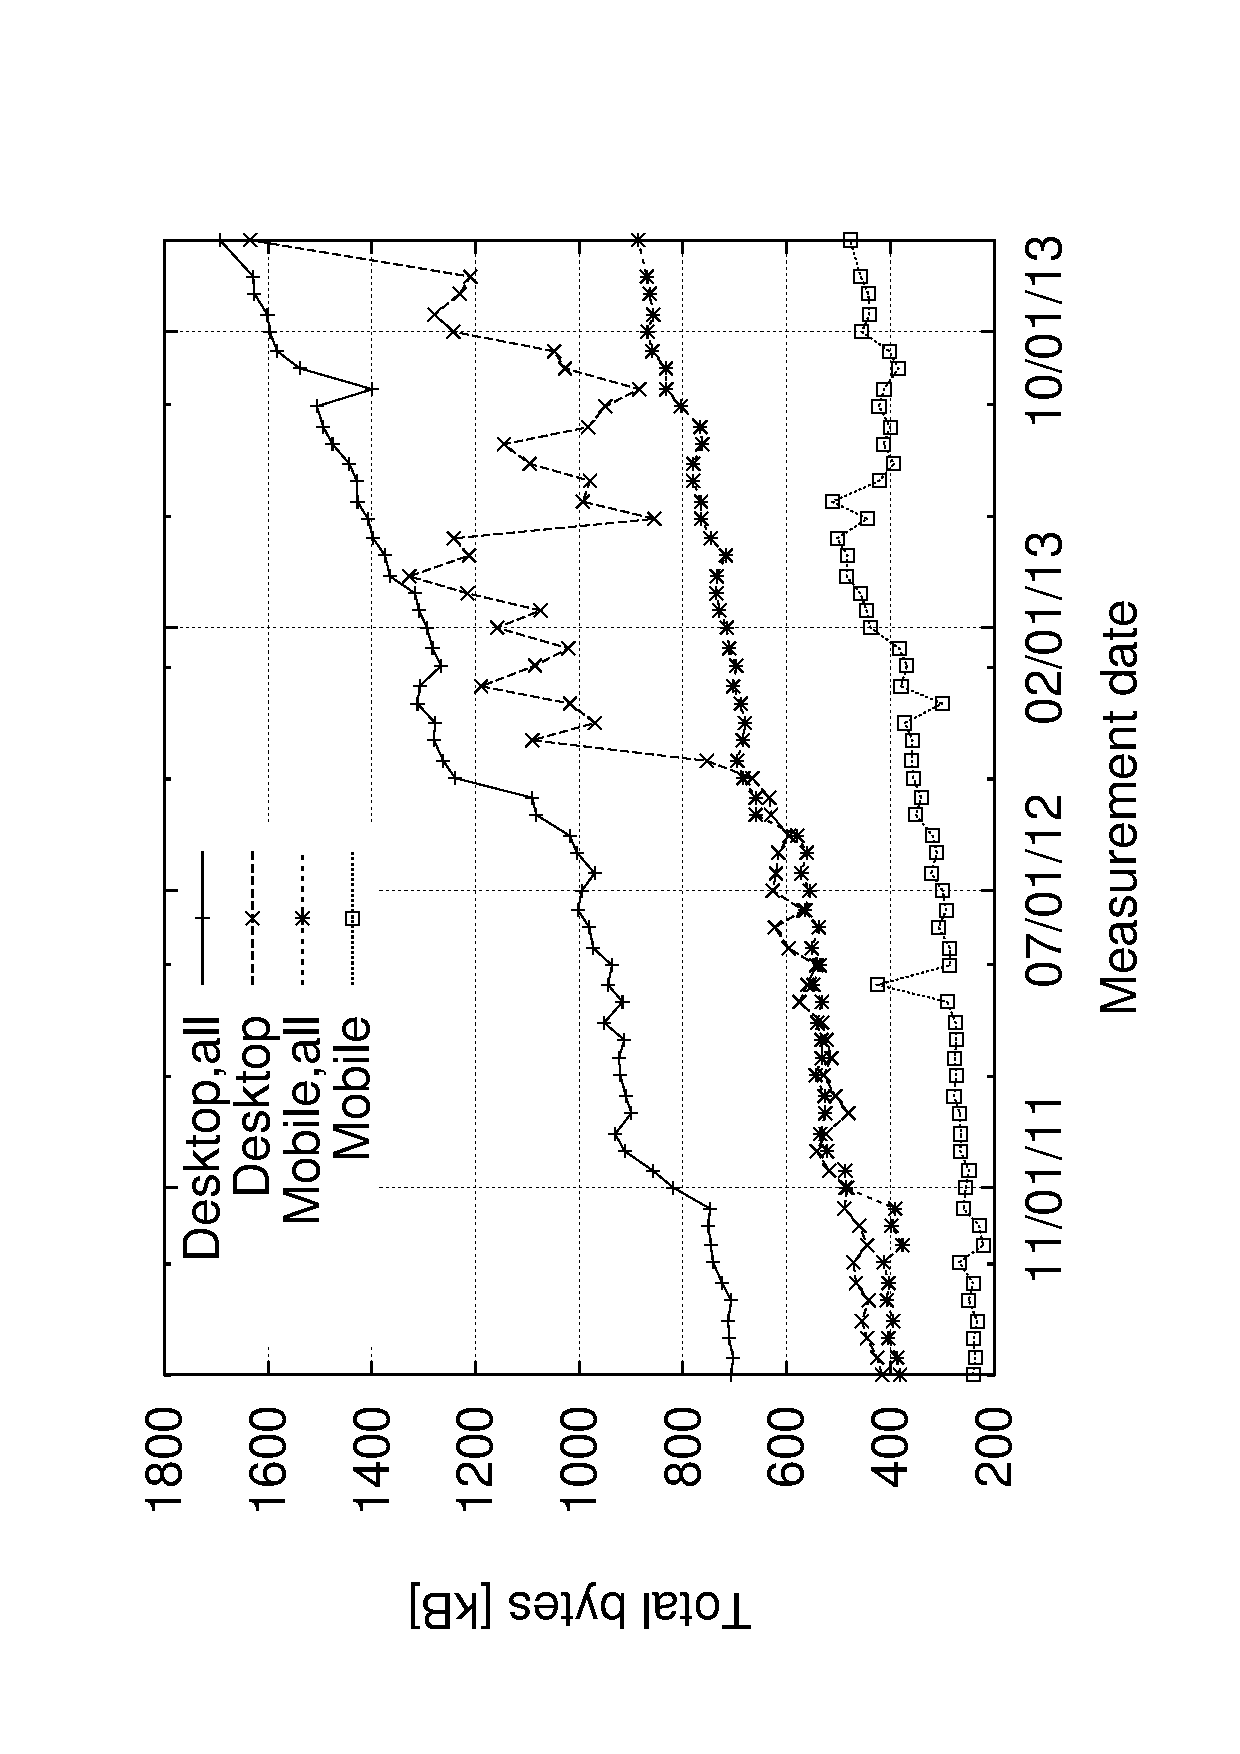
\includegraphics[width=.45\textwidth]{bytes_total_all}}\qquad
	\subfloat[Categorized for desktop client (all pages).]{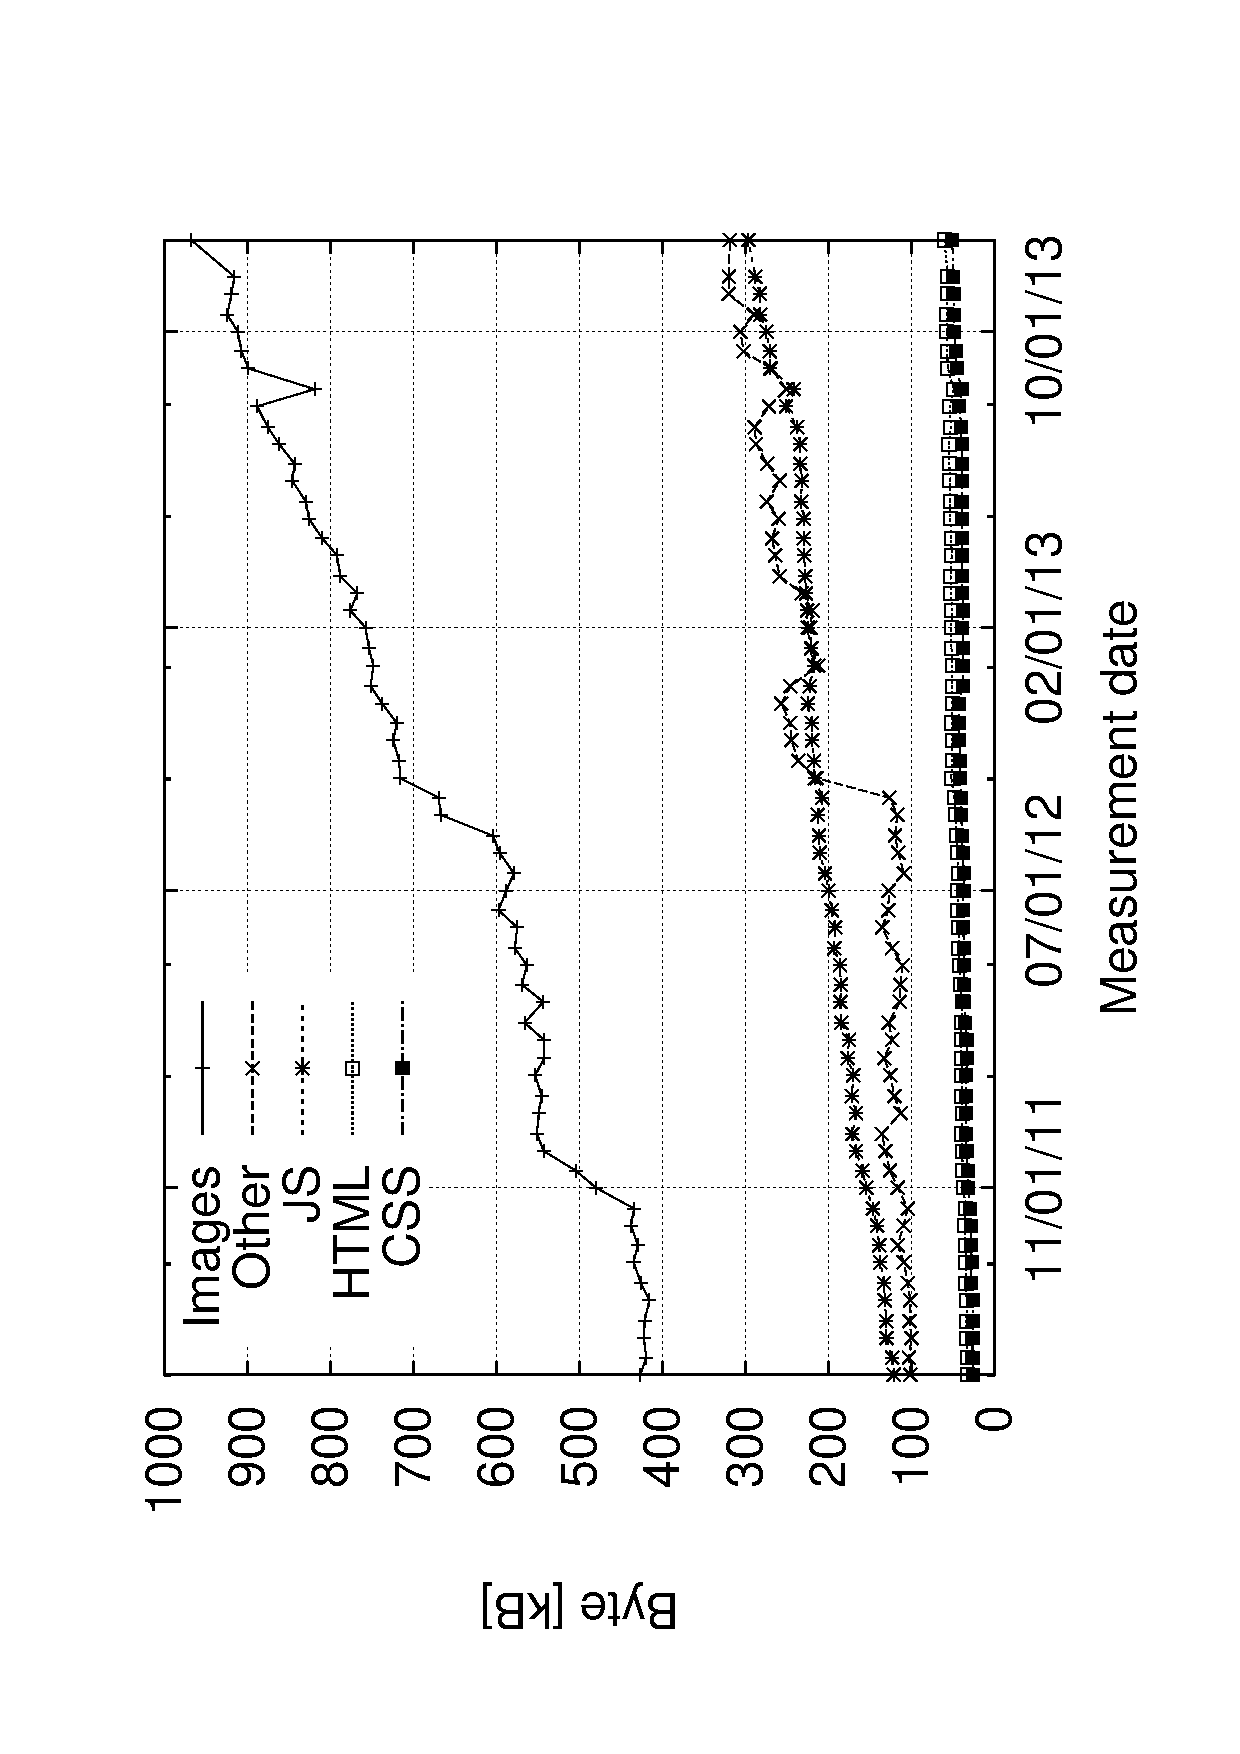
\includegraphics[width=.45\textwidth]{bytes_by_type_fixed_all}}\\
	\subfloat[Categorized for desktop client (subset).]{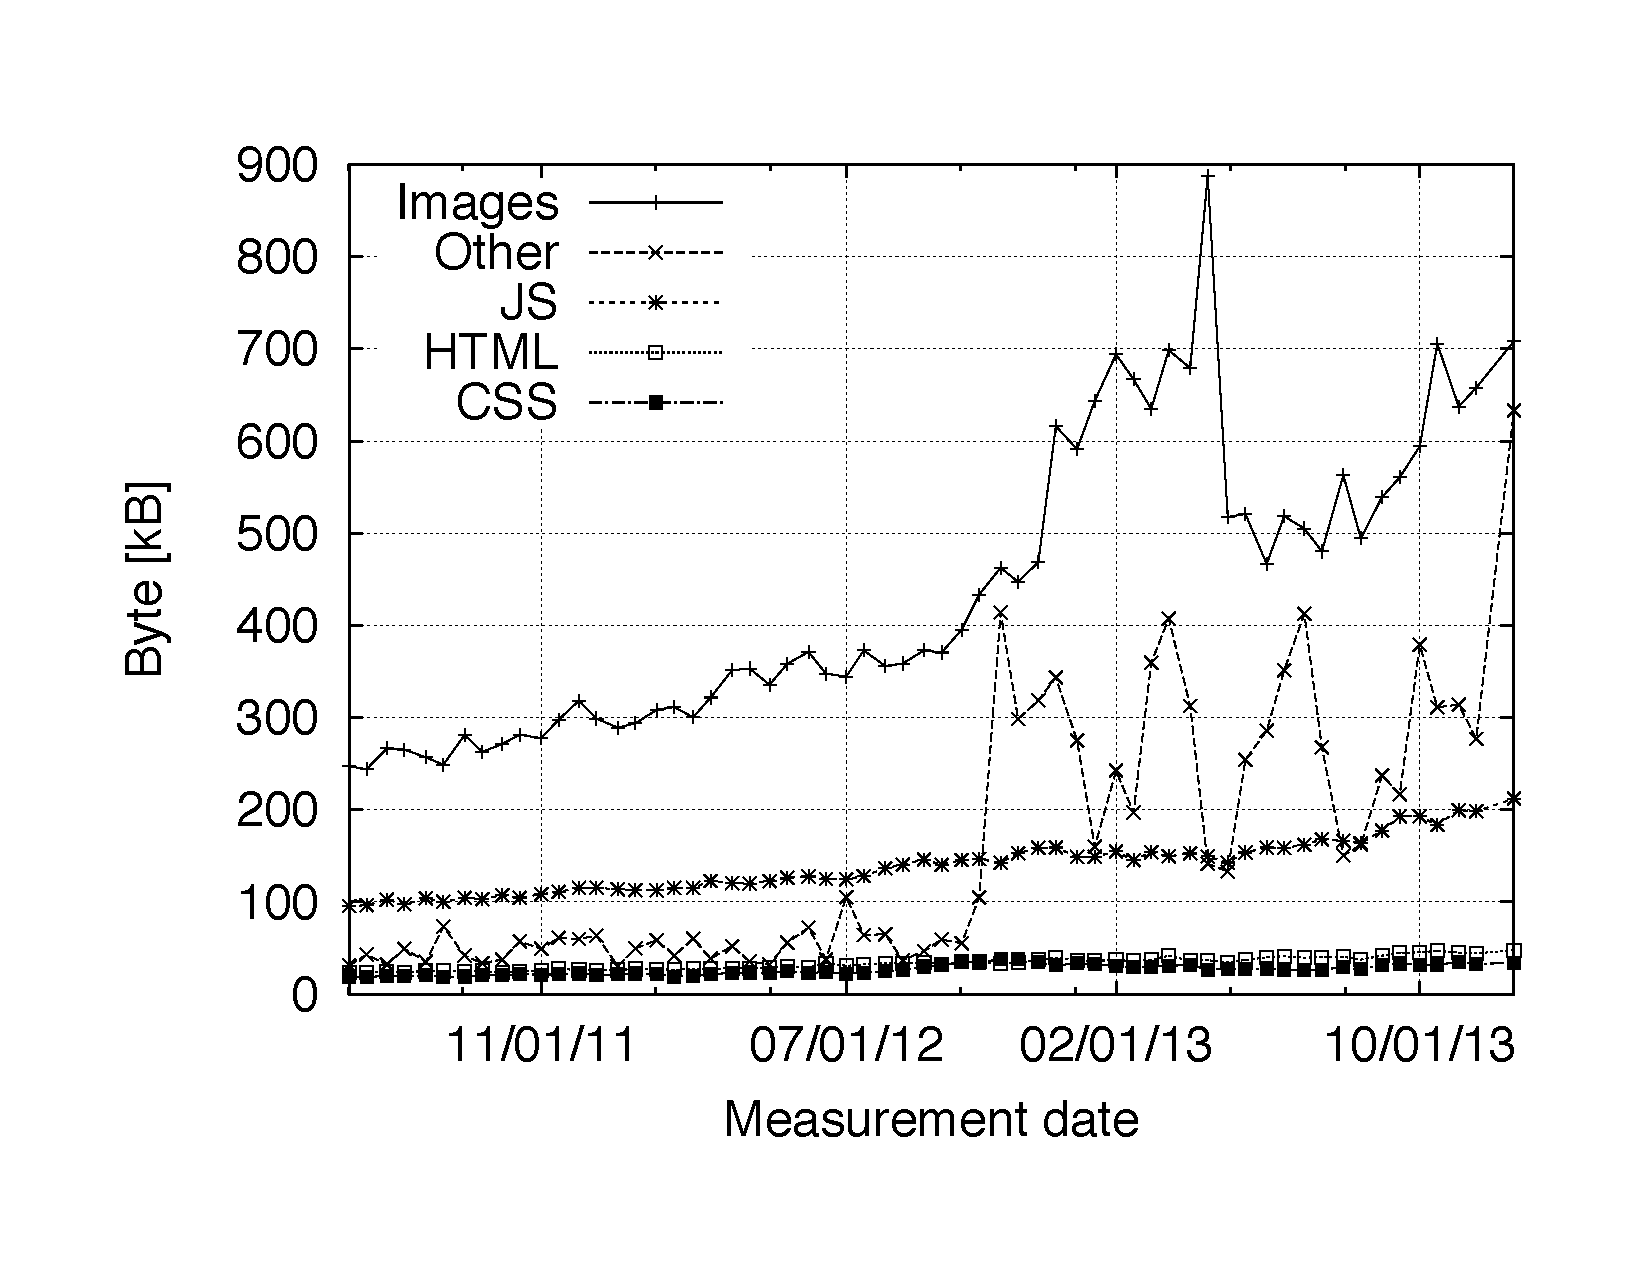
\includegraphics[width=.45\textwidth]{bytes_by_type_fixed}}\qquad
	\subfloat[Categorized by category for mobile client (all pages).]{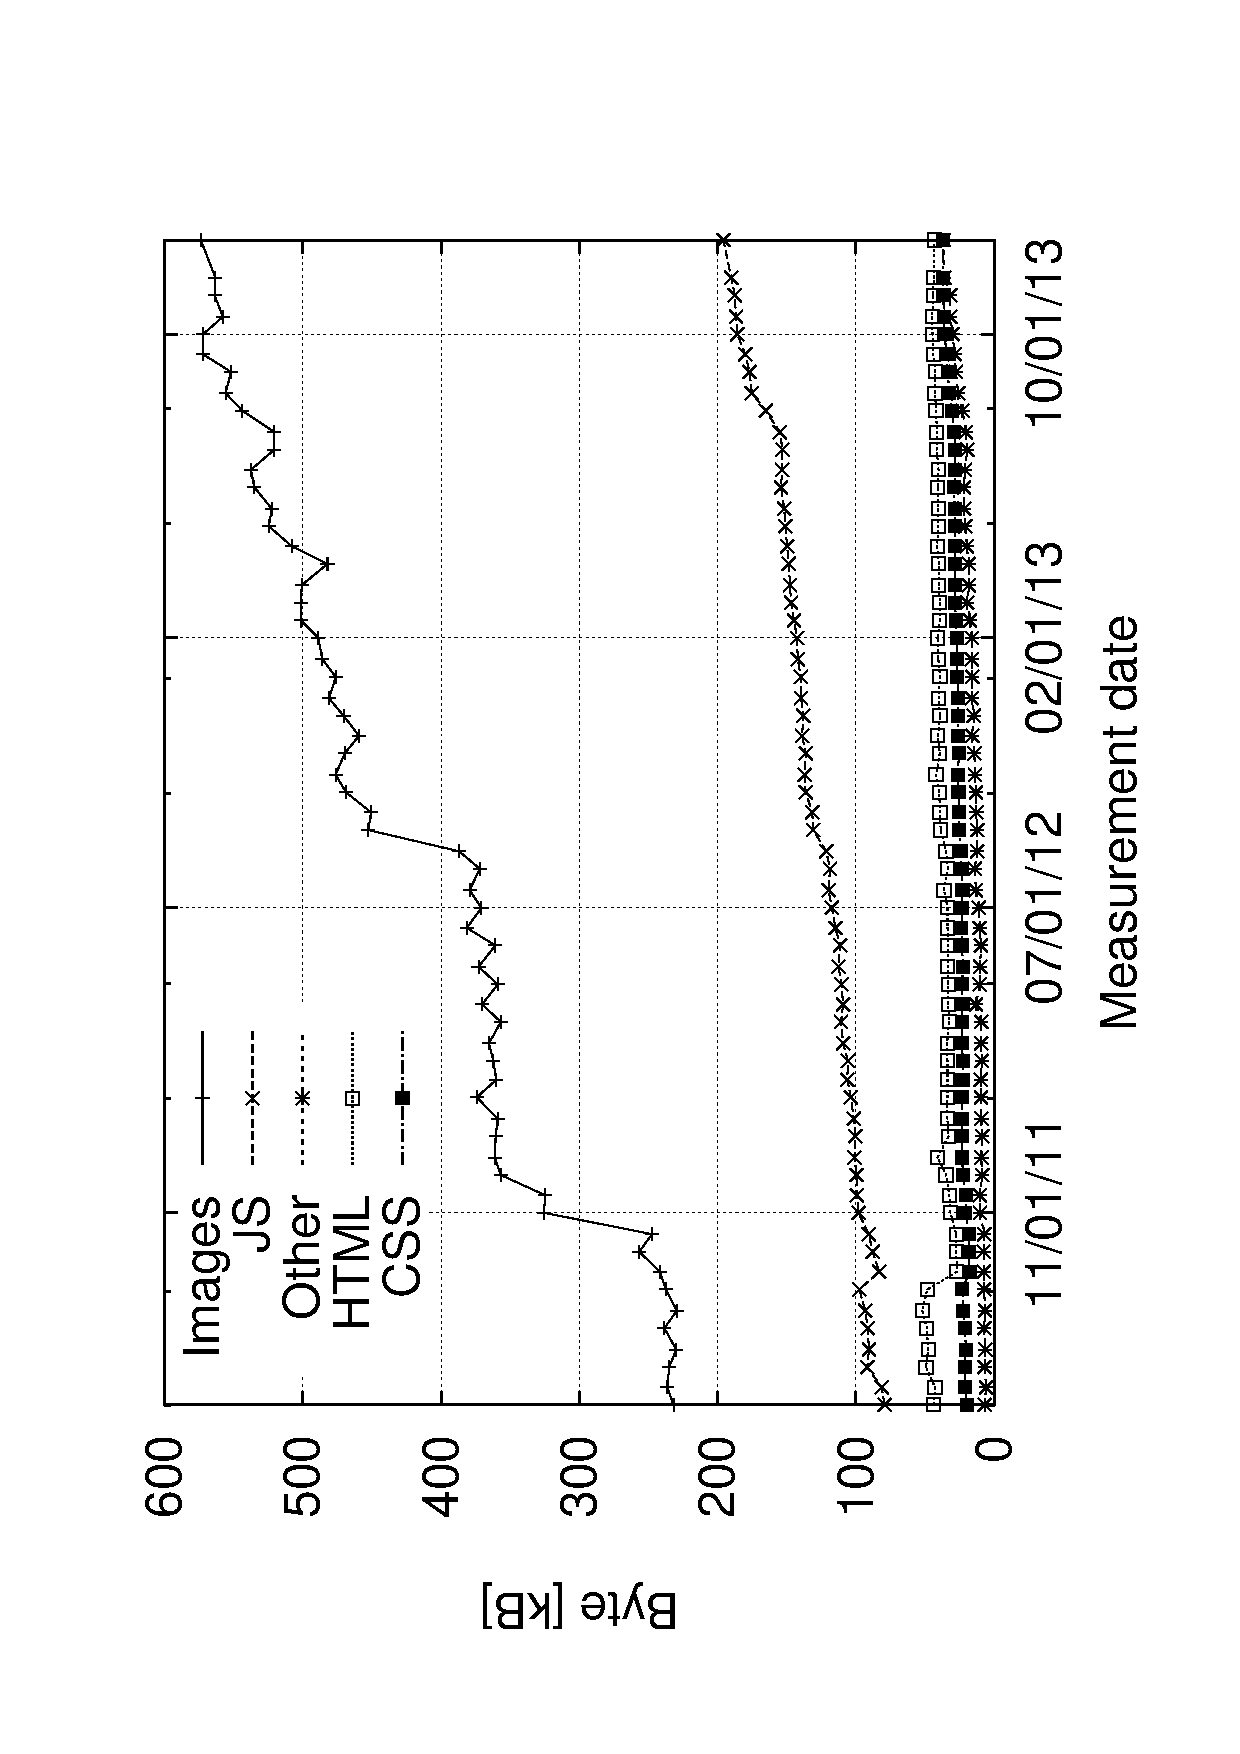
\includegraphics[width=.45\textwidth]{bytes_by_type_mobile_all}}\qquad
	\caption{Average total number of bytes constituting a web page in desktop and mobile versions and decomposition into  HTML, CSS, Java Script, Images, and Other object categories.\label{fig:sizes}}
\end{figure*}

We observe that the fixed sizes are always larger than their mobile counterparts and that both continuously increase over time. 
This leads to the average web page size to have increased from 0.71 MB in June 2011 to over 1.5 MB in December 2013 for desktop client and from 0.38 MB to almost 0.9 MB for the mobile counterparts in the same time frame.
In greater detail, we note that the average increase in average web page sizes over time for fixed web pages during the evaluated time period is around 3\% per month or approximately 41\% per year, while the mobile counterparts feature an increase of 3\% or 40\%, respectively.
We also find that the average mobile web page sizes currently trail their desktop counterparts by approximately 1.75 years, which likely will increase due to the difference in average growth rates (1.57\% vs. 1.47\% on average in every two week time period for fixed and mobile web pages, respectively).
Similar to the average number of requests, we compare the subset of 46 web pages to the complete dataset in Figure~\ref{fig:sizes} as well.
We observe a similar behavior here with the subset's reduced average number of bytes for the first half of the observation period. In the second half, the fixed web pages exhibit a significant increase in the average sizes and variabilities thereof. 
However, the overall rising trend is present for both versions and corroborates our overall rising trend observations.

Investigating the origins of the average number of web page sizes, we illustrate the composition of the average number of bytes requested separated into HTML, CSS, Java Script, Images, and Other object categories over time in Figure~\ref{fig:sizes}~(b) for desktop client requests.
We immediately note that while all components are increasing in size over time, the main contributors to the growth are the Images and Other web page object categories.
More specifically, we note that the three main contributors to total web page sizes are images, other components, and Java Script. 
While the number of bytes contributed by Java Script has slowed in growth, images (which have almost doubled in the number of bytes) and other web page items (which more than doubled) continue their growth over time.
We can attribute this behavior to the richer web experience that users demand, with additional interactivity and visually stimulating appearance.
HTML and CSS components of web pages, on the other hand contribute only a minimum amount of data, with little increase over time.
Comparing the detailed categorized values with the subset of web pages in their desktop versions, we note that the origin of the radical increase in average sizes can be attributed to the increase of data in the images and other categories.
Some of these individual spikes can be attributed to individual outliers, such as a handful of web pages exhibiting very large object sizes. On http://www.tumblr.com on April 15, 2013, an approximate 15 MB image was encountered, which can be seen as anecdotal representation of automated processes (such as the background image for that particular homepage being picked from user posts) lacking optimization routines (such as downscaling in this case).


Shifting the view to the average sizes of the web page components for mobile clients, we also note an overall growth trend for all categories as illustrated in Figure~\ref{fig:sizes}~(d).
For mobile clients, however, the overall average web page sizes stem mainly from images and secondly Java Script. 
The remaining three categories contribute significantly less data and exhibit a slower growth.
It is interesting to note from comparison with the desktop counterparts, that the average mobile client image sizes are approximately two thirds of their desktop counterparts.
Unlike the average number of requests, however, the average number of bytes clearly identifies Java Script for mobile devices as one of the main causes of increased web page sizes. 
We exclude the detailed evaluation of the subset's characteristics here, as the results resemble earlier observations and their conclusions.


\subsection*{Data per Web Page Object}
\addcontentsline{toc}{subsection}{Data per Web Page Object}
Combining the two former evaluations, we now evaluate the average web page object request size.
We illustrate the overall and categorized views in Figure~\ref{fig:relative}.
\begin{figure}[]
	\centering
	\subfloat[Averages for desktop and mobile client versions.]{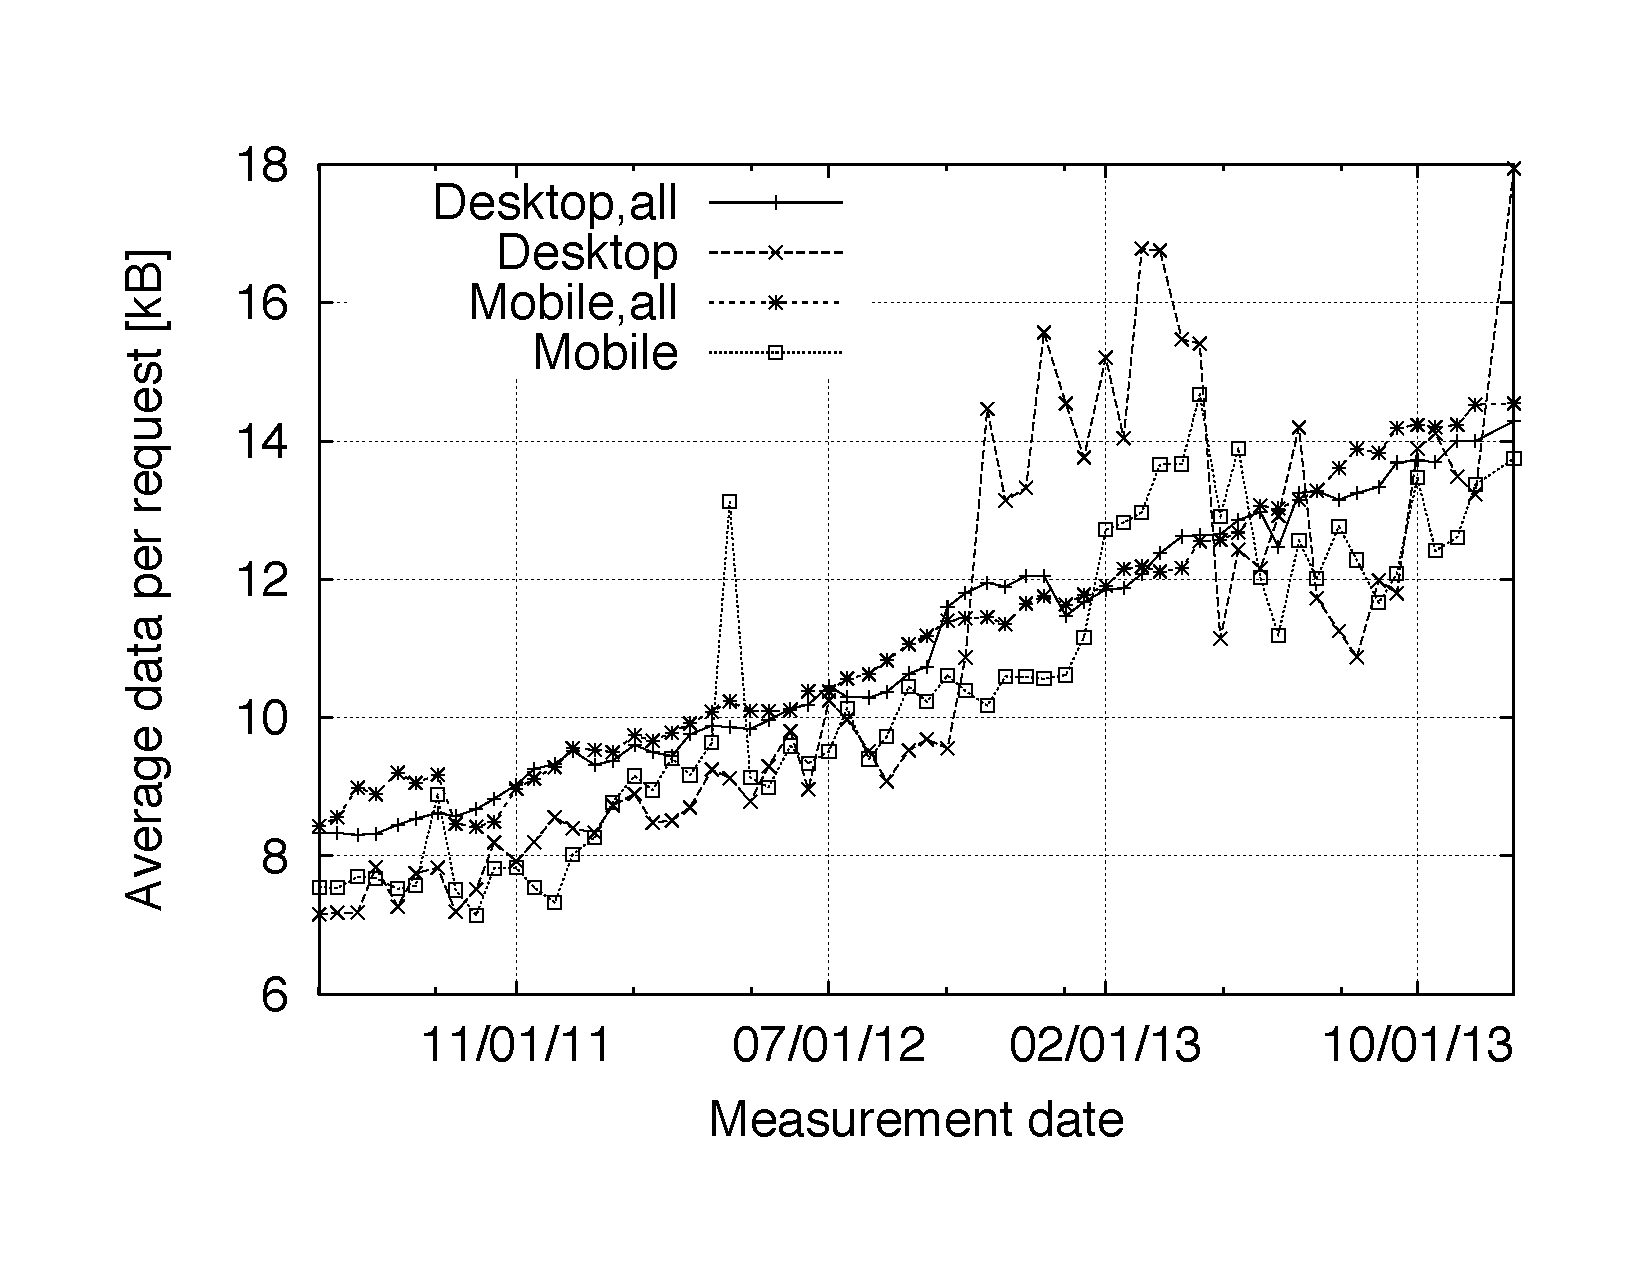
\includegraphics[width=.45\textwidth]{bpr_all}}\\
	\subfloat[Categorized for desktop client (all pages).]{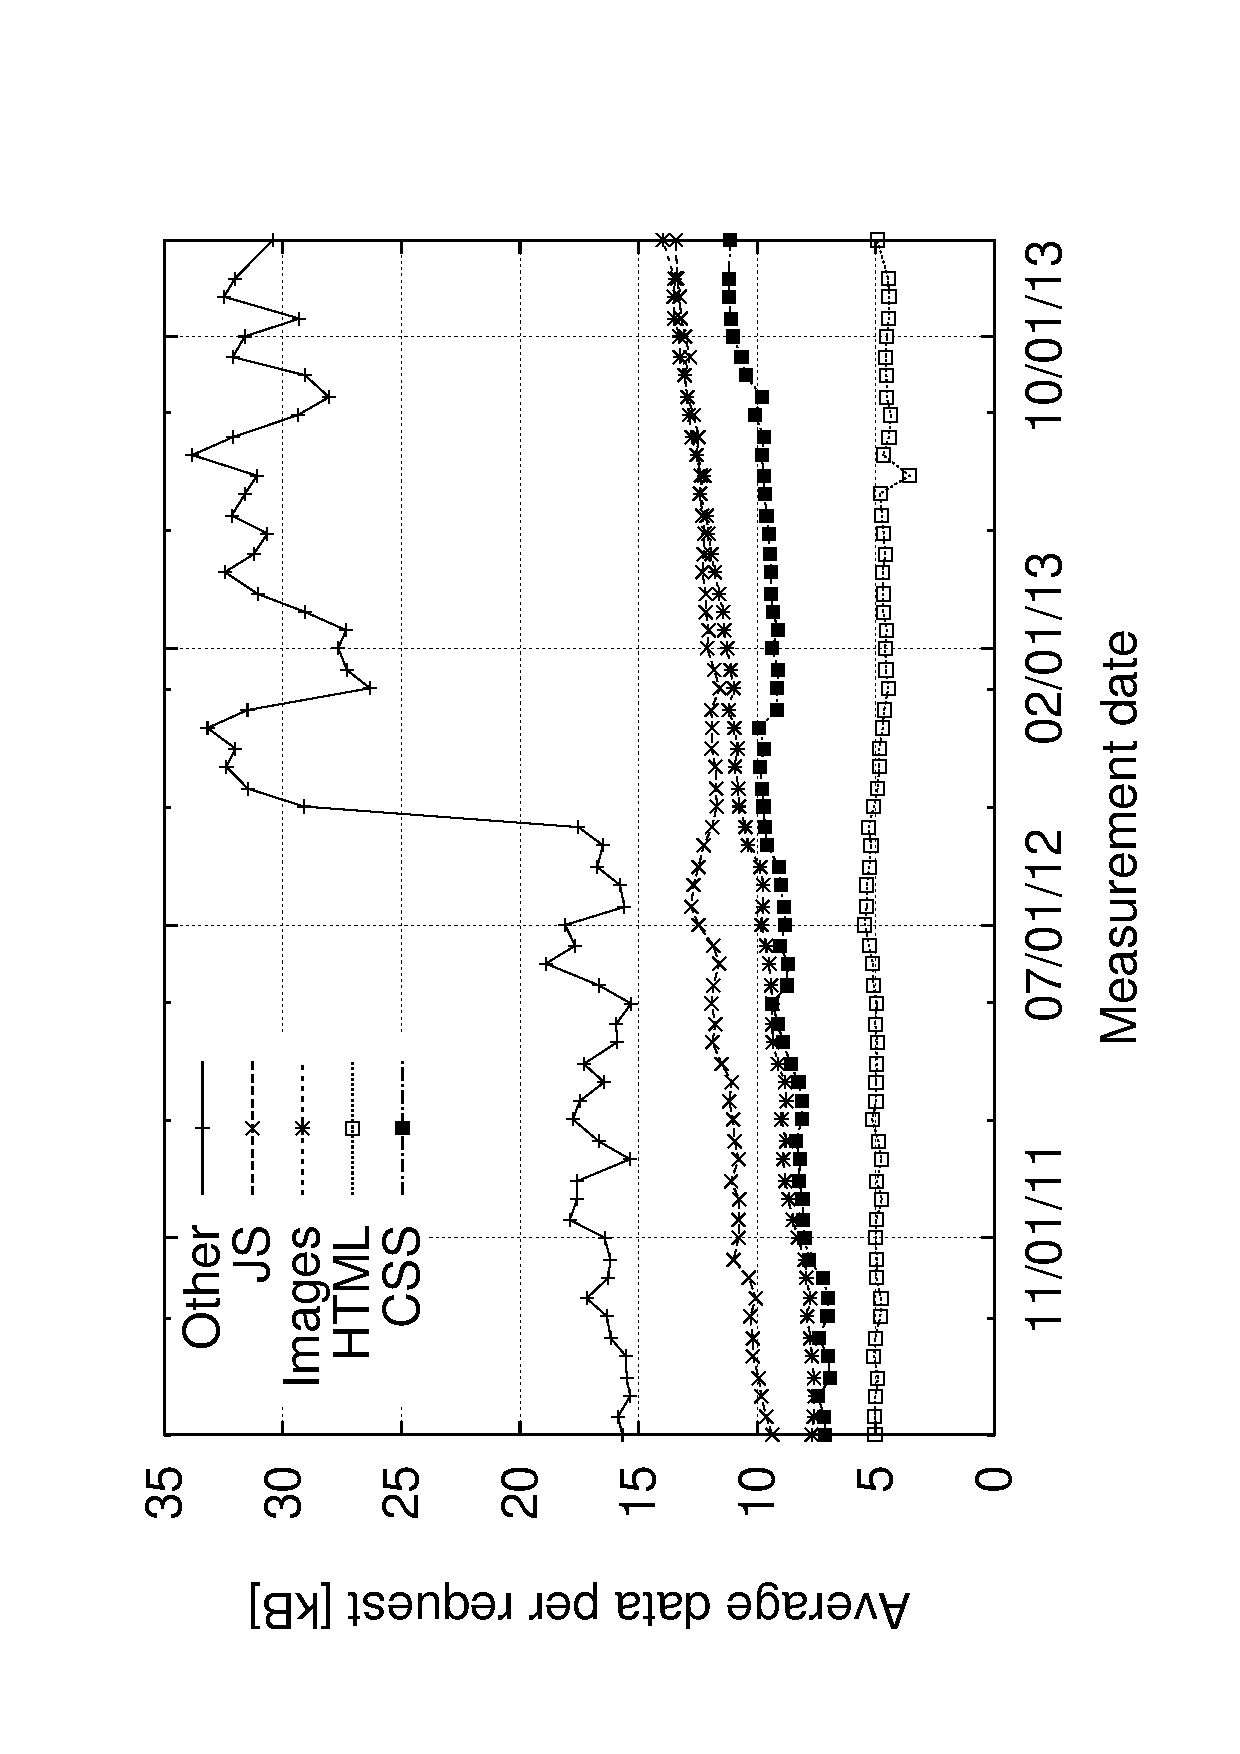
\includegraphics[width=.45\textwidth]{bpr_by_type_fixed_all}}\qquad
	\subfloat[Categorized for  mobile client (all pages).]{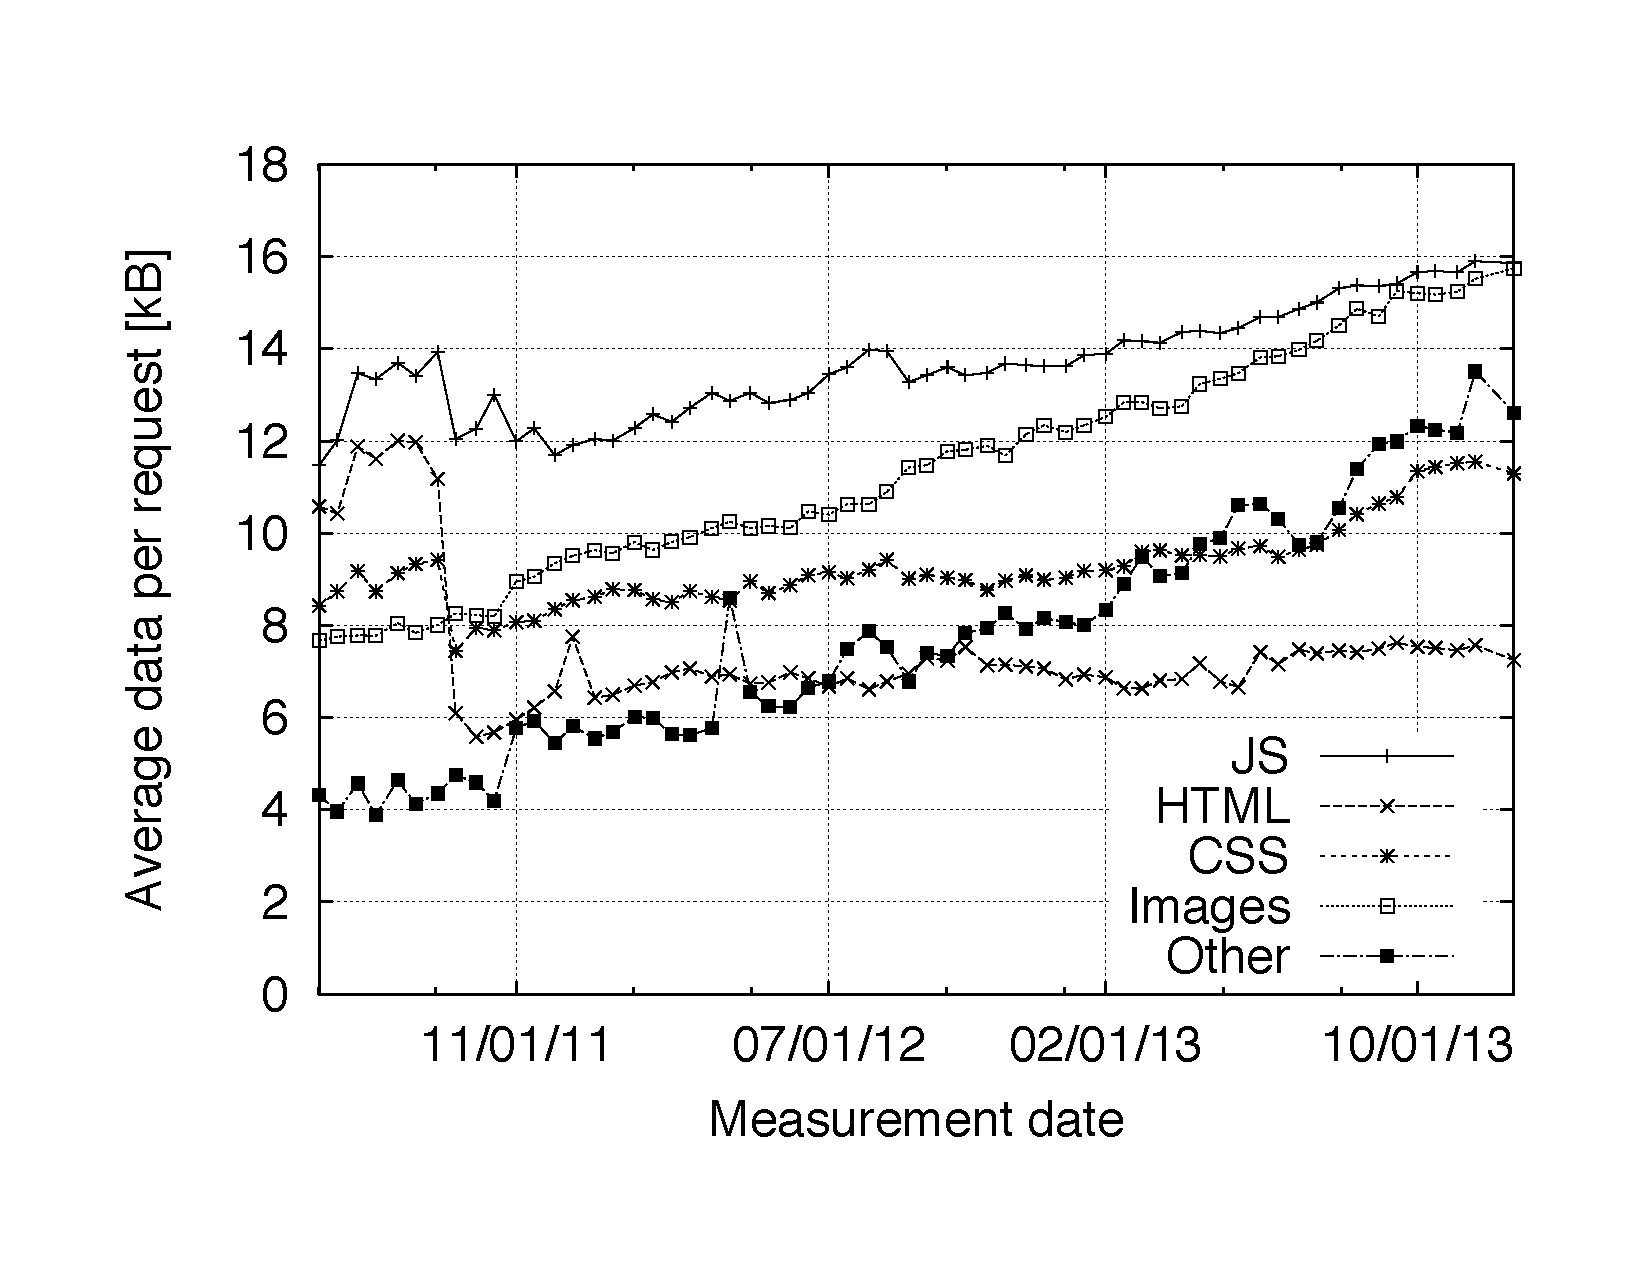
\includegraphics[width=.45\textwidth]{bpr_by_type_mobile_all}}
	\caption{Average number of bytes per web page object request for desktop and mobile versions and decomposition into  HTML, CSS, Java Script, Images, and Other object categories.\label{fig:relative}}
\end{figure}
For the average number of bytes per web page request, illustrated in Figure~\ref{fig:relative}~(a), we note a steady increase for both desktop and mobile client requests. 
In greater detail, we note that the overall trend for both request origins is rather linear and close.
In turn, we note that both feature an almost identical overall growth rate of about 0.9\% every two weeks.
Verifying these original findings by comparing them with the smaller size subset of web pages, we note that even these pages exhibit the same underlying trend, albeit in conjunction with increased variability.
This is a finding with great long-term implications for simplified approaches to modeling, e.g, in capacity determination scenarios.

Next, we investigate the behavior more closely by evaluating the HTML, CSS, Java Script, Images, and Other categories separately for the desktop and mobile clients in Figures~\ref{fig:relative}~(b) and \ref{fig:relative}~(c), respectively.
For desktop requests, we note that the highest number of bytes per request can be observed for the Other category, with a pronounced ``jump'' in the time frame of base URL adjustments in the underlying dataset. 
In turn, we reason that more components, such as Flash or font data, are included in the larger underlying set of web pages evaluated, which results in the current level of around 33 kB per request in this category.
For Java Script and CSS data per request, we observe  initially growing trends, which have slowed over time and now are moving beyond 14 and 11 kB, respectively.
Images, on the other hand, continue their growing trend and now feature about 14 kB per request.
The actual HTML markup request size has remained relatively constant at around 5 kB.
For requests from mobile clients, on the other hand, we note that the largest amount per request is observed for Java Script, with currently growing sizes above 15 kB.
The Images and Other categories also feature a significant growth for mobile client requests, which have risen above 15 and 12 kB, respectively.
The HTML and CSS categories are fairly stable with only minimal growth over time, which is similar to the trends observed for the desktop clients.

In comparison, we note that while both average client request sizes are comparable with respect to their level and growth rates, the actual composition is significantly different. 
While desktop request sizes are mainly determined by the Other category data, such as Flash or fonts, and increasingly images, mobile requests are mainly characterized by Java Script and Images.
The reason behind this behavior could be the increased level of rich media inclusion for desktop clients (e.g., using Flash), whereas automatic adjustments performed (e.g., using Java Script) disable this for mobile clients, where this is not desired. 
Furthermore, we note that the average amount of bytes per image is fairly close (even a bit higher for mobile), which could be due to increased utilization of content management systems.
These commonly utilized frameworks typically adjust web page layouts and theming elements based on the requesting client, e.g., format for mobile display sizes and utilize smaller sized theming elements. The actual main content elements, however, typically remain unchanged (which, in turn, results in identical downloads of the larger sized content images).

\subsection*{Caching of Web Page Objects}
\addcontentsline{toc}{subsection}{Caching of Web Page Objects}
One of the main assumptions for the prior evaluation was that the data represents ``first views,'' i.e., the dataset's underlying measurements do not consider the caching of web pages after initial visits. 
The individual entries in the datasets obtained from httparchive.org, however, additionally contain the max-age header (amongst other, such as expiration) directives for evaluation of the maximum lifetime of objects on the requesting device. The locally cached data can have a positive impact on the required network access, especially for mobile devices.
We illustrate the different max-age values obtained from the data in Figure~\ref{fig:maxage}~(a) for desktop client requests.
\begin{figure}
	\centering
	\subfloat[Desktop clients]{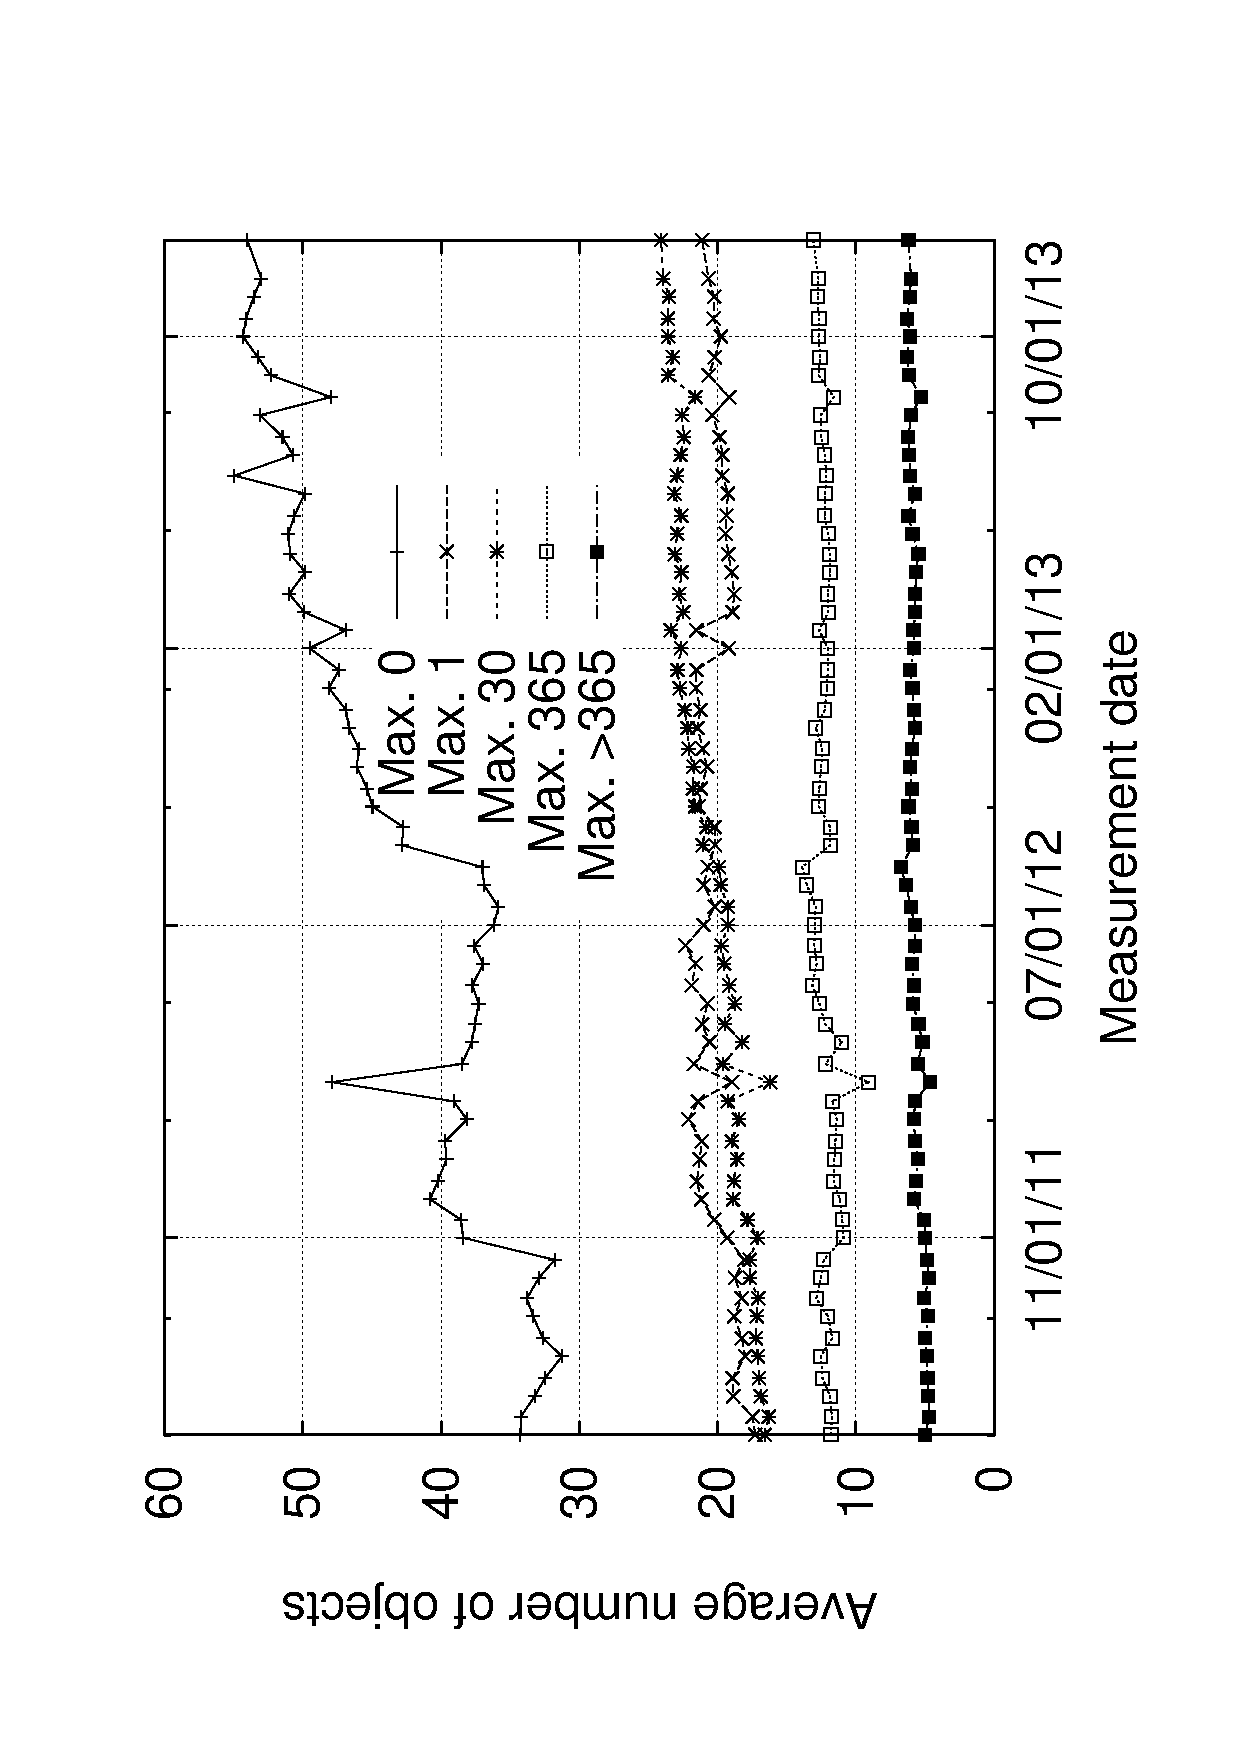
\includegraphics[width=.45\textwidth]{cache_fix_all}}\qquad
	\subfloat[Mobile clients]{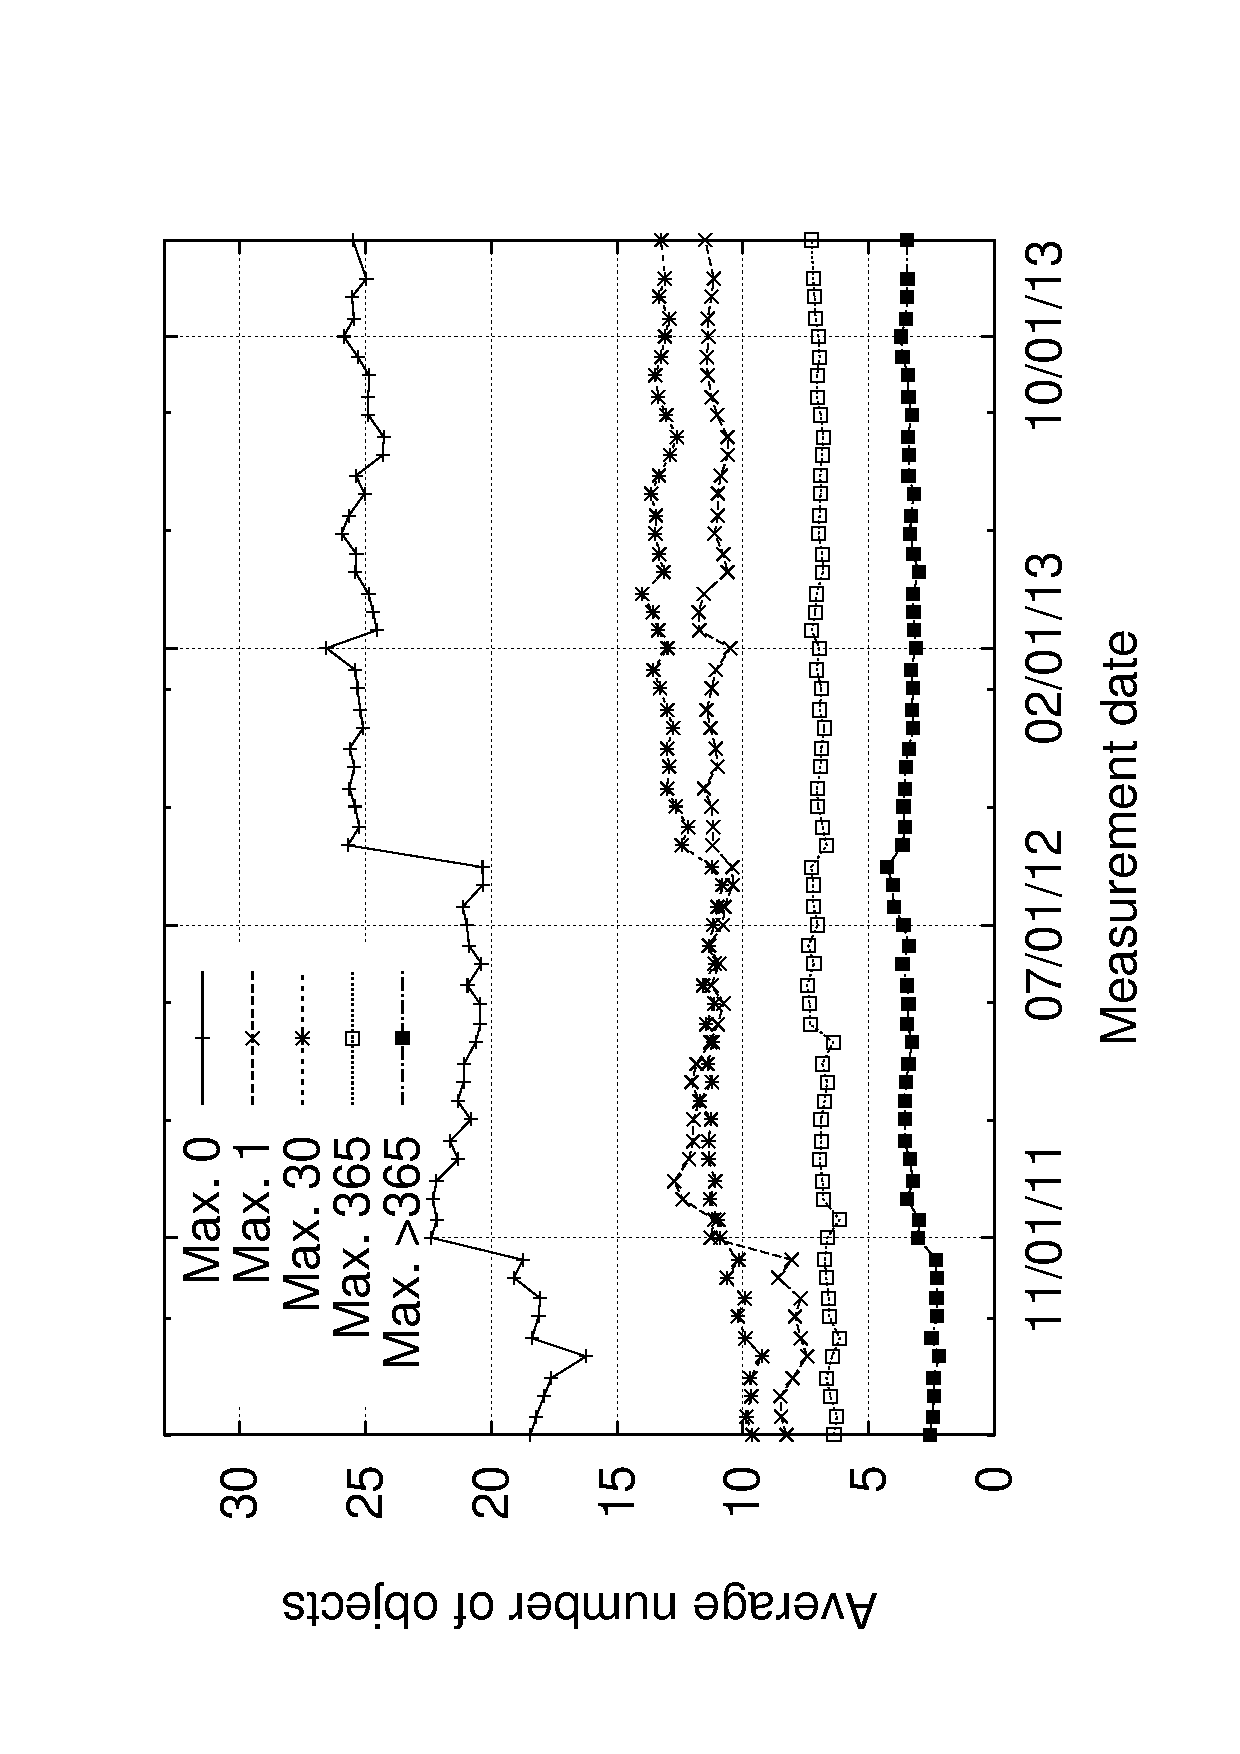
\includegraphics[width=.45\textwidth]{cache_mob_all}}\\
	\caption{Maximum age of web page objects for desktop and mobile web clients.\label{fig:maxage}}
\end{figure}
We observe that the largest fraction of items cannot be cached beyond a day, and in turn requires frequent downloads if web pages are visited infrequently. 
More importantly, this is the only category that exhibits significant continued growth.
Over the time horizon we consider here, items that are stored between one and up to 30 days can be considered regularly downloaded at a comparable level, while only a relatively small number of objects can be considered invariant due to larger maximum allowable cache ages.
For the mobile client counterparts illustrated in Figure~\ref{fig:maxage}~(b), we initially note a similar level and continued growth for the average number of objects that are able to be cached below a day (considering the overall average number of objects requested as discussed in Section~\ref{ss:objects}).
Objects that require regular, but less frequent downloads as well as more invariant items follow the trends observed for the desktop client.
Overall, the implication for mobile clients is that the fraction of requests with a shorter cache lifetime constitutes the majority of requests and in turn will require frequent downloads if web pages are visited infrequently.


\section*{Implications}
\addcontentsline{toc}{section}{Implications}
\label{s:discuss}
One initial limitation of our dataset is the evaluation of landing pages only, which, however, could be seen as an actual upper limit, according to \cite{BuMaSe13}. 
Overall, we find significantly growing trends for the average web page number of objects and their sizes.
The immediate implications from the growing trend of the number of web request per fixed and mobile website versions and their respective size is that the pressure on access networks capacity growths will continue, see, e.g., \cite{Ci13} for a detailed separation into typical business and consumer categories of accesses Internet data.
We find significant similarities between the desktop and the mobile versions of the popular web pages that were part of this evaluation. 
Mobile counterparts of desktop page versions typically feature less objects and smaller sizes; both characteristics typically also exhibit a significantly slower growth.
As briefly outlined by the authors of \cite{BuMaSe13}, the reduced number of servers and number of objects involved likely can be seen as an indicator of the correlation between the two different versions of popular web pages.

As previously outlined in~\cite{ThAgNiBoSi12}, Java Script objects in mobile web pages are a main contributor to the rendering power consumption, and we find significant amounts of Java Scripts to be contained in average web pages.
More importantly, we conceive that there is a significant amount of data and requests in average mobile pages that is dedicated to image and other objects, which will contribute significantly to the combined transmission and rendering energy costs, as outlined in \cite{ThAgNiBoSi12} as well.
Optimization efforts that target mobile clients specifically should in turn focus on these categories of data, specifically while taking more advantage of caching possibilities, as the transmission energy contributes a significant amount to the total energy required.
%
% Correlation
%
Combining the two prior evaluation categories, the average total number of bytes per request for desktop and mobile web pages are very similar and exhibit a linearly growing trend.
This finding for the larger dataset is additionally corroborated by evaluation of the continuously present web pages, which exhibit the same trend, albeit at higher levels of variability.
While some of the greater details highlight smaller differences by respective type of object requested, the overall direct correlation between the two gives rise to future research questions.
%
% Comparison
%
Comparing our results with prior longitudinal studies in \cite{CaAlPa10,IhPa11}, we note several interesting similarities and other findings, within the constraints given by each of the three studies.
First, both prior studies cover date ranges prior to our study's time frame, ending in 2009 and 2010, respectively. They are based on actual user request analyses derived from proxy monitoring, whereas our study specifically utilizes an evaluation of the landing pages of popular web sites, which can be regarded as more static.
The HTTP GET transaction size evaluation performed in \cite{CaAlPa10}, which is also corroborated by the median page size growth ending around 133 kB reported in \cite{IhPa11}, provides an almost seamless trend continuation over time (especially when considering the different study parameters, which include follow-up session browsing).

As indicated by \cite{IhPa11} for prior years, our study also finds a significant shift in the bytes per object -- with  images constituting the majority of traffic in both request scenarios.
In the recent years we evaluate, however, we now note a shift to the desktop client's Other category, while mobile clients exhibit a significantly smaller overall size and lower amounts of data in the Other category.
Comparing initial caching observations here with the results provided in  \cite{CaAlPa10,IhPa11}, we note that the overall number of cacheable objects is increasing for the desktop requests, which is in line with the GET request savings described in \cite{CaAlPa10}, where about 20-25\% were identified.
Similarly, \cite{IhPa11} reports 27-37.1 \% of objects to fall into this category for US-based traffic, resulting in byte savings of 16.8-28.1\%.
In turn,  the cache-based object retrieval can reduce the waiting times to amounts that fall within positive user experience time frames, see, e.g., \cite{NiUeNa10}.
In conclusion, our study finds a continuation of prior longitudinal studies when overall trends are regarded, but differences in the lower-level shifts of requests and data by categories and requesting device.

\section*{Conclusion}
\addcontentsline{toc}{section}{Conclusion}
\label{s:conc}
This overview represents the first longitudinal and comparative study of the current state and changes of the World Wide Web, as seen by current fixed and mobile clients when requesting web pages.
We utilized the publicly available data from httparchive.org, an industry-supported web page statistics archival project, to outline major trends and resulting implications.
For the number of web-page requests, we noted an overall growing trend, with a slightly higher rate for desktop versions of web pages, continuing trends observed in the past. 
Modern web desktop page versions feature well above 100 object requests on first views, while mobile versions trail above 60.
Similarly, we noted a rapidly increasing trend with regard to the average web page sizes, with desktop pages surpassing 1.5 MB in initial view size, while mobile pages trail at more than 50\%.
Most astonishingly, this study found that the average bytes per request are within close proximity for fixed and mobile clients and exhibit both comparable as well as significant growth rates.
When performing decomposition into categories, we found that Image, Other (such as Flash or fonts), and Java Script objects are the main contributors to web page sizes for both clients. Furthermore, the most requests for objects on first view are attained for the Image category of web page objects, again independent of the client type.
We also evaluated the potential of caching objects for subsequent views of web pages, whereby we found that most web page objects exhibit very short cache life times of a one day maximum.
Our overview thus suggests that there are significant opportunities for future research and optimization efforts for efficient mobile web content delivery. 
Specifically, our findings indicate the need for more optimization and client considerations when designing modern web pages and frameworks that are utilized for their delivery.







NEED TO UPDATE THIS SECTION AS PAPER WAS UPDATE ON 2/9 WITH CONTENTS OF USER SESSION MODELING SIMULATION



\chapter{Modeling Landing Page Characteristics for
Mobile Web Access Performance Evaluations on
Object and Page Levels}

\section*{Introduction}
\addcontentsline{toc}{section}{Introduction}
Smart mobile devices with ubiquitous connectivity have become popular worldwide and their utilization has increased the amount of traffic in wireless networks tremendously. 
As mobile users employ their always--present devices to access web--based services, additional forecasts include a shift of the main access of the world wide web from fixed desktops to mobile clients. 
Cisco, Inc. predicts that this current trend will result in a steady growth of mobile data for years to come~\cite{VNI14}.
As the primary means of web access changes, evaluations employing desktop client web access strategies not necessarily reflect the potential for optimizations.
While on the network provider side, caching can readily yield savings through caching~\cite{IhPa11}, the mobile client side becomes increasingly significant due to mobile devices typically exhibiting limitations with respect to battery capacities.
The composition of web pages, e.g., has an impact on battery consumption~\cite{ThAgNiBoSi12}.
Investigating the complexity of web pages, the number of loaded objects were found to positively correlate with the web page load times~\cite{BuMaSe13}, which, in turn will correlate with power consumptions.
Furthermore, in their evaluations the authors found that mobile and non--landing web pages tend to exhibit less complexity. 
In turn, landing pages of popular mobile web sites can be regarded as an upper complexity limit for approximations.

Recent evaluations of web page characteristic developments over time for landing pages of popular fixed and mobile web sites in~\cite{JoSe14Commag} found that mobile versions exhibit around 60 objects and are approaching one Megabyte in size on initial view. 
Images, other media elements (such as Flash or fonts), and Java Script objects were found to be the main overall size contributors.
While energy savings were found to be possible through pre--fetching and caching throughout the mobile age (see, e.g., \cite{SaIs02, ShKuDaWa05,ThChWo13}),
lower cache hit ratios can significantly reduce or inverse potential benefits, see, e.g., \cite{Wang:2012ks,Marquez:2008wf}.
Increasing the difficulty for efficient reduction of wireless network transmissions, a significant portion of web page objects was found to exhibit very short or no cache life time, resulting in additional downloads over the air interface, see, e.g., \cite{JoSe14Commag,Qian:2014dw,JoSe14GreenComm}.
The over--arching problem for higher--level optimization approaches on the mobile client and network sides is to provide a means to model the defining characteristics of web pages requested by mobile device browsers. 
In this contribution, we evaluate the modeling of mobile web pages using a public dataset of popular web pages accessed with a mobile (iPhone) client with respect to their number of objects, sizes, and caching abilities.
We approach this problem for the mobile web by focusing on landing pages as upper limit approximation, following the findings in~\cite{BuMaSe13}. Throughout this chapter, we assume that for caching purposes, only time frames up to a week have the most impact.

\section*{Web Page data sets}
\label{s:data}
\addcontentsline{toc}{section}{Web Page data sets}
We utilize the \url{httparchive.org} data sets of captured web performance metrics, which are publicly available. 
Each of the data sets is generated from initial client views (eliminating caching) of a broad set of popular web sites, which were determined based on the Alexa popularity ranking, accounting for almost 5000 landing pages. 
While the httparchive project gathers and archives the statistics of popular mobile web landing pages, these can be seen as representative upper boundaries of the evaluated characteristics when considered in conjunction with the observations in, e.g.,  \cite{BuMaSe13}.
We utilize the mobile data sets available for Oct. 15, 2013 as our main starting point, but limit the data set to object sizes of at least one byte (e.g., omitting redirects or other types of HTTP messages) and objects exhibiting a cache lifetime of at most one week.

\subsection*{Summary of Data Set Characteristics}
\addcontentsline{toc}{section}{Summary of Data Set Characteristics} 
We provide a high--level overview of the object and web page characteristics of the employed data set in the following.
We denote the number of objects $o$ as $n_o$, the number of web pages as $n_p$, the requests for a specific web page $p$ as $n_{o(p)}$, and the related average as $\overline{n}_{o(p)}$. 

Similarly, we evaluate the individual object size as $x_o$ and their overall average as $\overline{x}_o$.
We denote their aggregated sum on an entire web page as 
\begin{equation}
x_{p}=\sum_{o(p)} x_{o(p)}
\end{equation}
and the average request size for a web page $p$ as  
\begin{equation}
\overline{x}_{o(p)}=\frac{x_{p}}{n_{o(p)}}.
\end{equation}
Furthermore, we evaluate the cache expiration age for individual objects as $t_o$ and denote their average as $\overline{t}_{o(p)}$ when considered in a web page context. 
The fraction of objects with a zero expiration age in cache (i.e., those requiring a download every time) is denoted as $c^0_o$, i.e., 
\begin{equation}
c^0_o=\frac{\sum_o [t_o = 0]}{n_o},
\end{equation}
where $[\cdot]$ denotes the Iverson bracket.
We denote the page level faction as $c^0_{o(p)}$ while independent objects and those within page contexts with potential for caching are denoted as $c_o$ and $c_{o(p)}$, respectively.

We indicate the variability amongst the $n_p=4776$ pages with $n_{o}=197634$ valid object URLs evaluated within the data set employing the Coefficient of Variation (CoV), i.e., the standard deviation relative to the mean. 

We provide the resulting values in Table~\ref{tab:res} for the individual objects and complete mobile web pages.
\begin{table}[]
	\centering
	\caption{Comparisons of the average characteristics $\overline{(\cdot)}$ and the Coefficient of Variation CoV$(\cdot)$ for individual web page objects of the entire data set and the resulting web pages.\label{tab:res}}
	\begin{tabular}{|l||c|c||c|c|}
		\hline
		Metric                    & \multicolumn{2}{|c||}{Objects} & \multicolumn{2}{|c|}{Pages} \\
		& $\overline{(\cdot)}$ &  CoV$(\cdot)$  & $\overline{(\cdot)}$ & CoV$(\cdot)$ \\ \hline
		Objects $o(p)$            &               &        &          60.59          &    0.942     \\ \hline
		
		Sizes $x_o,\overline{x}_{o(p)}$ (kB)        &         12.73        &     2.95     &         12.64         &    1.05     \\ \hline

		Zero cache fraction $c^0_o,c^0_{o(p)}$ &        0.607      &          &        0.649         &  0.455     \\ \hline
		
		Cache fraction $c_o,c_{o(p)}$        &        0.393         &         &        0.351         &  0.844      \\ \hline
	\end{tabular}
\end{table} 
We initially observe that the average number of objects constituting a mobile landing web page is in line with earlier observations made in~\cite{JoSe14Commag}.
We note that the individual object sizes exhibit a fairly high level of variability around their average of 12.73 kB.
After aggregating objects contextually to evaluated web pages, we note that while the average size per page remains close, the variability on the page level is cut by approximately two thirds.

When comparing the potential for caching of the web page objects based on their defined expiration age, we derive from Table~\ref{tab:res} that over 60 \% of items individually and about 65 \% on average on a web page cannot be cached by default. 
A low CoV indicates that on a page level, little difference exists between pages with respect to their average object cache life times. 
The main differences in these characteristics when compared to those described in~\cite{JoSe14Commag} stem from the modified assumptions for the underlying data set, which here includes all mobile pages, but limits the objects based on their expiration ages.
In the following, we evaluate the interplay of these object characteristics in greater details.

\subsection{Evaluation of Object-- and Page level Dependencies}
\addcontentsline{toc}{subsection}{Evaluation of Object-- and Page level Dependencies}
We evaluate the dependencies of cache lifetimes, object sizes, as well as their aggregation into pages in Figure~\ref{fig:rel}.
We note that throughout the remainder of this paper, we illustrate the results using an aggregation level of 1000 bytes for object sizes and 900 seconds for object expiration ages for visual clarity only (i.e., not impacting underlying calculations).

\begin{figure*}[b!]
	\centering
	\subfloat[Individual mobile web page objects	\label{fig:orel}]{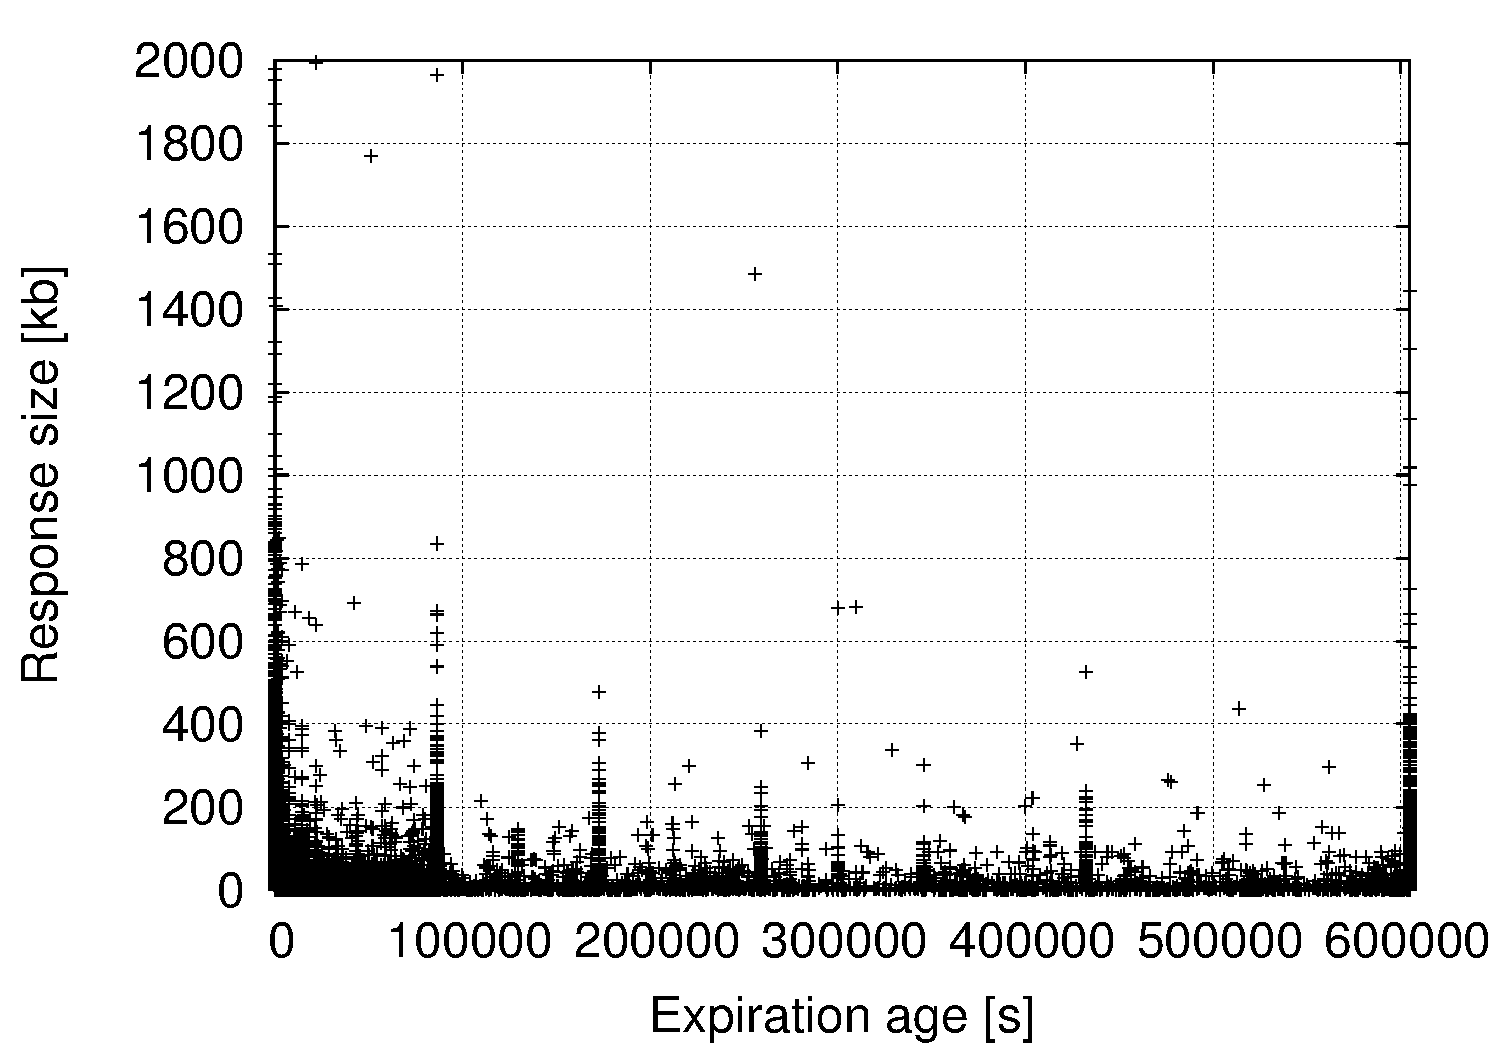
\includegraphics[width=2.75in]{scatterplots/overall_2d_scatterplot_respSizes_expAges-eps-converted-to}}
	\hfil
	%\qquad
	%
	\subfloat[Mobile Web Pages \label{fig:prel}]{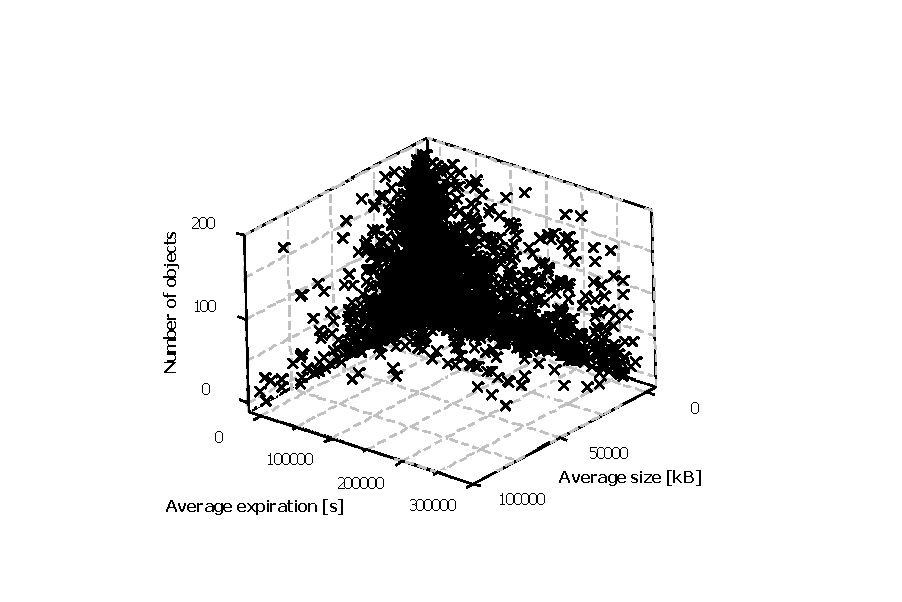
\includegraphics[width=2.75in]{scatterplots/scatter}}
	%
	\caption{Individual sizes and cache expirations for 197634 web objects as well as their averages when considering page--level relationships for 4776 mobile web landing pages.\label{fig:rel}}
\end{figure*}

Initially, we observe that the distribution of object sizes over their lifetime is spread across the entire range of evaluated times. 
We secondly note that at specific expiration times, i.e., none, hour, day, etc., a broader range and aggregation of objects can be observed. 
While we do not observe a close correlation of object sizes and their cache lifetimes, we note that large numbers of even large sized objects have a very short lifetime.

Next, we evaluate the aggregated sizes on a page level in Figure~\ref{fig:prel}, whereby we focus on the range of below 100 objects, expiration below the first several days of a week, and up to 100 kB object sizes.
We observe that the majority of web pages in this group exhibits a low average expiration age as well as a generally small average object size.
We additionally observe that the number of objects on a web page is fluctuating widely for this data set.
Overall, we do not observe a direct relationship between the number of objects, their overall sizes, and their expiration ages once we evaluate them contextually combined on the web page level.
We employ this observation in the following modeling approach.


\section{Object--Level Modeling}
\addcontentsline{toc}{section}{Object--Level Modeling}
\label{s:object}
The initial modeling approach targets the level of individual objects as present in the entire data set, i.e., across all mobile web pages. 
This approach hence would be suitable for high--level modeling of mobile web traffic characteristics.

\subsection{Object Sizes}
\addcontentsline{toc}{subsection}{Object Sizes}
The individual object sizes follow a Weibull minimum distribution, which we employ to randomly draw individual object sizes $x_o$ as defined by 
\begin{equation}\label{eq:weibull}
f\left(x_o\right) = \frac{a}{\lambda} \left(\frac{x_o}{\lambda}\right)^{a-1} \cdot e^{-(x_o/\lambda)^a}, 
\end{equation}
with $x_o>0, \alpha>0$.
We identified the shape parameter as $a \cong  0.573$ and the scale parameter as $\lambda \cong 8887.5$.
We illustrate the results from 500 evaluations in Figure~\ref{fig:osize}, noting that we omit the illustration of the confidence intervals for readability (they are typically within ten percent of the original value).

We observe that both distributions peak at a small response size on drop immediately, with the simulated web page object sizes following the trend of the underlying data set closely.
Due to the nature of the selected Weibull distribution for simulation purposes, the smaller abrupt changes in the distribution of sizes visible for the source data, e.g. between object sizes of 10 kB and 20 kB, are not captured in the modeled distribution.
We reason that the tractability and otherwise close fit, however, outweigh the capturing of these minor irregularities.


\subsection{Object Expiration Ages}
\addcontentsline{toc}{subsection}{Object Expiration Ages}
Next, we evaluate the capturing of the expiration ages, i.e., the maximum cache lifetime, of the individual web objects found in the dataset.
The underlying notion of web server configurations exhibits a non--linear relationship between the individual object expiration times set $t_o$, whereby common time frames, such as mandatory hourly or daily refreshes of individual objects are common. 
In turn, the modeling of this particular behavior follows a piecewise approximation, which distributes the expiration ages based on their original frequency in the underlying data set within the one week time interval we consider here.
Denoting $U(a,b)$ as a continuous uniform distribution between inclusive $a$ and $b$ and $U[a,b]$ its discrete counterpart, we model the mobile web object expiration times by initially drawing $\tau_o \sim U(0,1)$ randomly.
We subsequently determine the expiration age $t_o$ for the object under consideration as in Eq.~\ref{eq:t0}.
\begin{equation*}\label{eq:t0}
t_o =
\begin{cases}
0 ~\mathrm{for}~ 0 \le \tau_o <  0.6108,\\
300 ~\mathrm{for}~ 0.6108 \le  \tau_o < 0.6235,\\
600 ~\mathrm{for}~ 0.6235 \le \tau_o < 0.6353,\\
900 ~\mathrm{for}~ 0.6353 \le \tau_o < 0.6460,\\
3600 ~\mathrm{for}~0.6460 \le \tau_o < 0.6887,\\
7200 ~\mathrm{for}~0.6887 \le \tau_o < 0.6970,\\
14400 ~\mathrm{for}~0.6970 \le \tau_o < 0.7070,\\
21600 ~\mathrm{for}~0.7070 \le \tau_o < 0.7152,\\
43200 ~\mathrm{for}~0.7152 \le \tau_o < 0.7333,\\
86400 ~\mathrm{for}~0.7333 \le \tau_o < 0.8037,\\
172800 ~\mathrm{for}~0.8037 \le \tau_o < 0.8126,\\
604800 ~\mathrm{for}~0.8126 \le \tau_o < 0.8909,\\
U[0, 604800]~\mathrm{otherwise}.
\end{cases}
\end{equation*}

\begin{figure}[b!]
	\centering
	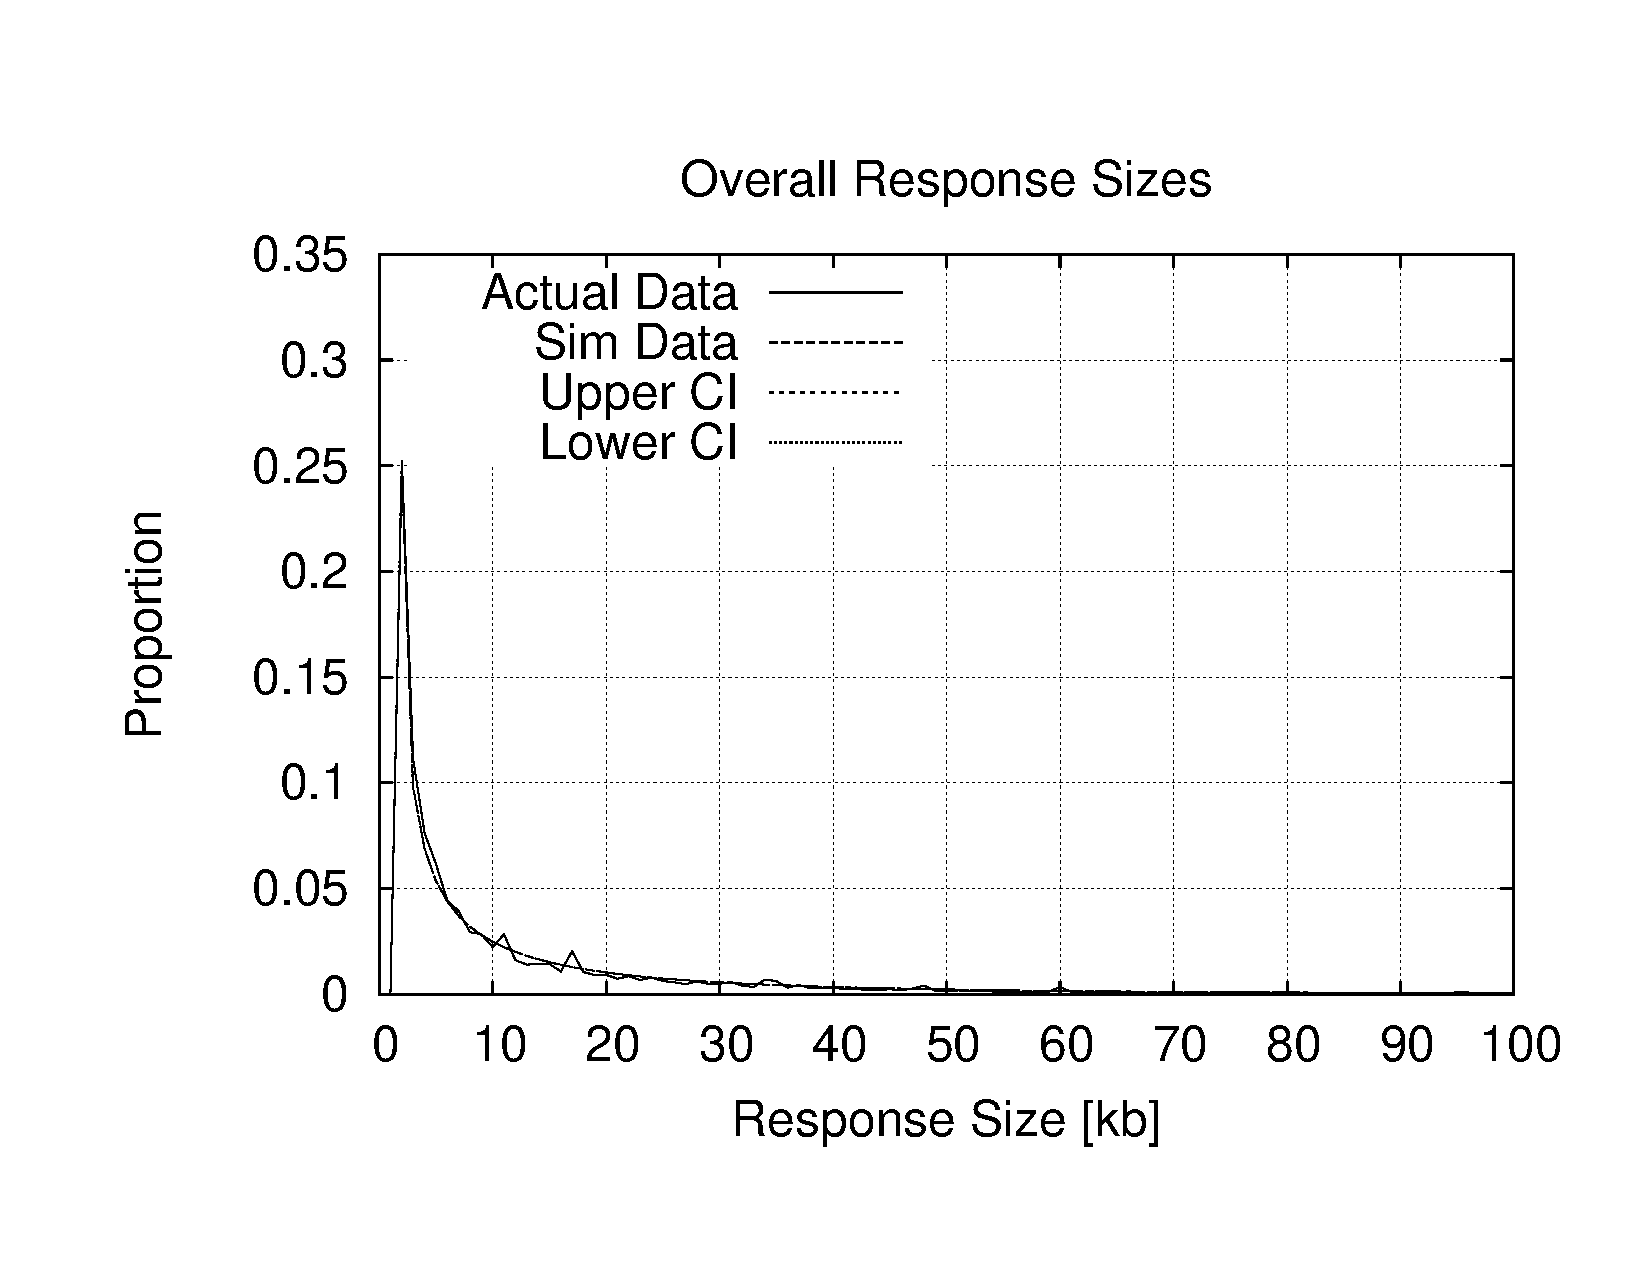
\includegraphics[width=.33\textwidth,angle=270]{respSizes/Overall/overall_respSizes}
	\caption{Real data set and synthetically generated web page object sizes across the entire data set.}
	\label{fig:osize}
\end{figure}

We illustrate the original data set and simulated values in Figure~\ref{fig:oexp}.
\begin{figure}[b]
	\centering
	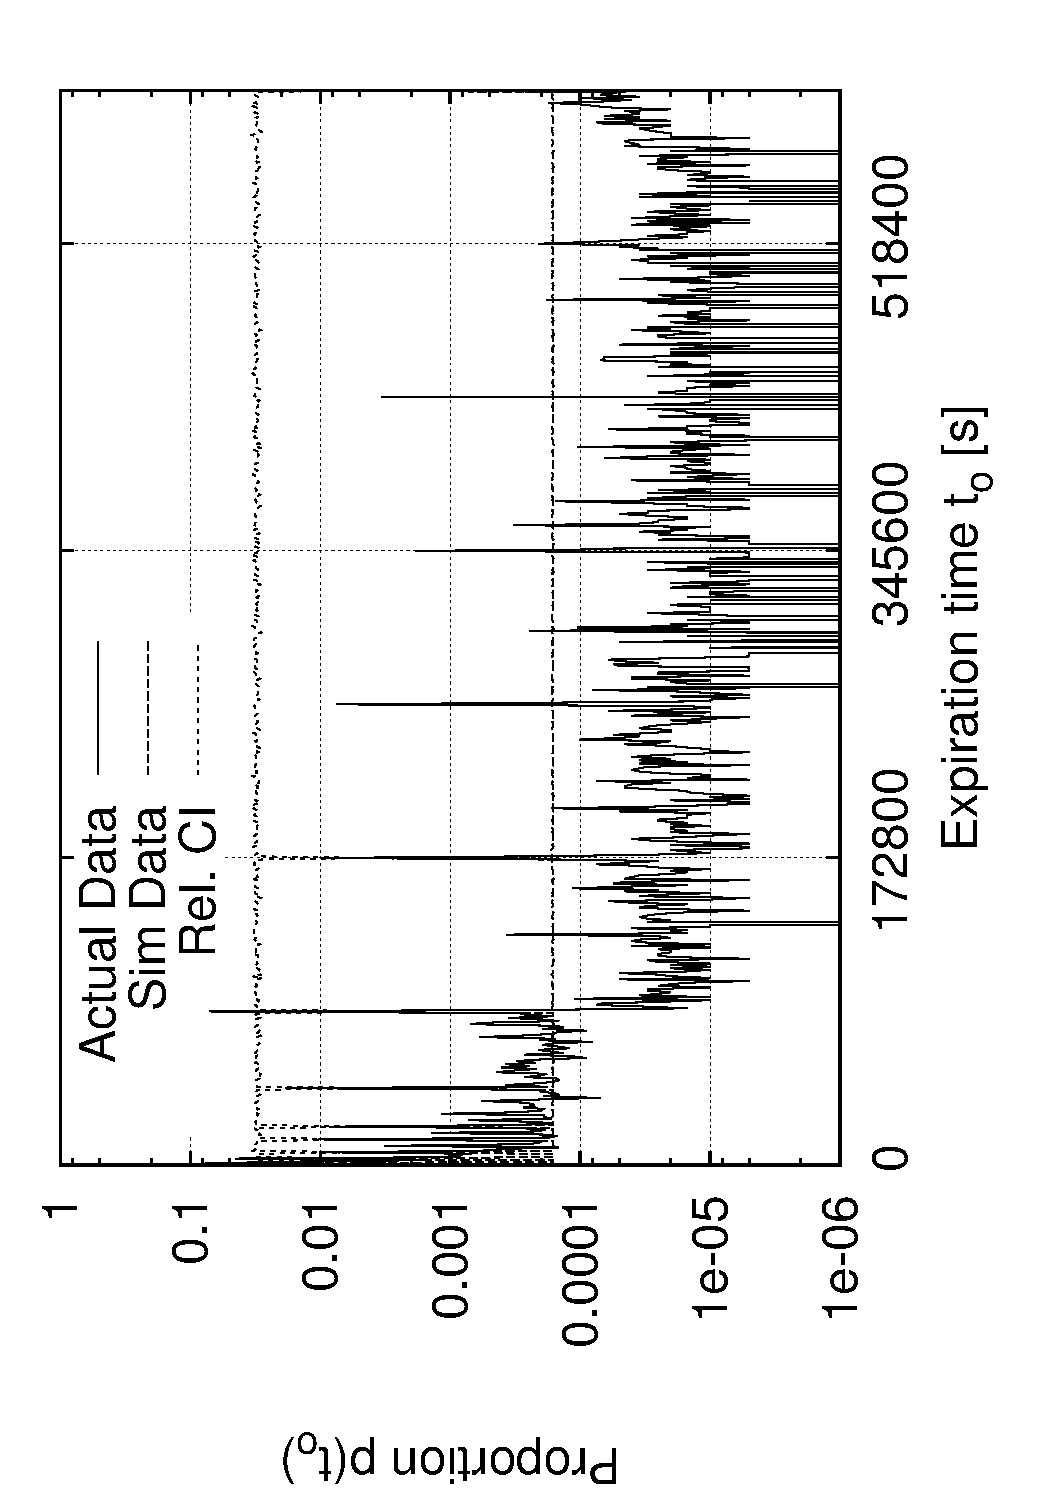
\includegraphics[width=.33\textwidth,angle=270]{expAges/Overall/overall_expAges-eps-converted-to}
	\caption{Real data set and synthetically generated web page object expiration ages across the entire data set.}
	\label{fig:oexp}
\end{figure}
We observe that the original expiration times exhibit several ``spikes'' of higher probability at the common time instances for mandatory cached element refreshes. 
This trend of expirations motivates a piece--wise approximation instead of fully capturing the detailed characteristics for the entire time scale.
Our model approaches the generally compartmentalized structure of expiration times especially for the shorter time scales of common values and coarsely approximates the longer tail end with smaller numbers of objects.


\section{Page--Level Modeling}
\addcontentsline{toc}{section}{Page--Level Modeling}
\label{s:page}
The modeling of the web pages is based on the combination of modeling the number of objects, their sizes, and their expiration times.
In contrast to the individual object level, we now need to consider the mobile web page--level context for the expiration age distributions, especially those objects that cannot be cached.
In the following, we present the individual model approach by the respective component.

\begin{figure}[t!]
	\centering
	\subfloat[Average number of objects per mobile web page	\label{fig:preq}]
	{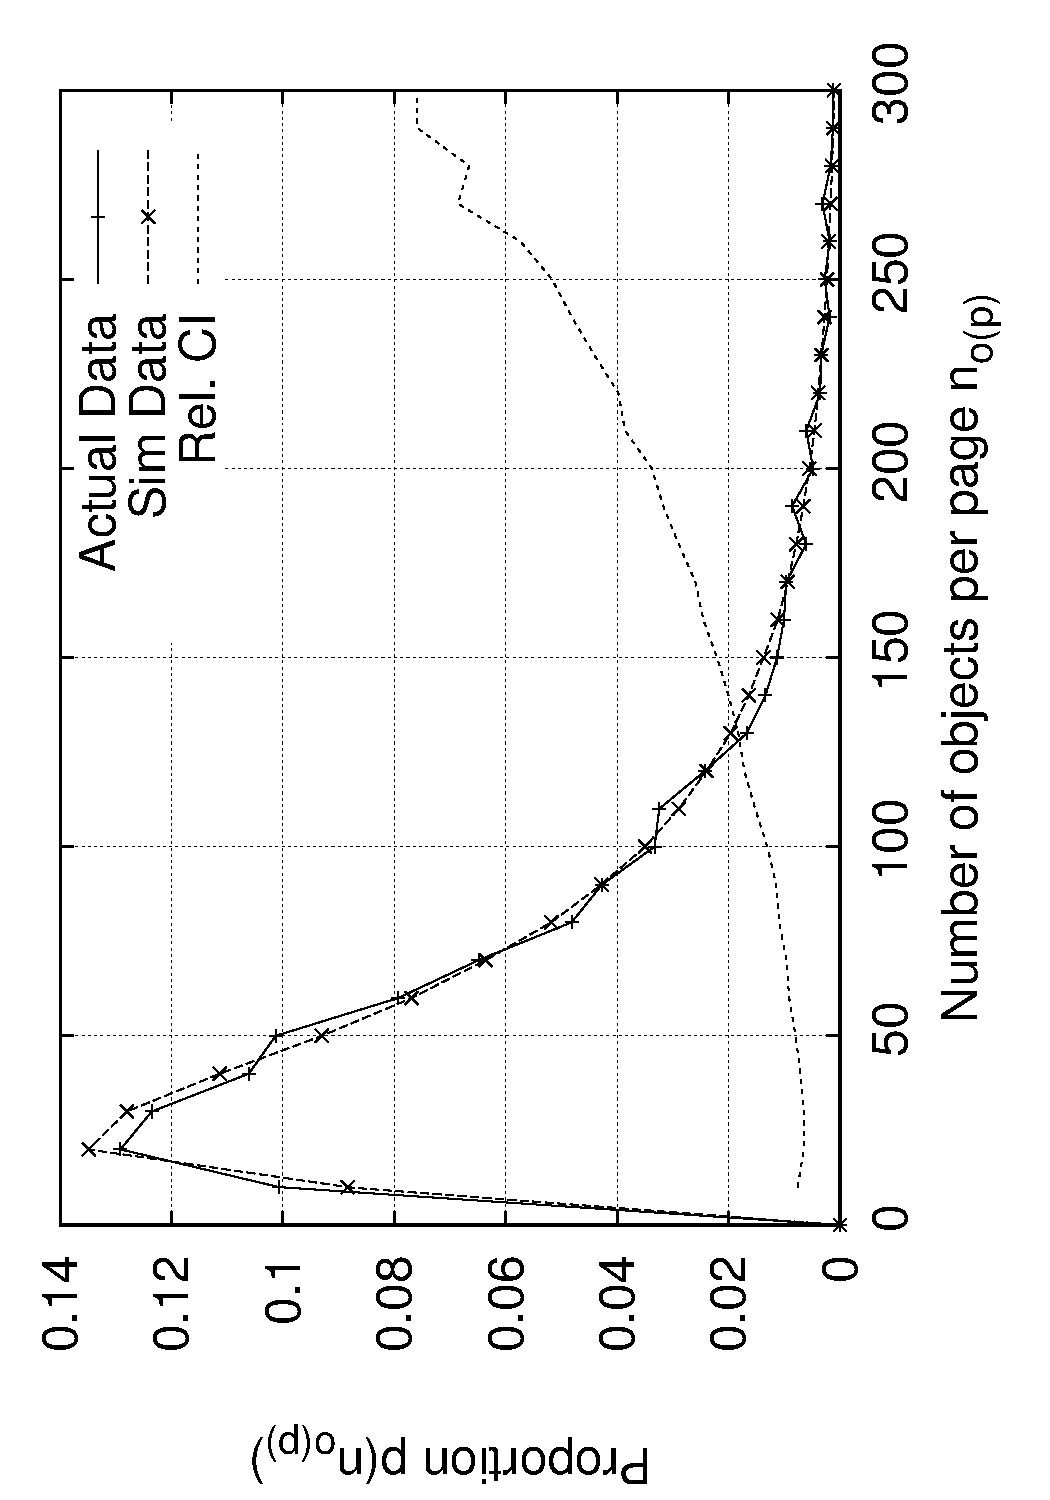
\includegraphics[width=.34\textwidth,angle=270]{numResponses/numResponses-eps-converted-to}}
	\qquad
	\vspace{.1in}
	%
	\subfloat[Mobile web page sizes\label{fig:psize}]
	{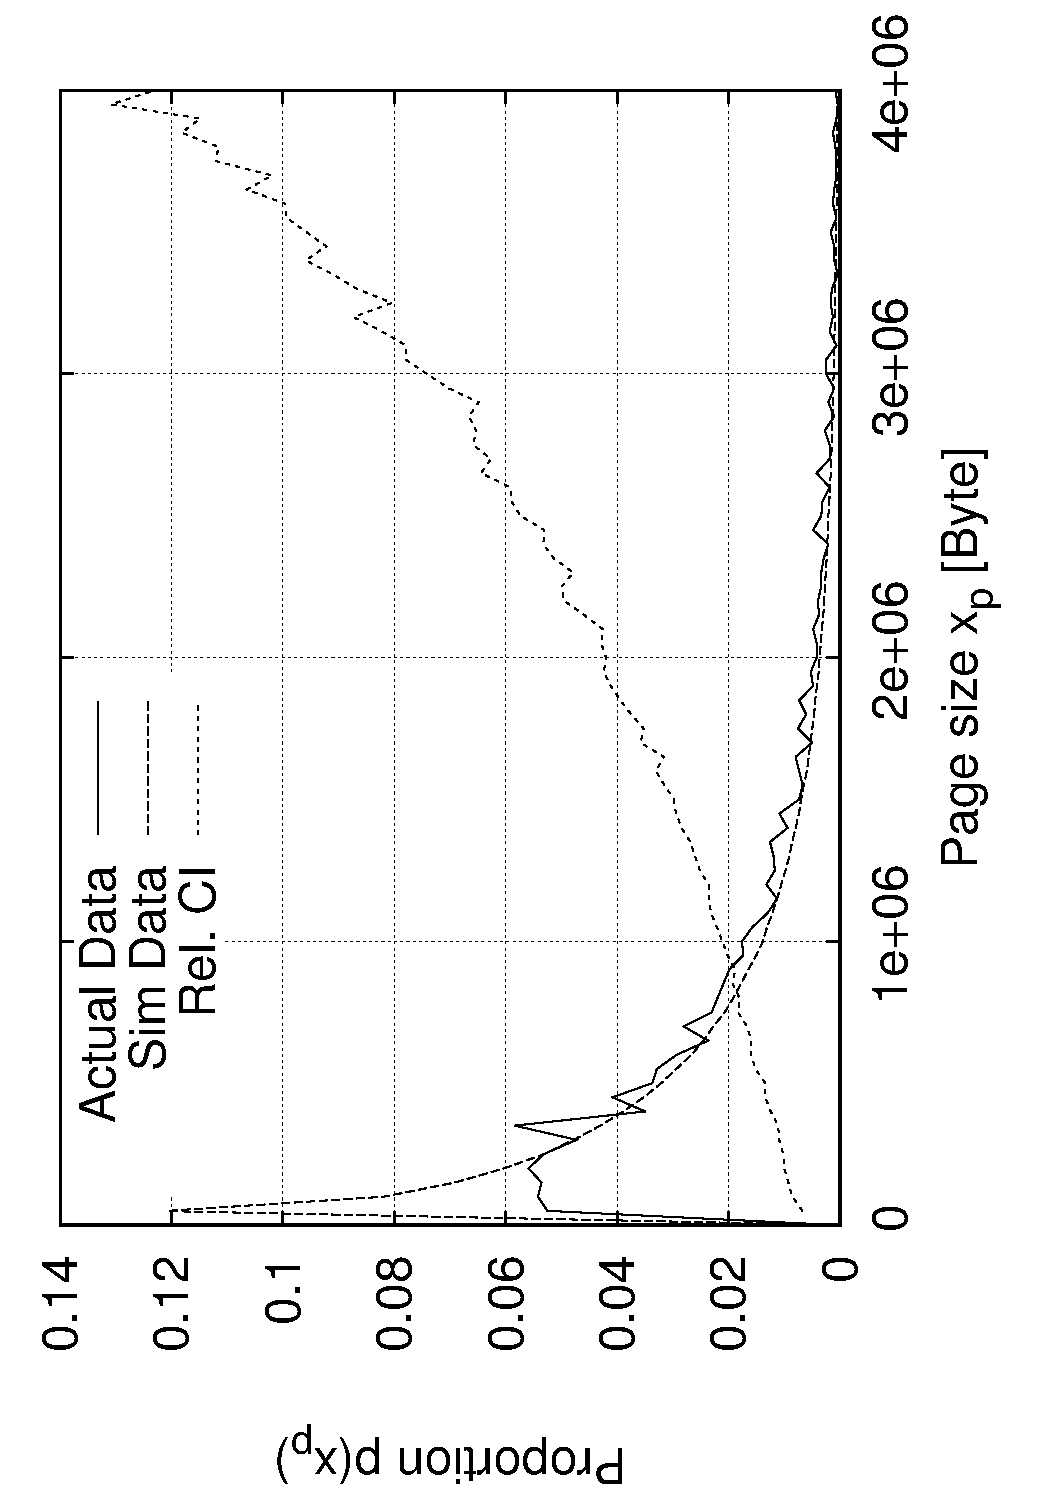
\includegraphics[width=.34\textwidth,angle=270]{respSizes/PageLevelTotal/page_level_sum_respSizes-eps-converted-to}}
	\qquad
	\vspace{.1in}
	%
	\subfloat[Average mobile web page object expiration\label{fig:pexp}]
	{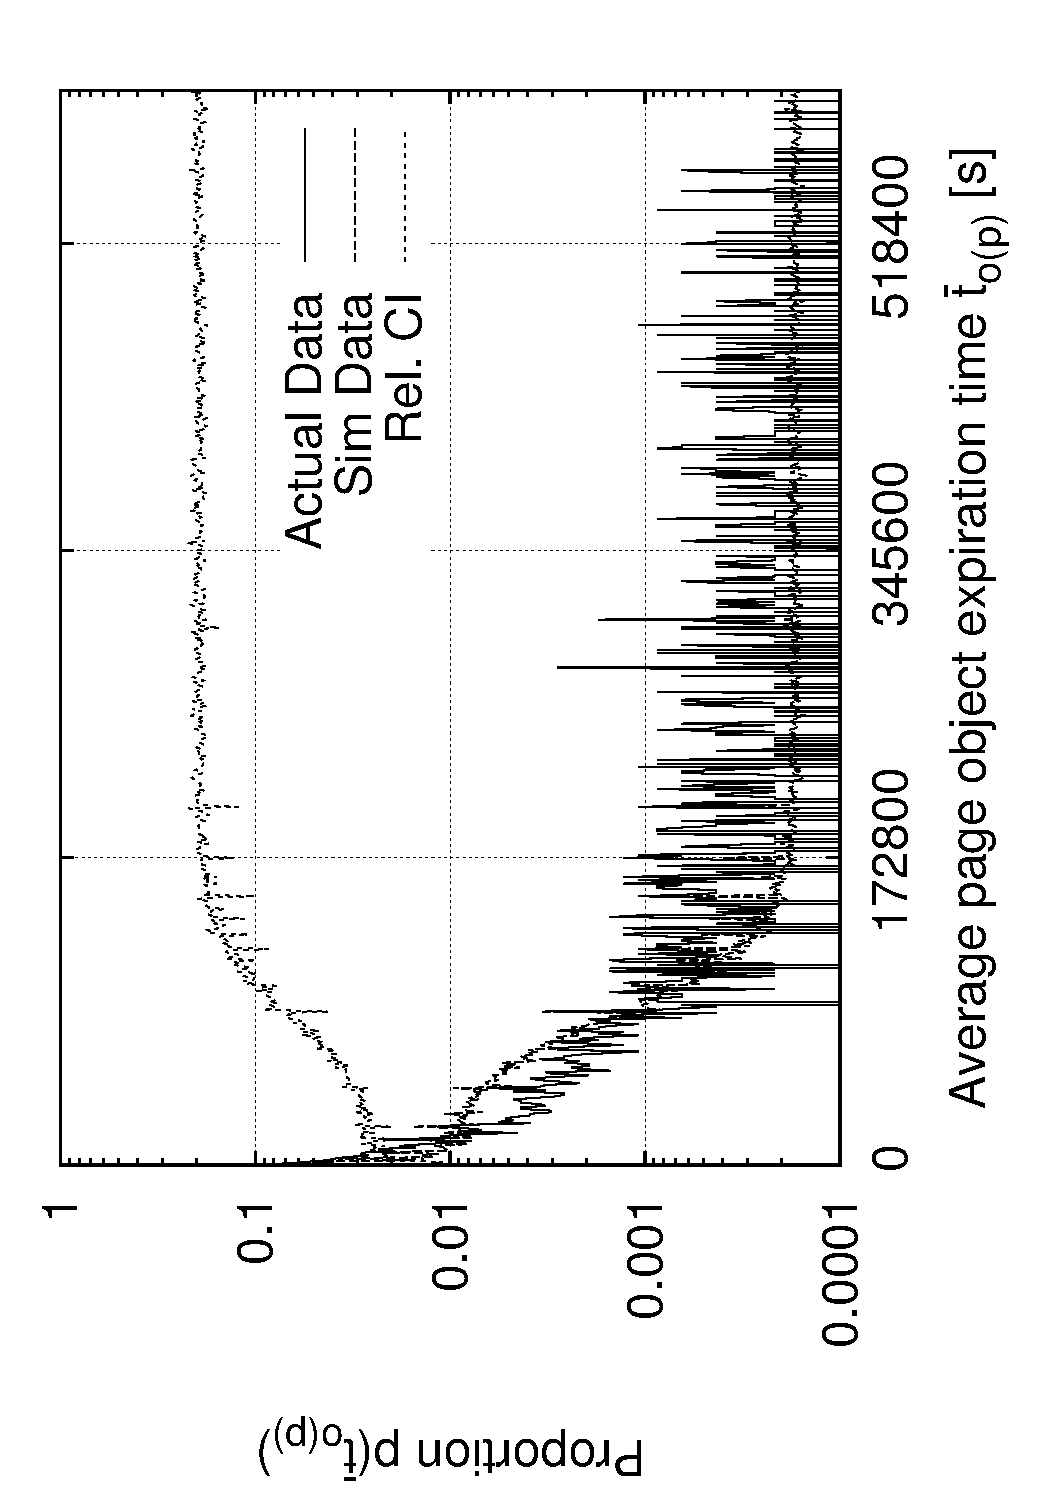
\includegraphics[width=.34\textwidth,angle=270]{expAges/PageLevelAverages/PageLevelexpAgeAverage/page_level_average_expAges-eps-converted-to}}
	\qquad	
	\vspace{.1in}
	%
	\caption{Page--level simulation of mobile web landing pages for the October 15, 2013 data set.\label{fig:pages}}
\end{figure}

\subsection{Number of Objects per Page}
\addcontentsline{toc}{subsection}{Number of Objects per Page}
The evaluation of the aggregated object numbers $n_{o(p)}$ for the individual pages $p$ indicates a distribution that follows a general Gamma distribution as 
\begin{equation}\label{eq:gg}
f\left( n_{o(p)} \right) = \frac{ k \cdot (n_{o(p)})-\gamma)^{\kappa\alpha-1} }{\beta^{\kappa\alpha}\Gamma(\alpha)}e^{-\left(\frac{n_{o(p)}-\gamma}{\beta}\right)^\kappa},
\end{equation}
whereby we determine the two shape parameters as $\alpha=3.1119, \kappa=0.6167$, the scale parameter $\beta=8.2912$, and the location parameter as $\gamma=0.17238$.
​
We illustrate the resulting outcome in Figure~\ref{fig:preq} as a comparison between original and simulated data, as well as the  width of the confidence interval in relation to the simulated data.
We observe that the average number of objects per page in both the original and simulated page data sets exhibit the same sharply rising distribution with a significantly longer tail of pages comprised of more than 25 objects.
We furthermore observe that the relative confidence interval width exhibits an increasing trend as the number of objects increases up to about 8 \%. 
This trend originates in the increasingly smaller probabilities of attaining a high number of web page elements. In turn, small deviations have an increasing impact on this relative performance metric. 



\subsection{Average Mobile Web Page Size}
\addcontentsline{toc}{subsection}{Average Mobile Web Page Size}
With the determined number of objects in a page, the next step considers the determination of the individual web page object sizes.
The individual object size on the page level is determined in a next step by employing a Weibull distribution (as in Equation~\ref{eq:weibull}) with $a=0.27 ,\lambda=700$, and location adjusted by 2.5.
The resulting sum of mobile web landing page objects sizes is illustrated in Figure~\ref{fig:psize}.
We observe that the page size distribution for both original and simulated data  exhibits the same trend of mostly smaller web page sizes paired with a long tail end.
The most notable difference between the two data sets occurs in the range of smaller web page sizes below 500 kB, where the original data has a less pronounced peak than the simulated data.
The relative confidence interval values follow the same trend we previously observed in Figure~\ref{fig:preq} for the number of requests.
Specifically, the relative width of the confidence interval increases with the page sizes and the decline of their respective probability.
We follow the prior reasoning that the significantly reduced probability towards the tail end is responsible for this increasing trend.  


\subsection{Average Mobile Web Page Expirations}
\addcontentsline{toc}{subsubsection}{Average Mobile Web Page Expirations}
As a last step, we determine the expiration ages for the individual web page objects, but now with a contextual consideration for their distribution within the underlying mobile web pages as $t_o^p$.
We separate pages into different categories as ($i$) current, ($ii$) short--lived, ($iii$) medium--lived, and ($iv$) regular.

\subsubsection{Current Pages}
\addcontentsline{toc}{subsubsection}{Current Pages}
Current pages are characterized by all of their objects exhibiting a zero cache lifetime, and thus require extensive downloads. 
They account for approximately 6.3 \% of the pages in the simulated data set.

\subsubsection{Short--lived Pages}
\addcontentsline{toc}{subsubsection}{Short--lived Pages}
This page category exhibits a low expiration age for all its objects and accounts for approximately 24.1 \% of all pages.
The expiration age for all objects is determined following the piece--wise approach in Equation~\ref{eq:t0}, but with modified ranges and probabilities as in Equation~\ref{eq:t1} as 
\begin{equation}\label{eq:t1}
t_{o(p)} =
\begin{cases}
300 ~\mathrm{for}~ 0 \le \tau_o < 0.088, \\
1200 ~\mathrm{for}~ 0.088 \le \tau_o < 0.158, \\
1800 ~\mathrm{for}~0.158\le \tau_o < 0.246,\\
3600 ~\mathrm{for}~0.246 \le \tau_o < 0.351,\\
7200 ~\mathrm{for}~0.351 \le \tau_o < 0.404,\\
14400 ~\mathrm{for}~0.404 \le \tau_o < 0.456,\\
21600 ~\mathrm{for}~0.456 \le \tau_o < 0.474,\\
U[0, 604800]~\mathrm{otherwise}.
\end{cases}
\end{equation}

\subsubsection{Medium-lived Pages}
\addcontentsline{toc}{subsubsection}{Medium-lived Pages}
The long--lived page category exhibits a heavier tail for the expiration ages of its objects.
In turn, we employ a log--logistic distribution to model the expiration ages of all objects as 
\begin{equation}
f(t_{o(p)})=\frac{\beta}{\alpha} \left(\frac{t_{o(p)}-\gamma}{\alpha}\right)^{\beta-1}\left(1+\left(\frac{t_{o(p)}-\gamma}{\alpha}\right)^\beta\right)^{-2},
\end{equation}
whereby we set scale parameter $\alpha \approx 0.889 $, shape parameter $\beta \approx 2600.7$, and location parameter $\gamma=1$. 
When drawing a random expiration age, we limit the upper end of expiration ages to 43200.

\subsubsection{Regular Pages}
\addcontentsline{toc}{subsubsection}{Regular Pages}
Regular pages account for the majority 63.3 \% of the simulated web pages. 
Their simulation is a two--step process, which initially determines the number of non--cacheable objects $c^0_{o(p)} \in [0,1]$ as a sample from a normal distribution with $\lambda \approx 0.629, \sigma \approx 0.301$.
In a second step, the remaining expiration ages are set according to 
\begin{equation*}
t_{o(p)} =
\begin{cases}
	0	~\mathrm{for}~	0.000	\le \tau_o <	0.611,                \\
	43200	~\mathrm{for}~	0.611	\le \tau_o <	0.629,            \\
	U[43201,86400]	~\mathrm{for}~	0.629	\le \tau_o <	0.641,   \\
	86400	~\mathrm{for}~	0.641	\le \tau_o <	0.885,            \\
	U[86401,172800]	~\mathrm{for}~	0.885	\le \tau_o <	0.889,  \\
	172800	~\mathrm{for}~	0.889	\le \tau_o <	0.898,           \\
	U[172801,259200]	~\mathrm{for}~	0.898	\le\tau_o <	0.900, \\
	259200	~\mathrm{for}~	0.900	\le \tau_o <	0.908,          \\
	U[259201,604800]	~\mathrm{for}~	0.908	\le \tau_o <	0.922, \\
	604800	~\mathrm{otherwise}.
\end{cases}
\end{equation*}

Comparing the thus generated expiration times with those found in the original data set in Figure~\ref{fig:pexp}, we observe that the average page object expiration ages follow the same decreasing trend.
We furthermore note that the underlying data set exhibits a significantly higher level of variability in the average page object expiration ages than the simulated data. 
Additionally, we also observe that the simulated data features a slightly increased probability of shorter average expiration ages up to a day.
We note that the relative confidence interval width increases from very narrow to a steady 20 \% of the simulated data 
for the tail end of the average page level expiration ages. 
As visible, here the underlying dataset itself exhibits significant variability, which together with the lower probabilities can be regarded as the main source for the heightened relative confidence interval width.

\section{Evaluation}
\addcontentsline{toc}{section}{Evaluation}
\label{s:eval}
We now employ our model to evaluate its capability to capture web caching characteristics as outlined in, e.g., \cite{JoSe14GreenComm}, through simulations.
We initially assume that all web page objects in the data set have to be cached and evaluate the amount of resulting data that remains in the cache, employing our model in 1000 simulations. 
We compare the results to the original dataset in Figure~\ref{fig:simoct13}.  

(We additionally note that we omit confidence intervals for clarity, as their width is typically within 1 \%).
We observe that the original cached data amount quickly reduces to only about 45 \%, which is attributed to the frequent immediate expiration of objects.
As time progresses, the amounts of data that remain in the cache exhibit a staircase behavior, increasing at common time boundaries, such as an hour or a day.
We note that the simulated cached contents are initially underestimated, by a margin of about 10 \%. 
As time progresses, the model--based estimation follows the original data's trend and slightly underestimates the cached data amounts approximately after 30 minutes.
We observe that the underestimation, however, remains close to the original data, with deviation peaking around 5 \%.

\begin{figure}
	\centering
	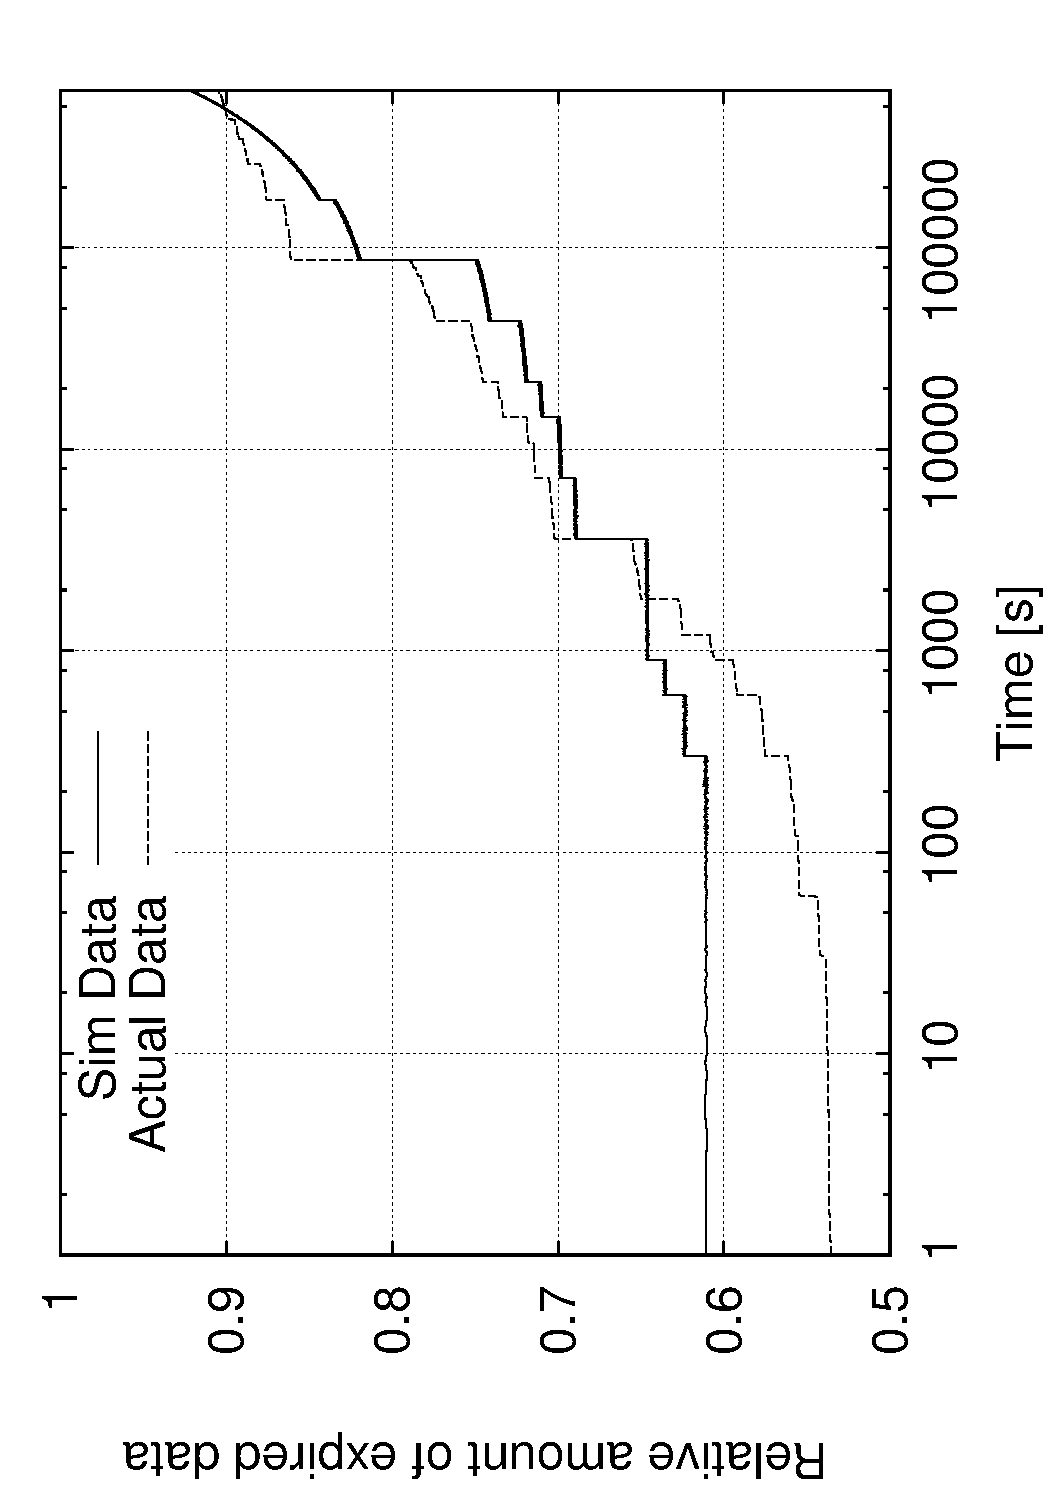
\includegraphics[width=.33\textwidth,angle=270]{modeling_months_cache/oct13/mobile_bytes_graphs-eps-converted-to}
	\caption{Results from evaluations 1000 cache simulations employing the model for Oct. 15, 2013. Our model captures the trends for the overall amounts in the cache over time.\label{fig:simoct13}}
\end{figure}

Overall, we conclude that our model successfully captures the overall trend for the objects of mobile landing web pages, including the approximation of cached amounts data over time. 

\section{Conclusion}
\addcontentsline{toc}{section}{Conclusion}
\label{s:conc}
We described an approximation to model the behavior of popular mobile web landing pages, which are used as upper limit approximation of data that can be expected to require networked delivery to mobile clients.
Our model is based on the assumption that the distribution of object expirations over time does not change significantly as time progresses, but the composition of web pages rather is sensitive to size changes.

We employ this approach to derive a time--independent approach to the application of our model, which is able to predict the cached amounts or downloaded amounts that are required when considering a large number of popular web pages.
As our model slightly under--estimates the amount of data remaining in a potential cache for up to 30 minutes, its resulting output can be readily applied in that time frame, whereas larger time frame model outputs slightly overestimate the cached amount and require discounting.
In future works, we intend to evaluate the model on a finer--grained approach, incorporating the different types of objects constituting the simulated mobile pages.\
\chapter{CONCLUSION}

	
\subsection*{Future Work}
\addcontentsline{toc}{subsection}{Future Work}



\end{Spacing}
\bibliographystyle{unsrt}
\bibliography{main}
\end{document}
